% This is the Reed College LaTeX thesis template. Most of the work
% for the document class was done by Sam Noble (SN), as well as this
% template. Later comments etc. by Ben Salzberg (BTS). Additional
% restructuring and APA support by Jess Youngberg (JY).
% Your comments and suggestions are more than welcome; please email
% them to cus@reed.edu
%
% See http://web.reed.edu/cis/help/latex.html for help. There are a
% great bunch of help pages there, with notes on
% getting started, bibtex, etc. Go there and read it if you're not
% already familiar with LaTeX.
%
% Any line that starts with a percent symbol is a comment.
% They won't show up in the document, and are useful for notes
% to yourself and explaining commands.
% Commenting also removes a line from the document;
% very handy for troubleshooting problems. -BTS

% As far as I know, this follows the requirements laid out in
% the 2002-2003 Senior Handbook. Ask a librarian to check the
% document before binding. -SN

%%
%% Preamble
%%
% \documentclass{<something>} must begin each LaTeX document
\documentclass[12pt,twoside]{reedthesis}
% Packages are extensions to the basic LaTeX functions. Whatever you
% want to typeset, there is probably a package out there for it.
% Chemistry (chemtex), screenplays, you name it.
% Check out CTAN to see: http://www.ctan.org/
%%
\usepackage{graphicx,latexsym}
\usepackage{amsmath}
\usepackage{amssymb,amsthm}
\usepackage{longtable,booktabs,setspace}
\usepackage{chemarr} %% Useful for one reaction arrow, useless if you're not a chem major
\usepackage[hyphens]{url}
% Added by CII
\usepackage{hyperref}
\usepackage{lmodern}
\usepackage{float}
\floatplacement{figure}{H}
% End of CII addition
\usepackage{rotating}

% Next line commented out by CII
%%% \usepackage{natbib}
% Comment out the natbib line above and uncomment the following two lines to use the new
% biblatex-chicago style, for Chicago A. Also make some changes at the end where the
% bibliography is included.
%\usepackage{biblatex-chicago}
%\bibliography{thesis}


% Added by CII (Thanks, Hadley!)
% Use ref for internal links
\renewcommand{\hyperref}[2][???]{\autoref{#1}}
\def\chapterautorefname{Chapter}
\def\sectionautorefname{Section}
\def\subsectionautorefname{Subsection}
% End of CII addition

% Added by CII
\usepackage{caption}
\captionsetup{width=5in}
% End of CII addition

% \usepackage{times} % other fonts are available like times, bookman, charter, palatino

% Syntax highlighting #22

% To pass between YAML and LaTeX the dollar signs are added by CII
\title{From Interpolation to Imputation: Ballot Completion in a Ranked Choice Election}
\author{Jay Lee}
% The month and year that you submit your FINAL draft TO THE LIBRARY (May or December)
\date{May 2019}
\division{Mathematics and Natural Sciences}
\advisor{Heather Kitada Smalley}
\institution{Reed College}
\degree{Bachelor of Arts}
%If you have two advisors for some reason, you can use the following
% Uncommented out by CII
% End of CII addition

%%% Remember to use the correct department!
\department{Mathematics - Statistics}
% if you're writing a thesis in an interdisciplinary major,
% uncomment the line below and change the text as appropriate.
% check the Senior Handbook if unsure.
%\thedivisionof{The Established Interdisciplinary Committee for}
% if you want the approval page to say "Approved for the Committee",
% uncomment the next line
%\approvedforthe{Committee}

% Added by CII
%%% Copied from knitr
%% maxwidth is the original width if it's less than linewidth
%% otherwise use linewidth (to make sure the graphics do not exceed the margin)
\makeatletter
\def\maxwidth{ %
  \ifdim\Gin@nat@width>\linewidth
    \linewidth
  \else
    \Gin@nat@width
  \fi
}
\makeatother

\renewcommand{\contentsname}{Table of Contents}
% End of CII addition

\setlength{\parskip}{0pt}

% Added by CII

\providecommand{\tightlist}{%
  \setlength{\itemsep}{0pt}\setlength{\parskip}{0pt}}

\Acknowledgements{
To Heather, for consistently keeping me on track to actually graduate and being a wonderful thesis advisor;

\par
 \bigskip

\noindent To Andrew, Paul G., Kristin, and Paul M., for giving me a series of good jobs and unofficially advising me over the last few years;

\par
 \bigskip

\noindent To the Reed Collegium Musicum and the Anna Men, for giving me a few hours a week to take my mind off of this and make some music;

\par
 \bigskip

\noindent To Mia, Monika, Jade, and Scottie's Gang, for each giving me a semblance of a social life and getting me off campus;

\par
 \bigskip

\noindent To my family, for not getting \emph{too} mad at me for not calling as much as I should;

\par
 \bigskip

\noindent Thank you.
}

\Acknowledgements{
To Heather, for consistently keeping me on track to actually graduate and being a wonderful thesis advisor;

\par
 \bigskip

\noindent To Andrew, Paul G., Kristin, and Paul M., for giving me a series of good jobs and unofficially advising me over the last few years;

\par
 \bigskip

\noindent To the Reed Collegium Musicum and the Anna Men, for giving me a few hours a week to take my mind off of this and make some music;

\par
 \bigskip

\noindent To Mia, Monika, Jade, and Scottie's Gang, for each giving me a semblance of a social life and getting me off campus;

\par
 \bigskip

\noindent To my family, for not getting \emph{too} mad at me for not calling as much as I should;

\par
 \bigskip

\noindent Thank you.
}

\Dedication{
\noindent ACS: American Community Survey

\par

\noindent GIS: Geographic information system

\par

\noindent IPW: Inverse probability weighting

\par

\noindent MAR: Missing at random

\par

\noindent MCAR: Missing completely at random

\par

\noindent MI: Multiple imputation

\par

\noindent MLE: Maximum likehood estimation

\par

\noindent MNAR / NI: Missing not at random / Non-ignorable

\par

\noindent PAC: Political action committee

\par

\noindent Q-Q: Quantile-quantile

\par

\noindent RCV: Ranked choice voting

\par

\noindent RHD: Random hot deck

\par

\noindent SE: Standard error

\par

\noindent SF: San Francisco

\par

\noindent STV: Single transferable vote

\par

\noindent VAP: Voting-age population

\par

\noindent VEP: Voting-eligible population

\par
}

\Abbrevs{
\noindent ACS: American Community Survey

\par

\noindent GIS: Geographic information system

\par

\noindent IPW: Inverse probability weighting

\par

\noindent MAR: Missing at random

\par

\noindent MCAR: Missing completely at random

\par

\noindent MI: Multiple imputation

\par

\noindent MLE: Maximum likehood estimation

\par

\noindent MNAR / NI: Missing not at random / Non-ignorable

\par

\noindent PAC: Political action committee

\par

\noindent Q-Q: Quantile-quantile

\par

\noindent RCV: Ranked choice voting

\par

\noindent RHD: Random hot deck

\par

\noindent SE: Standard error

\par

\noindent SF: San Francisco

\par

\noindent STV: Single transferable vote

\par

\noindent VAP: Voting-age population

\par

\noindent VEP: Voting-eligible population

\par
}

\Abstract{
One of the arguments against implementing ranked-choice voting (RCV) is that RCV is harder for voters to participate in. Two of the reasons for this are the more complicated ballot design and the extra effort that goes into forming a ordered preference of candidates. To evaluate this claim, we examine rates of ballot errors and undervoting (ranking fewer than the allowed number of candidates) in some American elections conducted with RCV. Results show that the variables which are significant in predicting RCV ballot completion are similar to those which are significant in predicting voting rates in general.

\par

We further investigate the impact of overvotes and undervotes on an RCV election. By simulating vote choices for those not present in the ballot data, we obtain a number of counterfactual datasets where overvoting and undervoting never occur, and re-tabulate election results with this simulated data. Methods used include hot deck imputation and multinomial logistic regression. Results here show little effect, but indicate promise for further research on the topic.
}

	\usepackage{placeins}
% End of CII addition
%%
%% End Preamble
%%
%
\begin{document}

% Everything below added by CII
  \maketitle

\frontmatter % this stuff will be roman-numbered
\pagestyle{empty} % this removes page numbers from the frontmatter
  \begin{acknowledgements}
    To Heather, for consistently keeping me on track to actually graduate and being a wonderful thesis advisor;
    
    \par
     \bigskip
    
    \noindent To Andrew, Paul G., Kristin, and Paul M., for giving me a series of good jobs and unofficially advising me over the last few years;
    
    \par
     \bigskip
    
    \noindent To the Reed Collegium Musicum and the Anna Men, for giving me a few hours a week to take my mind off of this and make some music;
    
    \par
     \bigskip
    
    \noindent To Mia, Monika, Jade, and Scottie's Gang, for each giving me a semblance of a social life and getting me off campus;
    
    \par
     \bigskip
    
    \noindent To my family, for not getting \emph{too} mad at me for not calling as much as I should;
    
    \par
     \bigskip
    
    \noindent Thank you.
  \end{acknowledgements}
  \begin{abbrevs}
    \noindent ACS: American Community Survey
    
    \par
    
    \noindent GIS: Geographic information system
    
    \par
    
    \noindent IPW: Inverse probability weighting
    
    \par
    
    \noindent MAR: Missing at random
    
    \par
    
    \noindent MCAR: Missing completely at random
    
    \par
    
    \noindent MI: Multiple imputation
    
    \par
    
    \noindent MLE: Maximum likehood estimation
    
    \par
    
    \noindent MNAR / NI: Missing not at random / Non-ignorable
    
    \par
    
    \noindent PAC: Political action committee
    
    \par
    
    \noindent Q-Q: Quantile-quantile
    
    \par
    
    \noindent RCV: Ranked choice voting
    
    \par
    
    \noindent RHD: Random hot deck
    
    \par
    
    \noindent SE: Standard error
    
    \par
    
    \noindent SF: San Francisco
    
    \par
    
    \noindent STV: Single transferable vote
    
    \par
    
    \noindent VAP: Voting-age population
    
    \par
    
    \noindent VEP: Voting-eligible population
    
    \par
  \end{abbrevs}
  \hypersetup{linkcolor=black}
  \setcounter{tocdepth}{1}
  \tableofcontents

  \listoftables

  \listoffigures
  \begin{abstract}
    One of the arguments against implementing ranked-choice voting (RCV) is that RCV is harder for voters to participate in. Two of the reasons for this are the more complicated ballot design and the extra effort that goes into forming a ordered preference of candidates. To evaluate this claim, we examine rates of ballot errors and undervoting (ranking fewer than the allowed number of candidates) in some American elections conducted with RCV. Results show that the variables which are significant in predicting RCV ballot completion are similar to those which are significant in predicting voting rates in general.
    
    \par
    
    We further investigate the impact of overvotes and undervotes on an RCV election. By simulating vote choices for those not present in the ballot data, we obtain a number of counterfactual datasets where overvoting and undervoting never occur, and re-tabulate election results with this simulated data. Methods used include hot deck imputation and multinomial logistic regression. Results here show little effect, but indicate promise for further research on the topic.
  \end{abstract}

\mainmatter % here the regular arabic numbering starts
\pagestyle{fancyplain} % turns page numbering back on

\hypertarget{introduction}{%
\chapter*{Introduction}\label{introduction}}
\addcontentsline{toc}{chapter}{Introduction}

This thesis investigates issues in ranked choice voting (RCV), using a 2018 mayoral election in San Francisco as our observation. It is split into two major parts, each attempting to answer a separate research question. The motivation for these research questions comes out of previous work on RCV with Matthew Yancheff and Mia Leung, advised by Professors Andrew Bray (statistics) and Paul Gronke (political science) at Reed College. Multiple times while presenting this research into RCV, we were asked what the effect would be ``if everybody voted''. To these now-anonymous\footnote{Two years ago, I did not think to write down their names for this purpose.} questioners, I am grateful.

This thesis was written using the \href{https://github.com/ismayc/thesisdown}{\texttt{thesisdown}} R Markdown template for Reed College, created by Chester Ismay. All of the data used, R code, and source documents can be found at my GitHub page: \url{https://github.com/jayleetx/thesis}.

\hypertarget{part-1}{%
\section*{Part 1}\label{part-1}}
\addcontentsline{toc}{section}{Part 1}

Chapters 1-3 investigate the demographic trends associated with the phenomena of overvoting and undervoting in RCV.
\protect\hyperlink{demo-litreview}{Chapter 1} reviews the literature around RCV in general, its implementation in San Francisco, and comparisons between RCV and the more common \emph{plurality} voting system.
\protect\hyperlink{demo-methods}{Chapter 2} describes the methods used to conduct this investigation, particularly the data transformations that were required to obtain usable data.
\protect\hyperlink{demo-results}{Chapter 3} details the results of the investigation, validations of the methods used, and some implications for further research.

\hypertarget{part-2}{%
\section*{Part 2}\label{part-2}}
\addcontentsline{toc}{section}{Part 2}

Chapters 4-6 use missing data imputation methods to simulate a situation where there were no ballot errors, particularly undervoting and undervoting.
\protect\hyperlink{missing-litreview}{Chapter 4} covers the theory around missing data and a comparison of multiple possible methods to deal with this phenomenon.
\protect\hyperlink{missing-methods}{Chapter 5} explains which methods will be used in this study, as well as the problems encountered along the way which had to be dealt with.
\protect\hyperlink{missing-results}{Chapter 6} presents the conclusions from the analysis.

\hypertarget{demo-litreview}{%
\chapter{RCV Background}\label{demo-litreview}}

\hypertarget{what-is-ranked-choice-voting}{%
\section{What is ranked choice voting?}\label{what-is-ranked-choice-voting}}

\emph{Ranked choice voting} (RCV), also known as the \emph{alternative vote} or \emph{instant-runoff voting} is an alternative voting method to the \emph{first-past-the-post} or \emph{plurality} election system more familiar to American voters, where the candidate with the most votes wins. Each voter, instead of choosing their highest preference among a set of candidates for an office, ranks some subset of the candidates in order of preference. This system (or a close variant) is used in Australia, Maine, and some American municipalities: San Francisco, CA; Minneapolis, MN; and Cambridge, MA; among others.

The single-winner RCV tabulation algorithm generally proceeds as follows\footnote{Modified from Arrow, Sen, \& Suzumura (2002).}:
\begin{enumerate}
\def\labelenumi{\arabic{enumi}.}
\item
  For each voter, identify their most preferred candidate that has not yet been eliminated. Count up these preferences by candidate.
\item
  If one candidate has a majority (50\% + 1) of the unexhausted votes, they are declared the winner and counting stops.
\item
  The candidate with the lowest number of votes is eliminated.
\item
  The ballots counted for that candidate are each transferred to the voter's next choice if one exists, or if one does not exist the ballot is ``exhausted'' and removed from counting for further rounds.
\item
  Return to 1.
\end{enumerate}
Most jurisdictions that use RCV have slightly different rules for edge cases and ballot errors, but this algorithm is what distinguishes RCV from other ranked voting systems\footnote{E.g. Borda (``Borda Count,'' n.d.), Condorcet (``Condorcet Method,'' 2008), Contingent (``Electoral Systems,'' 2013), etc.}. A close variant of RCV is the single transferrable vote (STV) method\footnote{More accurately, RCV is the single-winner implementation of the STV algorithm.}, which can be used to elect multiple candidates, e.g.~for a school board, instead of just one. In the US, this is used in Cambridge, MA and Minneapolis, MN to elect multi-member offices (Douglas, 2013).

\hypertarget{frequently-used-terms}{%
\section{Frequently Used Terms}\label{frequently-used-terms}}

Below are some definitions for frequently used terms later on. These are not all ubiquitous (for example, ``undervote'' has another meaning in other voting research), but we define them here for clarity later on.
\begin{itemize}
\item
  \emph{Overvote}: when a voter ranks multiple candidates in the same slot. This slot is typically thrown out entirely in counting, because it's often not possible to determine which candidate was preferred.
\item
  \emph{Undervote}: when a voter does not rank candidates in all of the slots available to them. This is different than other definitions of ``undervote'', which refer to a voter participating in one election on a ballot but not another one. This is not a problem in counting, and is explicitly allowed in the laws of most jurisdictions. A plurality election analog would be voting in high-profile races (e.g.~presidential), but not down-ticket decisions (e.g.~local water board).
\item
  \emph{Skipped vote}: when a voter ranks no candidate at slot \(x\), but ranks a candidate at slot \(y > x\). This is typically not a problem in counting, but different jurisdictions have different rules about whether a voter's ballot is exhausted at this point or continues on to their next ranked choice. Plurality voting has no analog to this, because each race only has one ``ranking'' (first!).
\item
  \emph{Duplicated vote}: when a voter ranks the same candidate for distinct slots \(x\) and \(y\). This is typically not a problem for counting, and the first ranking for the candidate is used. Similar to a skipped vote, plurality voting has no analog to this. When we fit models to discuss undervoting, this category will be included as well under the heading of ``undervoting'' because it is also a form of not ranking as many unique candidates as offered.
\item
  \emph{Ballot exhaustion}: as ballot counting progresses, some ballots will become ``exhausted'' when all the candidates selected are eliminated. Suppose the final count in an election is between candidates B and D, and a voter ranked candidates C-A-E. Their ballot would not be counted in this final round, as they expressed no preference for either candidate B or D. An analogous situation in a plurality election might be voting in the general election but not a runoff, that is only having a say in part of the election.
\end{itemize}
Overvotes, skipped votes, and duplicated votes are really only interpretable as ``ballot mistakes'': for example, even if a voter truly prefers two candidates equally, the ballot instructions (should) make it clear that ranking them at the same slot is not allowed.

\hypertarget{claims-about-rcv}{%
\section{Claims about RCV}\label{claims-about-rcv}}

There are plenty of arguments both for and against implementing RCV in place of plurality in different jurisdictions (see the literature review), but here we'll focus on evaluating one major argument against it - RCV is harder for voters to participate in than a plurality system. There are two major reasons cited for this:
\begin{itemize}
\item
  The physical design of an RCV ballot is usually more complicated than a plurality ballot, because there has to be a system to encode a more full preference among the candidates than just selecting one candidate
\item
  The process of forming a multi-candidate preference inherently takes more mental energy than just choosing a favorite candidate
\end{itemize}
The first facet of this argument should be reflected in ballot errors made by voters. Compared to plurality voting, we expect more errors in an RCV ballot just because the ballot is more complicated. There are also more potentials for error in the RCV system generally. The only ``errors'' in a plurality ballot are incompletely marking a candidate (think incorrect Scantron bubbling, or hanging chads) or overvoting, both of which are potential pitfalls for a ranked choice ballot as well. On top of these, there are the potential errors of duplicated and skipped votes unique to ranked ballots\footnote{These types of errors are not uniform, and some jurisdictions are more forgiving than others about rules for counting these errors. While it may be apparent that a voter who listed the same candidate 3 times (A-A-A) prefers that candidate, a candidate ranking of A-B-A is harder to extract a clear preference from. Skipped votes are where we see the most variance in jurisdiction counting rules: if a voter marks the ballot A-\_-B, skipping the second slot, some jurisdictions will ignore the skip and treat B as the voter's second choice, while others will stop counting after A is eliminated (ignoring their vote for B), and others yet will throw out the ballot entirely.}.

The second facet should be reflected in incomplete ballots filled out by voters. Given that they understand how to encode their preferences on the ballot, there is still the non-trivial task of forming such a preference. Structurally, some of the factors that should affect this incompleteness are:
\begin{itemize}
\item
  The number of candidates running for a position
\item
  The number of candidates voters can rank
\item
  The number of seats elected in a given race
\end{itemize}
This first variable is at the election level (different for every election), the second is at the jurisdiction level, and the third is a mix of both. For a clear example of these differences, consider a \href{https://sfelections.org/results/20161108/data/20161206/d3/20161206_d3.pdf}{2016 San Francisco Board of Supervisors race (District 3)} versus a \href{https://www.cambridgema.gov/election2017/Council\%20Order\%20Round.htm}{2017 Cambridge City Council race}:
\begin{longtable}[]{@{}lll@{}}
\caption{Comparison of RCV rules by jurisdiction}\tabularnewline
\toprule
Factor & San Francisco 2016 & Cambridge 2017\tabularnewline
\midrule
\endfirsthead
\toprule
Factor & San Francisco 2016 & Cambridge 2017\tabularnewline
\midrule
\endhead
Candidates running & 2 & 27\tabularnewline
Candidates rankable & 2 (Generally, up to 3\footnote{This is changing in 2019 to be up to 10.}) & 27 (Generally, all)\tabularnewline
Seats elected & 1 & 9\tabularnewline
\bottomrule
\end{longtable}
\hypertarget{history-of-rcv-in-the-us}{%
\section{History of RCV in the US}\label{history-of-rcv-in-the-us}}

In the United States, there have been two major periods of RCV implementation in various jurisdictions. Between 1915 and 1950, 24 American cities chose to institute RCV as a form of local election. By 1965, however, all of these except for Cambridge, MA had eliminated the policy change. Then, in the 2000s, there was a resurgence of uptake in a different set of American cities\footnote{Mostly in the American West: there are 9 cities west of the Mississippi River \href{https://www.fairvote.org/where_is_ranked_choice_voting_used}{currently using RCV} (``Where is Ranked Choice Voting Used?'' n.d.) and only 4 east of it.}, including Minneapolis and a handful in the San Francisco Bay Area. While Cambridge has consistently used the multi-winner (STV) method to elect City Council and School Board seats, the modern resurgence of RCV almost universally deals with single-winner elections. Research argues that RCV appears in jurisdictions where there is strong multi-party support for the reform - the RCV method itself gives individual parties less power in the election process, so powerful single parties usually don't have reason to support it (Santucci, 2017).

\hypertarget{why-or-why-not-implement-rcv}{%
\section{Why, or why not, implement RCV?}\label{why-or-why-not-implement-rcv}}

\hypertarget{pros}{%
\subsection{Pros}\label{pros}}

\hypertarget{no-secondary-elections}{%
\subsubsection{No secondary elections}\label{no-secondary-elections}}

There are two major types of ``secondary elections'' used in American voting: primary elections and runoff elections. Primaries are used by political parties to select their nominee for a general election, so the voters of any one party aren't split between different candidates. Runoffs are most often used when no candidate in the general election surpasses 50\% of the vote total. Typically the top two candidates from the general election\footnote{Or primary election - seven Southern states require primary winners to obtain 50\% of the vote to get on the general election ballot, and some other states have a requirement of 40\% (Wilson, 2014).} advance to a later runoff. These secondary elections face two main challenges:
\begin{itemize}
\item
  Low turnout. Secondary elections as a whole face low turnout (Ranney, 1972; Wright, 1989). Research shows that people don't actually like voting that much - the more frequently elections are held, the lower turnout will be for all of them generally. Secondary elections increase the number of elections in a period, so this is one possible reason why they generally have low turnout. Further research indicates that holding elections concurrently with a presidential election ``increase{[}s{]} the likelihood that citizens will vote'' (Boyd, 1986). This is seen in off-year Congressional elections, where turnout drops from presidential years. Typically general elections are held concurrently with presidential elections, so secondary elections cannot be held at the same time as a presidential election and they should thus suffer in turnout. This low turnout has consequences for representation in the system. The same research (Ranney, 1972) finds that while primary voters are not ideologically unrepresentative of general election voters, they are both demographically unrepresentative and unrepresentative on some major issues. Traditional knowledge holds that primary voters are more committed partisans than general election voters, leading the eventual candidates in a general election to be polarized away from the ``center'' of political ideas (Hill, 2007).
\item
  High costs. The higher costs associated with secondary elections are a little more intuitive than turnout issues - it takes money to hold elections. Pollworkers have to be paid, facilities have to be reserved, and candidates have to do more campaigning. A 2011 City Council runoff in Plano, TX cost the city an extra \$73,000 (Rush, 2015). A 2012 Alabama runoff for multiple seats cost the state about \$3 million (The Associated Press, 2014).
\end{itemize}
Since RCV eliminates the need for primary and runoff elections while still ensuring majority rule (which is the main reason for these elections), it should avoid the problems of lower turnout and higher costs associated with secondary elections\footnote{Or, at least some of it.}. Summed up, RCV decreases costs and ``boosts turnout via elimination of low-turnout elections'' (Morales, 2018).

\hypertarget{ensures-majority-rule}{%
\subsubsection{Ensures majority rule}\label{ensures-majority-rule}}

In jurisdictions without rules for 50\% minimums, a common phenomenon is a candidate winning an election with less than 50\% of the vote (a plurality, rather than a majority). The major conceptual issue with this is that more people preferred a candidate other than the one who was elected\footnote{The `ideal' for electoral systems is the Condorcet condition: the candidate elected should beat all other candidates in one-on-one contests.}. RCV requires that a winning candidate receive at least 50\% of the votes remaining\footnote{See below for issues with this ``remaining'' concept.}, ensuring that a majority of voters prefer the elected candidate to other candidates.

This is particularly important in jurisdictions with strong third-party support and more than two viable candidates, like Maine. Former Governor Paul LePage, a Republican, won his first election in 2010 with 38.1\% of the vote, compared to Independent Eliot Cutler's 36.7\%\footnote{A margin of about 7,500 votes. Democrat Libby Mitchell received 19\%.}.

\hypertarget{reduces-strategic-voting---spoiler-candidates-and-third-parties}{%
\subsubsection{Reduces strategic voting - spoiler candidates and third parties}\label{reduces-strategic-voting---spoiler-candidates-and-third-parties}}

Strategic voting\footnote{Also known as ``tactical'' or ``insincere'' voting.} is a scenario where a voter does not reflect their true preferences on their cast ballot in order to affect the outcome of the election. For example, a third party supporter may cast their vote for one of the two major party candidates because otherwise they feel like it won't count.

The ``spoiler effect'' is when a third party candidate draws votes away from the ideologically closest major party candidate, thus contributing to the election of the other major party candidate. The most recent large-scale accusation of this was in the 2000 election. Green Party candidate Ralph Nader drew about 3\% of the national vote, more than the margin of victory for George W. Bush over Al Gore\footnote{Admittedly, the margins are less clear-cut than this at the state level, where the margins actually matter for the Electoral College.}. In the especially consequential state of Florida, Nader took 1.6\% of the vote: almost 200 times greater than the margin between the two major party candidates of less than .01 percentage points\footnote{Not to point fingers at Nader alone in this case - while he was the most popular third party candidate by far, all 8 official third-party candidates received more votes than the major-candidate margin of only 537 votes.} (``2000 Presidential General Election Results,'' 2001). Many believed that Nader, generally seen as more liberal than the Democrat Gore, drew votes from the Democratic base that would have helped Gore win the election otherwise. While research into third-party voters casts some doubt on this theory's applicability in 2000\footnote{In short - while Nader's Florida voters potentially would have broken enough for Gore to put him over the top, this was more a factor of the unusually close margin between the two major candidates than anything that Nader aided in particular.}, public opinion still rests on the idea that Nader cost Gore the presidency\footnote{One of the sections of Nader's Wikipedia page is entitled ``Spoiler controversy'' in regards to this election.} (Herron \& Lewis, 2007). In fact, a pro-Republican PAC aired campaign ads promoting Nader in Democratic states in an attempt to pull votes from Gore (Meckler, 2000).

One of the reasons for major party voters to support RCV is that it avoids this spoiler issue. Under a plurality system, voters are discouraged from voting for third-party candidates because it could help elect their least-preferred of the two major candidates - ``the greater of two evils'', so to speak. Under RCV, however, since voters can be heard throughout multiple rounds across separate candidates, third-party voters can vote for their most preferred candidate, then still have their vote count for a better major-party candidate if their first option is eliminated.

Conversely, one of the reasons for third-party voters to support RCV is that it helps third party candidates get elected. Voters can ignore this aforementioned facet of strategic voting\footnote{Or any strategic voting - while not impossible, it's infeasible to vote strategically under RCV (Bartholdi \& Orlin, 1991).} and select their truly preferred candidate. Third-party supporters who were worried about the spoiler effect, then, can vote for their true preference of a third party and not inadvertently help a less-preferred major candidate get elected. As people abandon this strategy, third parties will receive more votes from people no longer worried about the spoiler effect, and this could get third party candidates elected.

\hypertarget{disincentivizes-negative-campaigning}{%
\subsubsection{Disincentivizes negative campaigning}\label{disincentivizes-negative-campaigning}}

Ranked choice voting should incentivize candidates to avoid negative campaigning. In a plurality election (since candidates don't care about voters who are committed to their competitors) a well-thought-out negative campaign will only ostracize voters who were never going to support another candidate in the first place, and perhaps bring more swing voters to their side. Under RCV, however, alienating another candidate's voters could backfire in the event that candidate is eliminated and these voters decide to support your opponent in the next round, causing your defeat. Research supports this - a 2016 study showed that voters in cities using RCV are more satisfied with campaigns than in cities who use plurality methods, and consider the campaign to have a less negative tone overall (Donovan, Tolbert, \& Gracey, 2016). In San Francisco's first RCV election, there were joint fundraisers between candidates, and one district even saw regular ``Candidates Collaborative'' public meetings between many candidates to discuss issues affecting the district, where ``the setting {[}was{]} decidedly congenial'' (Murphy, 2004).

An interesting case study of this phenomena is in the 2018 San Francisco mayoral election (Kukura, 2018). There were three frontrunners heading into election day, all incumbent members of the city's Board of Supervisors: London Breed, Jane Kim, and Mark Leno. As polls showed Breed ahead about a month before the election, Kim and Leno held a joint press conference to endorse the other as voters' second choices. By drawing second-choice votes from the other candidate, the remaining candidate hoped to overcome the gap between them and Breed. In the actual election, the standing when it came time to proceed to the final round of counting was 102,767 for Breed, 68,707 for Leno, and 66,043 for Kim. While a significant proportion of Kim's voters transferred to Leno after her elimination, in the final round Breed surpassed Leno by about 2,000 votes\footnote{Data from (``Ranked Choice Voting Results Table,'' 2018); Figure \ref{fig:sankey} and analysis with Lee \& Yancheff (2019).}.
\begin{figure}
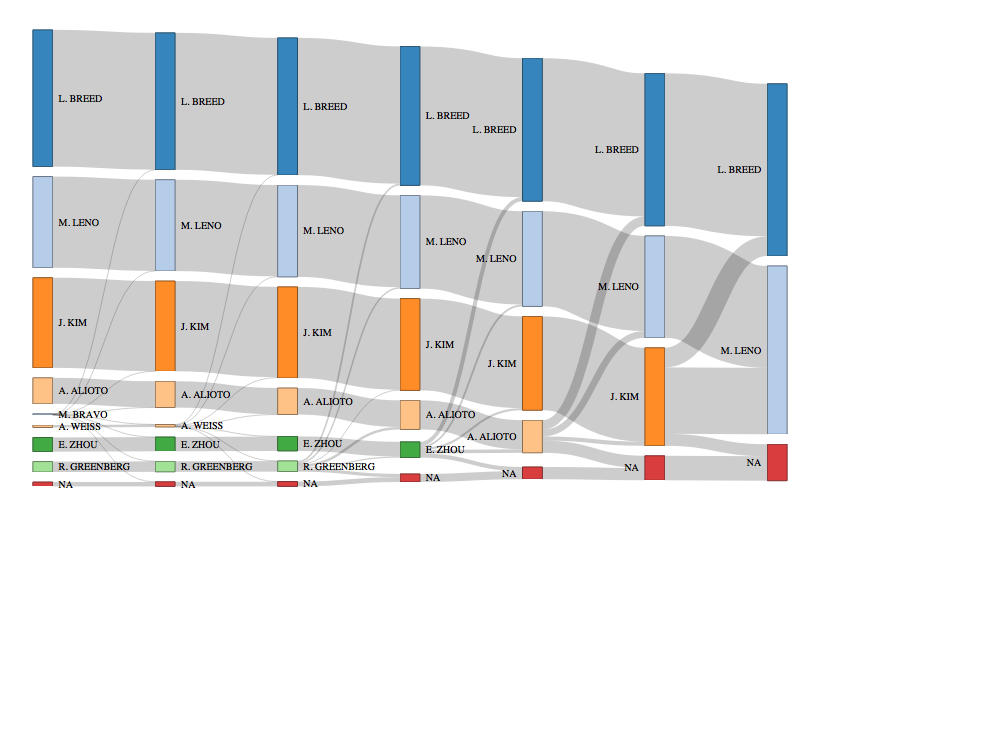
\includegraphics[width=6in]{/Users/jaylee/Desktop/thesis/img/sankey_official_sfmayor18} \caption{Cross-endorsement in SF mayoral race}\label{fig:sankey}
\end{figure}
Though it's outside the scope of this research to tell if this cross-endorsement was effective\footnote{Other confounding factors counld exist: maybe Kim and Leno had similar enough positions that this scenario would have happened without the endorsement, maybe this number is only significant because in the final rounds there were only 2 candidates for second choice votes to flow to, etc.}, there is some evidence in favor of this theory. Leno received almost 70\% of the votes previously counted for Kim compared to Breed's 20\%, bringing Breed's final margin of victory down to only 1 percentage point. In previous rounds of the election, no single candidate ever received more than 35\% of the transferred votes from an eliminated candidate\footnote{Except for round 2, where all 3 votes for the same write-in candidate transferred to Breed.}, so this is at least an unusual observation.

\hypertarget{minority-representation}{%
\subsubsection{Minority representation}\label{minority-representation}}

While much of the American literature on minority representation under voting systems has focused on gerrymandering and single- versus multi-member districts, there is some study of representation under RCV independent of the number of seats up for election. John, Smith, \& Zack (2018) find an increase under RCV in the number of racial and ethnic minority candidates who run in the Bay Area, and an increase in the chance that women and minority women win their election. Their theory for this result is that RCV lowers the barrier to entry in an election, making it more feasible for minority candidates to campaign, and that women (particularly women of color) are better suited in general to the less negative campaigning and coalition-building that RCV promotes in candidates. Another study reports that because minority voter turnout in secondary elections is significantly worse than white turnout (moreso than in a general election), the elimination of these secondary elections should increase the relative say of minority voters in elections overall (Callaghan, 2017).

\hypertarget{turnout-improvements}{%
\subsubsection{Turnout improvements}\label{turnout-improvements}}

Voting system reform advocates claim that these improvements to the voting process will boost turnout by generally increasing public trust in the effectiveness of elections. While there are many different strategies employed by campaigns and advocacy groups to boost turnout, these methods don't have as much effect as changing methods to ranked voting. Phone and direct mail get-out-the-vote campaigns ``typically {[}yield{]} less than 1 percentage point boosts in voter turnout'', and while in-person efforts are better they are less efficient at contacting voters (Morales, 2018).

Another argument is a little less intuitive - ``{[}IRV{]} boosts turnout via elimination of low-turnout elections''. While we typically think about turnout in terms of the number of people voting across similar elections (e.g.~change in turnout from 2010 to 2014 in Congressional races), RCV can improve turnout by increasing the number of people who get to participate in an election overall compared to the number of people who participate in typically low-turnout primary and general elections (Morales, 2018).

\hypertarget{cons}{%
\subsection{Cons}\label{cons}}

\hypertarget{what-is-a-majority-anyway}{%
\subsubsection{What is a majority, anyway?}\label{what-is-a-majority-anyway}}

Under RCV, the problem of ballot elimination can result in ``majorities'' that actually aren't as such. Since it's not always possible to voters to rank every candidate\footnote{This may be disallowed, as SF only allows you 3 rankings (due to technical limitations), or it may just be infeasible - Cambridge often has 20+ candidates on the ballot.}, there will almost certainly be some number of voters who did not list a ranking for any of the candidates still remaining in the final round of the election. Thus the majority that the winner has collected is only a majority of the unexhausted ballots, which may make it less than 50\% of the total counted ballots (Petrangelo, 2013). This does introduce a less expansive form of the spoiler problem - while voters aren't ``punished'' for putting a less electable candidate for their first choice, they are punished for filling all three available slots with minor candidates. In a 2015 study of four RCV elections, Burnett and Kogan found that all four had enough eliminated ballots to only give the winner an overall plurality, not the majority sought after. This is a problem that requires a substantial fix, as ``even individuals who mark three distinct choices often face the prospect of exhaustion, so education alone will not fix the problem'' (Burnett \& Kogan, 2015).

A research question that might address this issue of majorities is whether the pluralities generated by RCV are generally ``bigger'' (closer to the ideal of a true majority) in some way than under plurality, and how this is affected by technical rules like the number of candidates that voters are allowed to rank. Some research\footnote{From the pro-RCV advocacy group FairVote, admittedly.} shows that RCV does perform better than a two-round runoff in this case - as a percentage of the voters in the first round, RCV consistently has more voters counted in the final round compared to top-two runoffs (Richie \& Brown, 2017).

\hypertarget{legal-challenges}{%
\subsubsection{Legal challenges}\label{legal-challenges}}

In addition to the political hurdle of passing RCV legislation\footnote{Neither major party is particularly interested in pushing the issue, and Republicans in particular are often opposed to it (Woodard, 2018).}, there are legal challenges as well. In the aftermath of Maine's recent ballot initiative instituting RCV, legal questions were brought to the state Supreme Court by the State Senate, due to conflict between the initiated bill's language about a ``majority'' versus the state constitution's language requiring a ``plurality''. There was a ruling from the court that resulted in an amended law instituting RCV for only primary elections, but a ``People's Veto'' later occured through initiative that removed the law, followed by a later suit by the state Republican Party to block RCV. Maine has so far used RCV in 2018 for both the primary and general elections to elect certain offices (``Ranked Choice Voting in Maine,'' 2019).

This anecdote examplifies the issue - while public support may be behind RCV in jurisdictions that enact it, legal challenges abound. A (failed) legal challenge was brought against RCV in San Francisco by a defeated candidate in 2011 (Hawkins, 2011). Another challenge (also failed) was brought by Bruce Poliquin against Maine after his loss to Jared Golden in their 2018 Senate race (Mistler, 2018). In Pierce County, WA (home of Tacoma), RCV was repealed by voters after the US Supreme Court court sided with a challenge to reinstate Washington's top two primary-runoff system. With the re-implementation of the top two primary, there was no need to have an RCV election (between two candidates) and the measure was repealed (Eberhard, 2017).

\hypertarget{more-complicated-tabulation}{%
\subsubsection{More complicated tabulation}\label{more-complicated-tabulation}}

By its nature, the tabulation of RCV elections is more complicated than counting results in plurality races. There are multiple rounds, so counting takes longer. Typically ballot counts are done at the precinct or county level, and then numbers are sent to a state elections office for full tabulation and verification of the results. Under RCV, however, the process typically requires all ballots to be sent (physically or electronically) to the state office for the multiple rounds of counting, further increasing the time needed to count. Additionally, if the jurisdiction is unable to obtain software to count ballots, hand counting of the ballots is necessary. This increased time in counting is an issue because ``the elapsed time between Election Day and providing some results is one of the critical factors to maintaining voter engagement and trust in the process'' (``Comments on Proposed Rules for RCV,'' n.d.).

In jurisdictions with some form of electronic voting, the cost of transitioning to RCV can be a disincentive as well. Not all jurisdictions have hardware capable of conducting an RCV election, and of those that do the vendor (typically jurisdictions contract to election system vendors) may not currently have software that can tabulate the results of the election. Getting around these problems is significant, as it requires either a technology upgrade\footnote{This is not a problem unique to RCV - election technology across the country is aging and in need of replacement (``Funding Elections Technology,'' 2019).} or a switch to some combination of paper ballots and hand-counting (Morales \& Eberhard, 2017).

\hypertarget{less-intuitive-rules}{%
\subsubsection{Less intuitive rules}\label{less-intuitive-rules}}

The plularity idea, while clearly not the only voting rule out there, is one of the most simple. One of the problems with RCV is that it doesn't always satisfy this idea simply - RCV sometimes disagrees with the plurality method on choosing a winner. In the Maine Senate race between Bruce Poliquin and Jared Golden, while Poliquin was on top at the end of the first round of counting, neither had 50\% and Golden took the lead (and the election) after other candidates were eliminated and their votes transferred to voters' second choices (Miller \& Thistle, 2018). The more complicated process and this seemingly unfair (at first glance) rejection of plurality means that voters in general have a harder time understanding and trusting the results of an RCV election. This complication leads to an increase in overvotes (Kimball \& Anthony, 2016), which causes more ballots to be fully or partially rejected in the counting process. RCV also sees increased costs (particularly for the first election conducted) in voter education - In Minneapolis' first RCV election, 30\% of the estimated \$365,000 additional cost\footnote{About a third of this total was one-time costs for implementing the new system.} of RCV was spent on voter education (Kimball, 2010). Neely \& Cook (2008) identify three types of ``voter errors'' - fatigue (intentionally opting out, or accidentally skipping a portion of the ballot), confusion, and lack of information to form a preference. All of these lead to overvotes and undervotes, and are ways in which voters could be aided by a more intuitive process.

\hypertarget{lack-of-true-adoption-by-voters-only-listing-first-choice}{%
\subsubsection{Lack of true adoption by voters, only listing first choice}\label{lack-of-true-adoption-by-voters-only-listing-first-choice}}

While RCV provides the opportunity for voters to rank multiple candidates, not all voters will do so\footnote{Which is fully legal - nobody is forced to vote.}. This is entirely reasonable - forming a complex preference between multiple candidates is naturally more difficult than selecting a favorite from the same set. This phenomenon of undervoting, however, means that some ballots become exhausted in the course of tabulating the election and some voters don't have a say in the final round of the election. If a voter only lists their first choice and skips the second and third choices, they potentially lose out on two extra rounds of tabulating where their vote still counts towards the decision.

\hypertarget{research-into-san-francisco}{%
\section{Research into San Francisco}\label{research-into-san-francisco}}

The San Francisco Bay Area in particular has been an RCV hotspot in the modern American resurgence, so some good literature exists specifically studying the impact of RCV there.

\hypertarget{results-supporting-rcv}{%
\subsection{Results supporting RCV}\label{results-supporting-rcv}}

San Francisco appears to exhibit many of the positive characteristics purported by RCV proponents. The city is facing lower costs, experiencing more minority candidates and officeholders, and high turnout (C. Hill et al., 2018). S. Hill \& Hernandez (2018) note that the exhausted ballots in a recent election had minimal impact on the results. Jerdonek (2006) finds that a 2005 election had notably high turnout, particularly in certain poor and racially diverse neighborhoods. Henry (n.d.) finds a decrease in runoff elections as a result of RCV, and no significant impact on voter turnout.

\hypertarget{mixed-results}{%
\subsection{Mixed results}\label{mixed-results}}

Dennis (2004) finds higher rates of overvotes in SF's first RCV election (November 2004) than were expected, somewhat positively correlated with the number of candidates on the ballot in each district. Almost a third of the ballots contained an undervote. Looking at racial and ethnic groups, while Hispanic voters were more likely to find the RCV method easy to use than Asian voters, the former were also more likely to have completed their ballot incorrectly. One possible explanation of this phenomenon is that advocacy groups ``succeeded in heightening awareness about the new voting system amongst the Asian community'' prior to the election, increasing their wariness of it as well.

Neely \& Cook (2008) extend this basic analysis of ballot errors to explore some theories related to racial and ethnic divisions (and others). There was a significant decrease in undervoting among racial and ethnic minority groups across 4 years of elections, and a significant increase in undervotes among women as well. Districts with more candidates\footnote{These also had more overvotes, in keeping with Dennis' findings.} and more campaign spending were less likely to have undervotes. The likelihood of ranking all 3 available candidates was affected by racial and ethnic categories, but not as much as factors such as prior exposure to RCV and available information (campaign spending, number of candidates, etc.).

There is evidence that minority communities see higher rates of overvotes, particularly in precincts that are heavily black, Latino, foreign-born, elderly, or low-income. This pattern appears to be no more severe than under plurality voting, however, so the problem there is likely not with RCV in particular (Neely \& McDaniel, 2015).

\hypertarget{results-criticizing-rcv}{%
\subsection{Results criticizing RCV}\label{results-criticizing-rcv}}

McDaniel (2016) reports a worsening of the racial voting gap in RCV compared to previous plurality elections in SF. Additionally, he finds lower turnout more generally and an increase in ballot-marking errors that cause a ballot to be disqualified. Cook (2011) notes a vitriolic final month of campaigning in a 2011 election, contrary to the good feelings predicted. There was low voter turnout as well, and combined with the RCV process this made a difficult case of explaining an ``electoral mandate'' with which to rightfully govern by. Mcdaniel (2016) argues that RCV ``obscures racial group interests for voters'', and reports a decrease in turnout under RCV for Black and White voters. In 2018, he additionally finds higher levels of racially polarized voting between White and Asian voters (McDaniel, 2018).

\hypertarget{demo-methods}{%
\chapter{Data structure and demographic analysis methods}\label{demo-methods}}

An ideal data format for this study would include both individual-level voting behavior and individual-level demographic information. Such data would lend itself well to a logistic regression, where the demographics of individual voters are predictors and undervoting (or overvoting) is the ``success'' response. This is an infeasible goal, however, as official voting records are completely anonymized (as they should be). As such, we have to aggregate upwards to obtain our data.

\hypertarget{data-structure-and-source}{%
\section{Data Structure and Source}\label{data-structure-and-source}}

We use two major types of data for this study: election records, from the San Francisco Department of Elections, and demographic information, from the US Census.

\hypertarget{election-records}{%
\subsection{Election records}\label{election-records}}

From the San Francisco Department of Elections, we have a cast ballot record of the June 2018 mayoral election. This is presented by the city as two text files:
- The ballot image ({\textbf{???}}), a 45-character fixed-width file with fields corresponding to election, candidate, unique voter number (anonymized and disconnected from any voter registration ID), ranking, precinct, and other information. Each of these is encoded numerically, so each line of the file appears as a 45-digit number (see Figure \ref{fig:ballot-image}).
- The lookup table ({\textbf{???}}), an 83-character fixed-width file that defines the encodings used to create the numerical values in the ballot image.

We also obtain a precinct boundary shapefile from the Department ({\textbf{???}}).
\begin{figure}
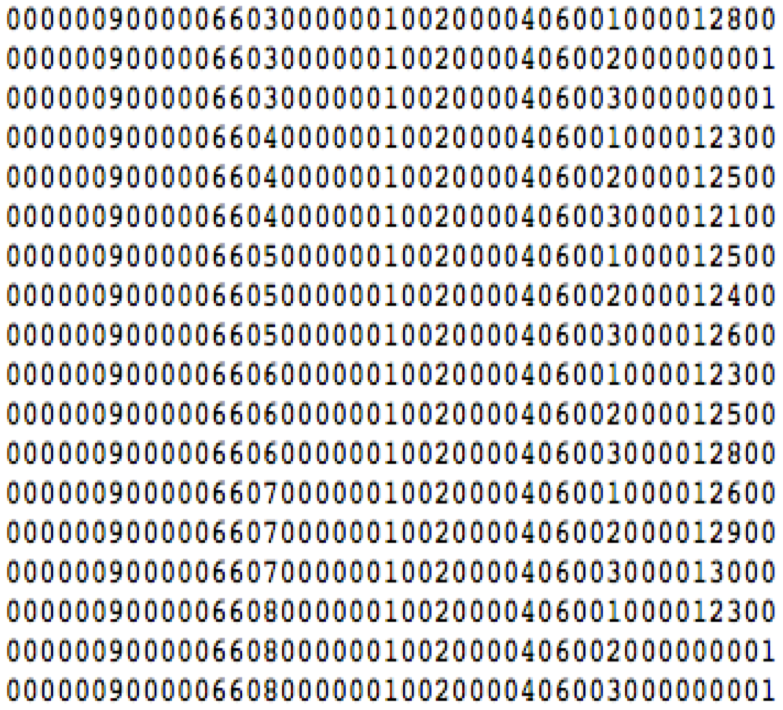
\includegraphics[width=3in]{/Users/jaylee/Desktop/thesis/img/ballot_image} \caption{Original ballot image data}\label{fig:ballot-image}
\end{figure}
In the ballot file, each voter is spread across three rows of data (one for each ranking). We use the \texttt{clean\_ballot()} function from our \texttt{rcv} R package (Lee \& Yancheff, 2019) to read in the data and cobine the ballot image with the lookup table. From this data we obtain the full ranked preference set of candidates (up to 3) from each voter (see Figure \ref{fig:cleaned-ballot}).
\begin{figure}
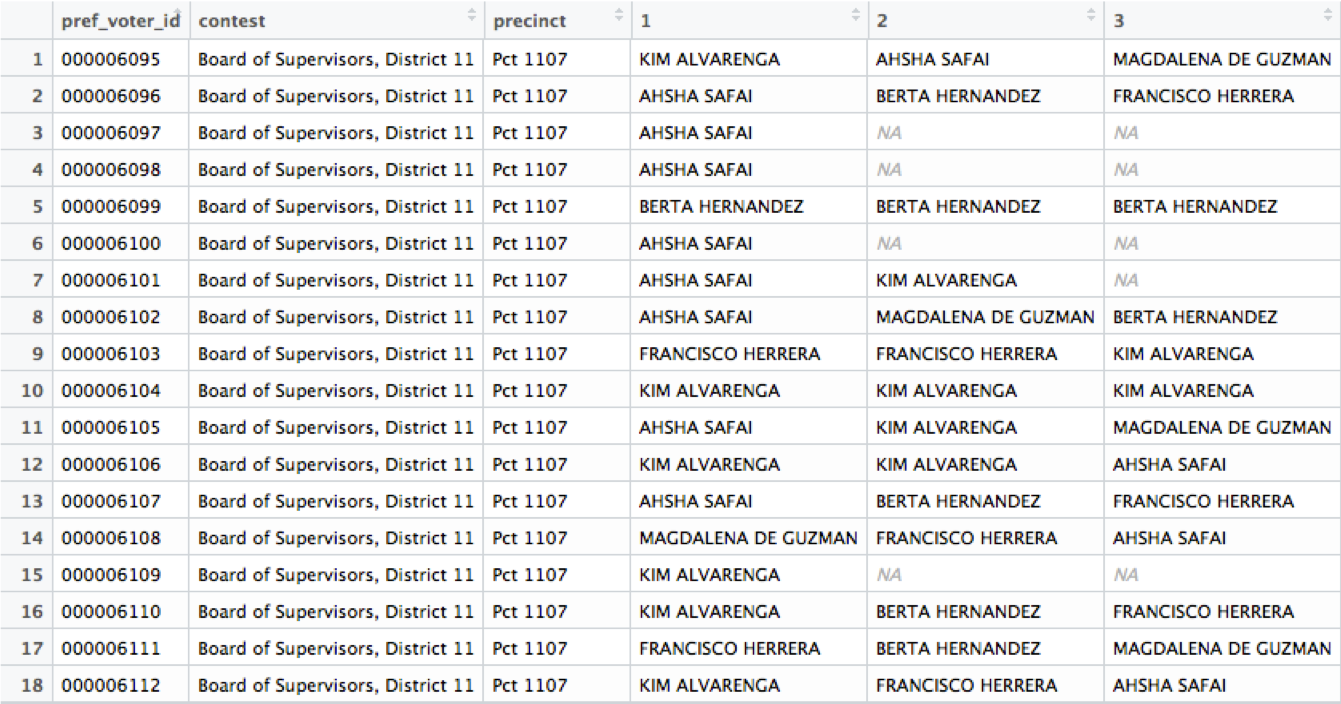
\includegraphics[width=6in]{/Users/jaylee/Desktop/thesis/img/cleaned_ballot} \caption{Cleaned RCV ballot}\label{fig:cleaned-ballot}
\end{figure}
Since the voter-level data is fully anonymized, we have no demographic information at the individual level. For any given voter, because the most identifying piece of information we have about them is their precinct, it is impossible to know any one voter's gender or ethnicity. To gain insight into these demographic trends, we instead aggregate up to the precinct level.

At the precinct level, we can now only study the rates of these ballot phenomena (as opposed to an individual's response). For example, in Precinct 1101, we see that 23.7\% of voters undervote. Rather than building a classification model (error / no error), we can now instead build regression models with a numerical dependent variable - the rate of ballot error. Moving up this level of abstraction does remove some granularity from the model (inference and prediction at the precinct level is less specific than at the individual level), but this is the least we can do that stil allows us to to access demographic information.

\hypertarget{demographic-data}{%
\subsection{Demographic data}\label{demographic-data}}

Now that we have precinct-level rates, we need to obtain precinct-level demographic information in order to build a model. Our source of demographic data is the 2012-2016 American Community Surveys (ACS) as part of the 2018 Census Planning Database ({\textbf{???}}). This data was chosen\footnote{Over the 2010 Census, which is also included in the Planning Database. While the Census has ``zero error'' since it's not a survey, it is also more out of date this late in the decade and didn't contain the same useful variables we were interested in.} because it contained demographic variables which we thought would be informative to our question: age, race and ethnicity, education, and poverty levels.

One consideration with this is that the voting population is not always representative of the general population. It might be more informative to obtain demographics about the voting population specifically, rather than the entire population of each precinct. However, the only information directly available about voters is their age (from the county voter registration file), and we consider the discontinuity introduced by using two different data sets for demographic information to be more of an issue than using a less accurate (but universal) census data set.

We also obtain a block group boundary shapefile from the Bureau ({\textbf{???}}).

\hypertarget{areal-interpolation}{%
\subsubsection{Areal Interpolation}\label{areal-interpolation}}

We now encounter a problem. Since census regions (block groups, tracts) are set by the federal government, and election precincts are set by San Francisco County\footnote{The city and county government are unified in this case, because the county comprises entirely of the city of San Francisco.}, the regions don't line up cleanly\footnote{There's no inherent reason that they should, it's just unfortunate for this study.} (see Figure \ref{fig:boundary-mismatch}). Given this mismatch, how do we obtain demographic estimates for our precincts?

Stated more generally: if we have a division of a geographic region and some set of properties on the divisions, how do we estimate measures of these properties for other possible divisions?
\begin{verbatim}
Reading layer `SF_DOE_Precincts_2017' from data source `/Users/jaylee/Desktop/thesis/raw_data/sf_precinct_shp' using driver `ESRI Shapefile'
Simple feature collection with 612 features and 11 fields
geometry type:  MULTIPOLYGON
dimension:      XY
bbox:           xmin: 5979386 ymin: 2085730 xmax: 6033437 ymax: 2130982
epsg (SRID):    NA
proj4string:    +proj=lcc +lat_1=37.06666666666667 +lat_2=38.43333333333333 +lat_0=36.5 +lon_0=-120.5 +x_0=2000000 +y_0=500000.0000000001 +datum=NAD83 +units=us-ft +no_defs
\end{verbatim}
\begin{verbatim}
Reading layer `gz_2010_06_150_00_500k' from data source `/Users/jaylee/Desktop/thesis/raw_data/ca_census_shp' using driver `ESRI Shapefile'
Simple feature collection with 23203 features and 8 fields
geometry type:  MULTIPOLYGON
dimension:      XY
bbox:           xmin: -124.4096 ymin: 32.53416 xmax: -114.1344 ymax: 42.00952
epsg (SRID):    4269
proj4string:    +proj=longlat +datum=NAD83 +no_defs
\end{verbatim}
\begin{verbatim}
Warning in st_centroid.sf(.): st_centroid assumes attributes are constant
over geometries of x
\end{verbatim}
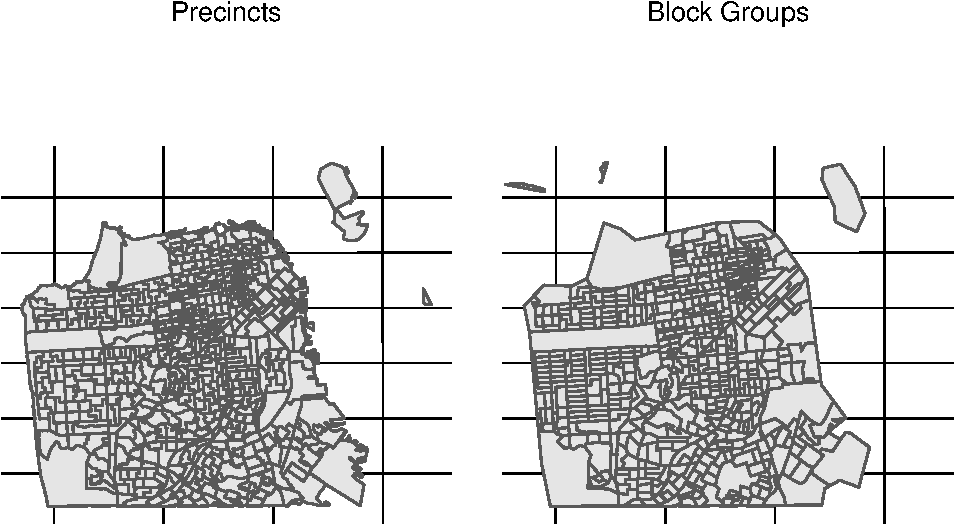
\includegraphics{thesis_files/figure-latex/boundary-mismatch-1.pdf}

One field of GIS (geographic information system) research that looks into this is called \emph{areal interpolation}. The goal of areal interpolation is to take a variable distributed over a set of ``source zones'' and estimate its distribution over a set of ``target zones'' (Schroeder, 2007). These two zoning systems must overlap at least partially to get any estimate for the target zones (e.g.~information about Oregon doesn't directly tell us anything about information in Washington, under any zoning system), but are incompatible in some way\footnote{A set of ``compatible'' zoning systems would be something like the US Census' hierarchical systems: multiple blocks are combined to make a block group, multiple block groups are combined into a census tract, etc. Since the areas overlap neatly, you can directly add together certain numbers (like population) from block groups to get a very accurate estimate for the census tract.}. When this is not possible, however, areal interpolation can help get parameter estimates for these incompatible areas.

Soem common types of areal interpolation are:
\begin{itemize}
\item
  Areal weighting, using the assumption that populations are distributed uniformly on a region.
\item
  Modified areal weighting, which creates a continuous map from region to region to better reflect changes in population density.
\item
  Target density weighting, which uses extra information about the target zones, typically population density, to increase accuracy (Schroeder, 2007).
\item
  Dasymetric mapping, which uses alternative data, also called \emph{ancillary data} to produce a continuous estimate of population density (Sleeter and Gould, 2008). Examples of ancillary data include land cover information, parcel classifications, and street locations.
\end{itemize}
In this work we will use areal weighting for our interpolation. The other methods above, while typically more accurate are infeasible under the constraints of the research\footnote{Mostly time limitations; see Conclusion section for further research ideas.}. The assumption of uniformity is not necessarily correct, but in an urban area such as San Francisco it is more accurate than an area like the entire state of California, with a large urban/rural spread.

\hypertarget{areal-weighting}{%
\subsubsection{Areal weighting}\label{areal-weighting}}

Areal weighting first makes the assumption that populations are distributed uniformly over a space. If Region X has 100 people and we split X in half spatially, then we assume that 50 people are in each half. This also applies to sub-populations: if Region X has 20 non-White Hispanic people, then we assume each half has 10 non-white Hispanic people. This type of data, counts that can be divided into sub-regions, is called \emph{spatially extensive} data. Extensive data is data that applies to an entire region, but not any given sub-region.

Conversely, data that applies to any given sub-region of a region is called \emph{spatially intensive}. Properties like population density are spatially intensive under the uniformity assumption, because the ratio of population to area does not change upon examining a sub-region. Percentages are also spatially intensive - considering the sub-population as above, the percentage of non-White Hispanic people in Region X (20 out of 100, 20\%) does not change when we look at one of the sub-regions (10 out of 50, 20\%).

We will use the following example case to illustrate the areal interpolation process. Suppose regions \(A\), \(B\), \(C\), and \(D\) are the source regions (each taking up a quadrant of the square), and regions \(X\), \(Y\), and \(Z\) are the target regions (each taking up a third of the square vertically). Further suppose that the boundaries of the source regions and target regions are fully coincident, that is \(A \cup B \cup C \cup D = X \cup Y \cup Z\)\footnote{This example ignores the case where the covered regions are not coincident, which is a possibility in general. In this research we enforce coincidence in our data, however.}.

In general, denote a source region by \(S_i\) (over index set \(I\)) and a target region by \(T_j\) (over index set \(J\)). For any region \(R\), denote the area of \(R\) by \(Area(R)\), the measure of a given extensive property of \(R\) by \(x_R\), and the measure of a given intensive property of \(R\) by \(y_R\). These measures are known in the source regions, but unknown in the target regions (hence, the interpolation). Denote an estimate of a quantity with a caret, e.g.~\(\widehat{y_{R}}\).

Say we want to estimate \(x_{T_j}\), the measure of the extensive property in region \(T_j\). For all \(j \in J\), we can estimate this property with
\[
\widehat{x_{T_j}} = \sum_{i \in I} \frac{Area(S_i \cap T_j)}{Area(S_i)} \cdot x_{S_i}
\]

For each source region, calculate the proportion of the region that lies inside the target region. These proportions are the weights to be multiplied by the source regions' properties. In the example case, consider target region \(X\):
\[
\widehat{x_X} = \frac{Area(A \cap X)}{Area(A)} \cdot x_{A} + \frac{Area(B \cap X)}{Area(B)} \cdot x_{B} + 0 + 0 = \frac{2}{3}(x_A + x_B)
\]

Since \(A\) and \(B\) each have \(2/3\) of their area inside target region \(X\), we estimate that 2/3 of the extensive quantity \(x_A\) is inside region \(X\) (similarly for \(x_B\)). Adding these together gives us an estimate \(\widehat{x_X}\).

For intensive properties, the process is slightly different. For all \(j \in J\), we can estimate an intensive property \(y_{T_j}\) with
\[
\widehat{y_{T_j}} = \sum_{i \in I} \frac{Area(S_i \cap T_j)}{Area(T_j)} \cdot x_{S_i}
\]

Since the intensive property isn't ``divisible'' within a region, we instead take a weighted average of the component source regions of the target region, where each component is weighted by the amount of the target region it takes up. Again considering target region \(X\):
\[
\widehat{y_X} = \frac{Area(A \cap X)}{Area(X)} \cdot y_{A} + \frac{Area(B \cap X)}{Area(X)} \cdot y_{B} + 0 + 0 = \frac{1}{2}(y_A + y_B)
\]

Since \(A\) and \(B\) each take up half of target region \(X\), each of them gets weighted by half before being added to get the estimate of \(y_X\).

To validate the application of this method to the data at hand, we can visually compare the spatial distribution of a variable before the interpolation to its distribution after the interpolation.
\begin{figure}
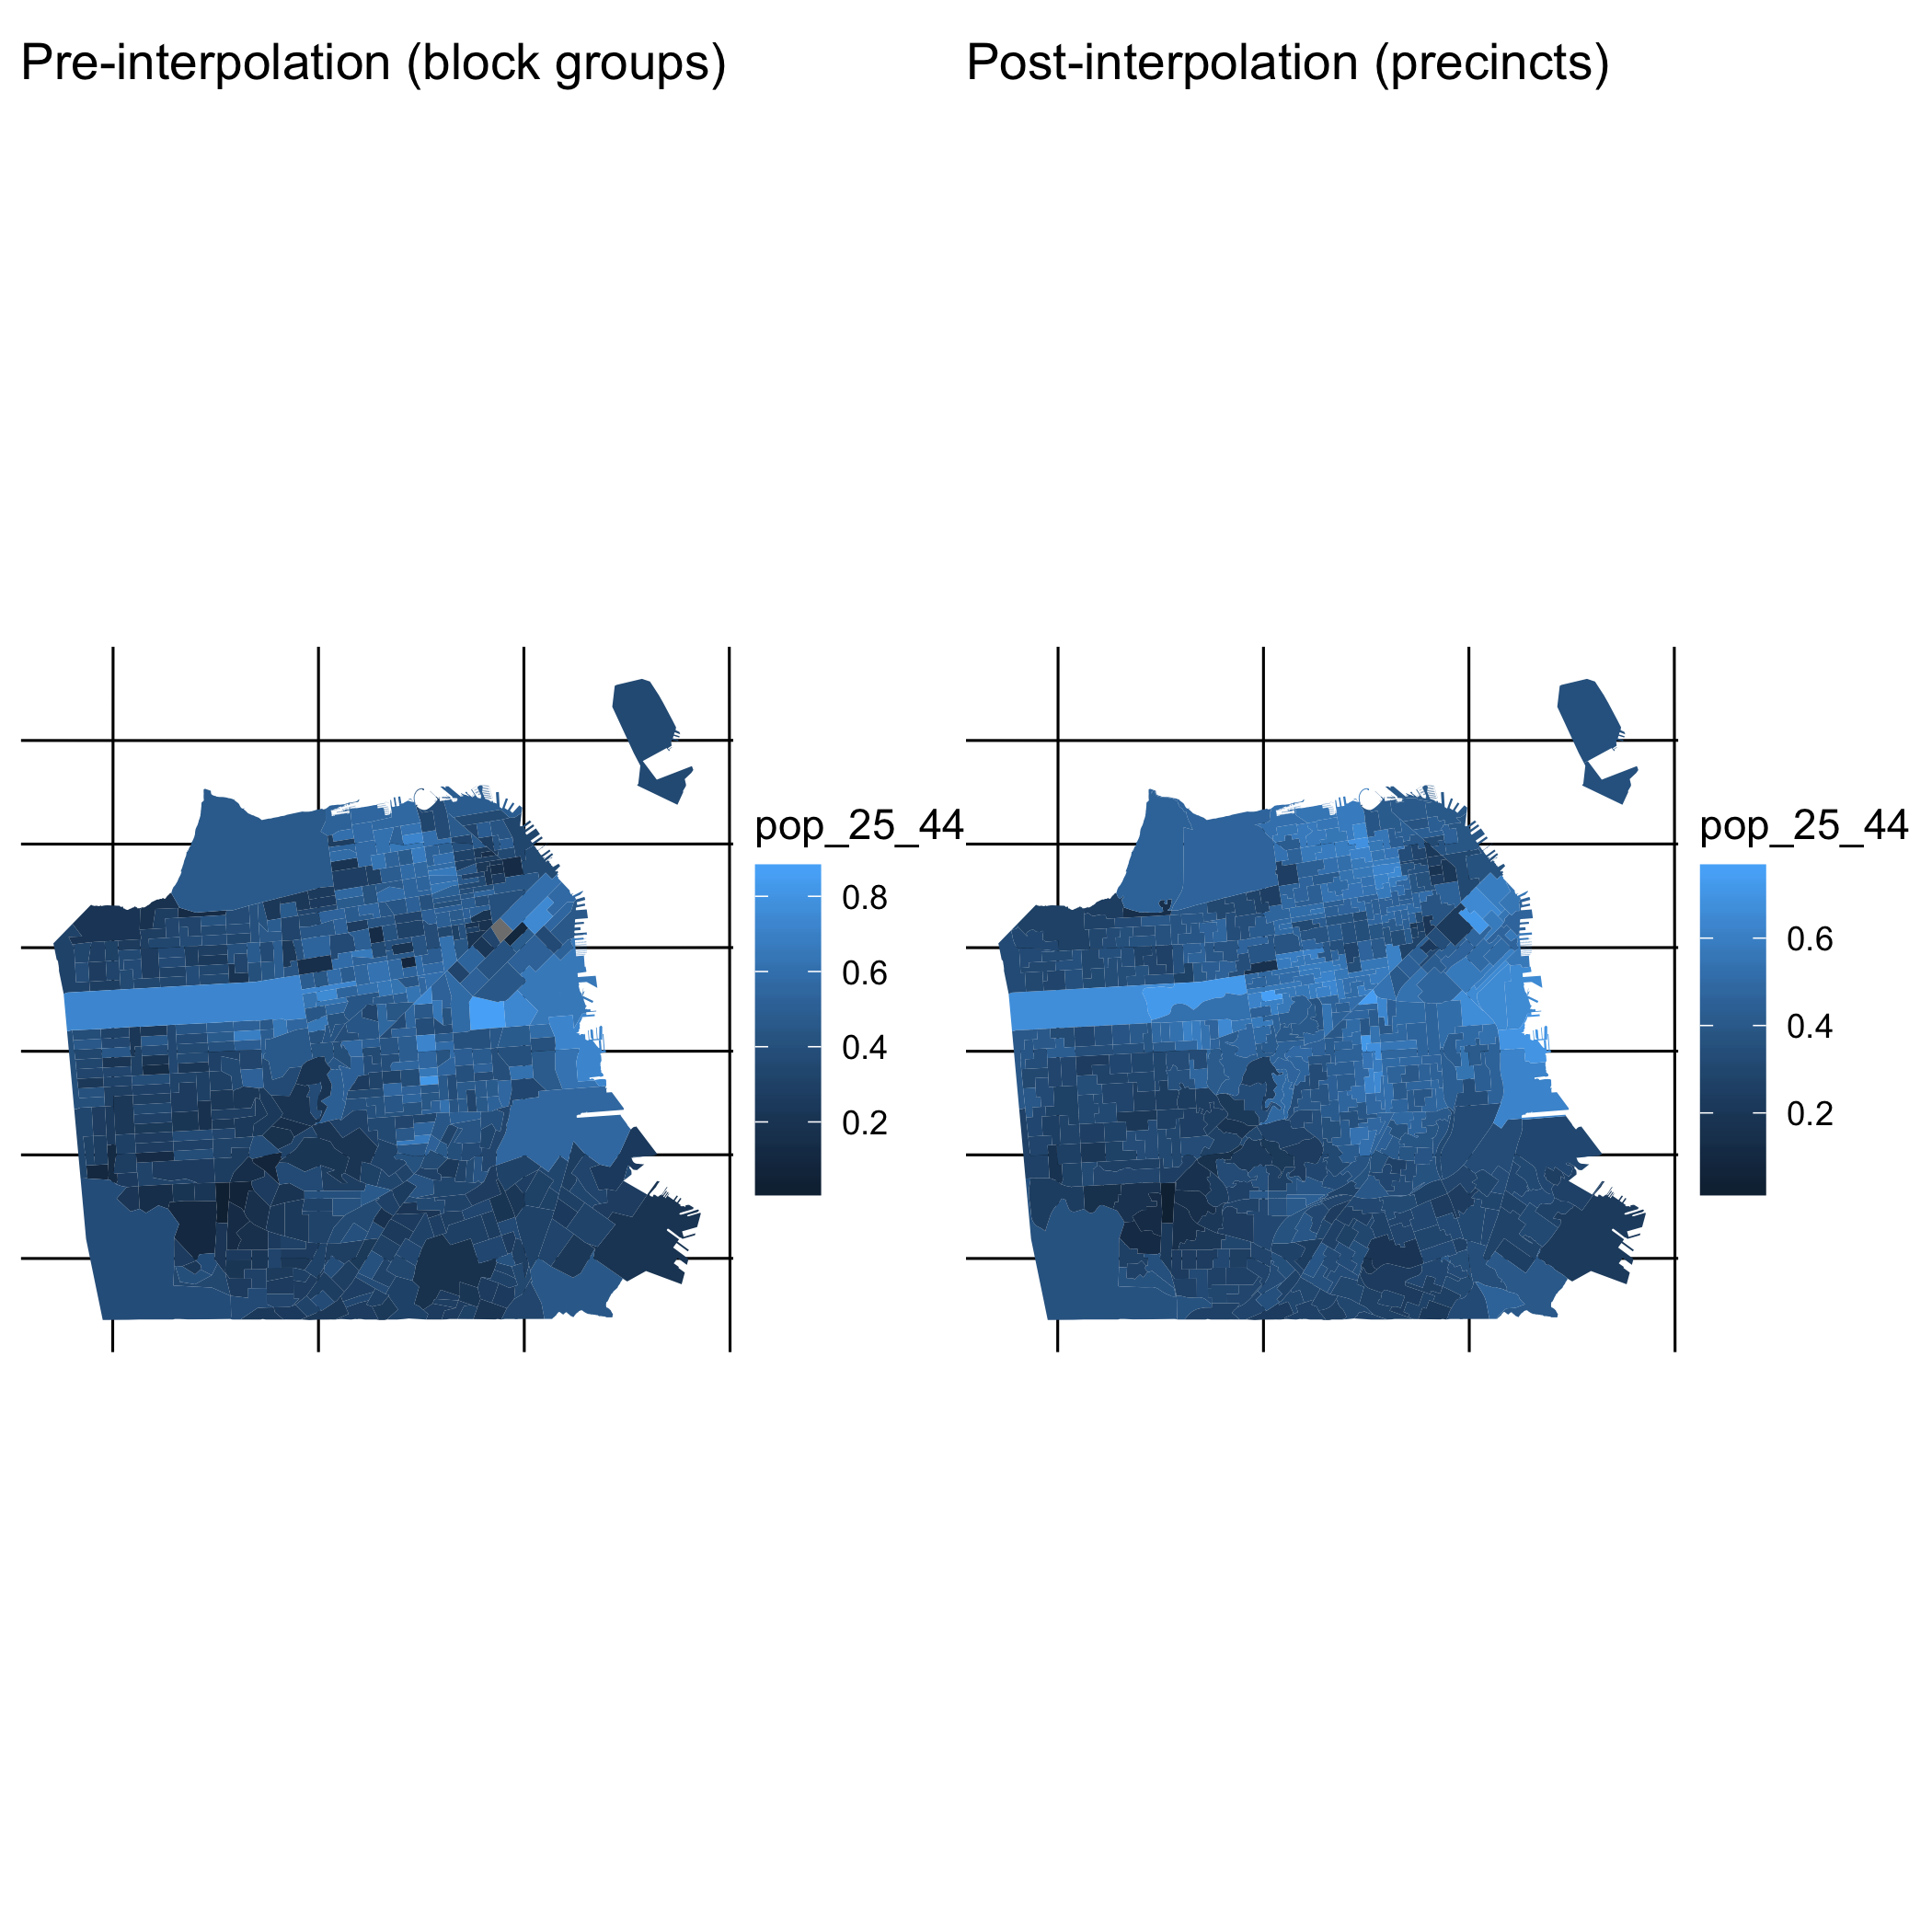
\includegraphics[width=28.64in]{/Users/jaylee/Desktop/thesis/img/interpolation_check} \caption{Proportion of non-Hispanic Asian residents}\label{fig:unnamed-chunk-4}
\end{figure}
\hypertarget{interpolation---counts-vs.-percentages}{%
\subsubsection{Interpolation - counts vs.~percentages}\label{interpolation---counts-vs.-percentages}}

One consideration in the data preparation stage was whether to use counts or percentages as input for the regression. The census data contains total population in a region, as well as a count and percentage for a given variable (say people between the ages of 25 and 44). The percentage can equivalently be calculated by dividing the count by the population. After performing the areal interpolation on the data, I ran this percentage calculation again to double check that it lined up with the reported percentages (post-interpolation). My intuition was that these steps should be commutative - calculating a percentage and then interpolating should have the same result as interpolating and then calculating the percentage. This was not the case, however - in the variable for population between 25 and 44, the error between these two methods ranged from -12 to 26 percentage points.
\begin{figure}
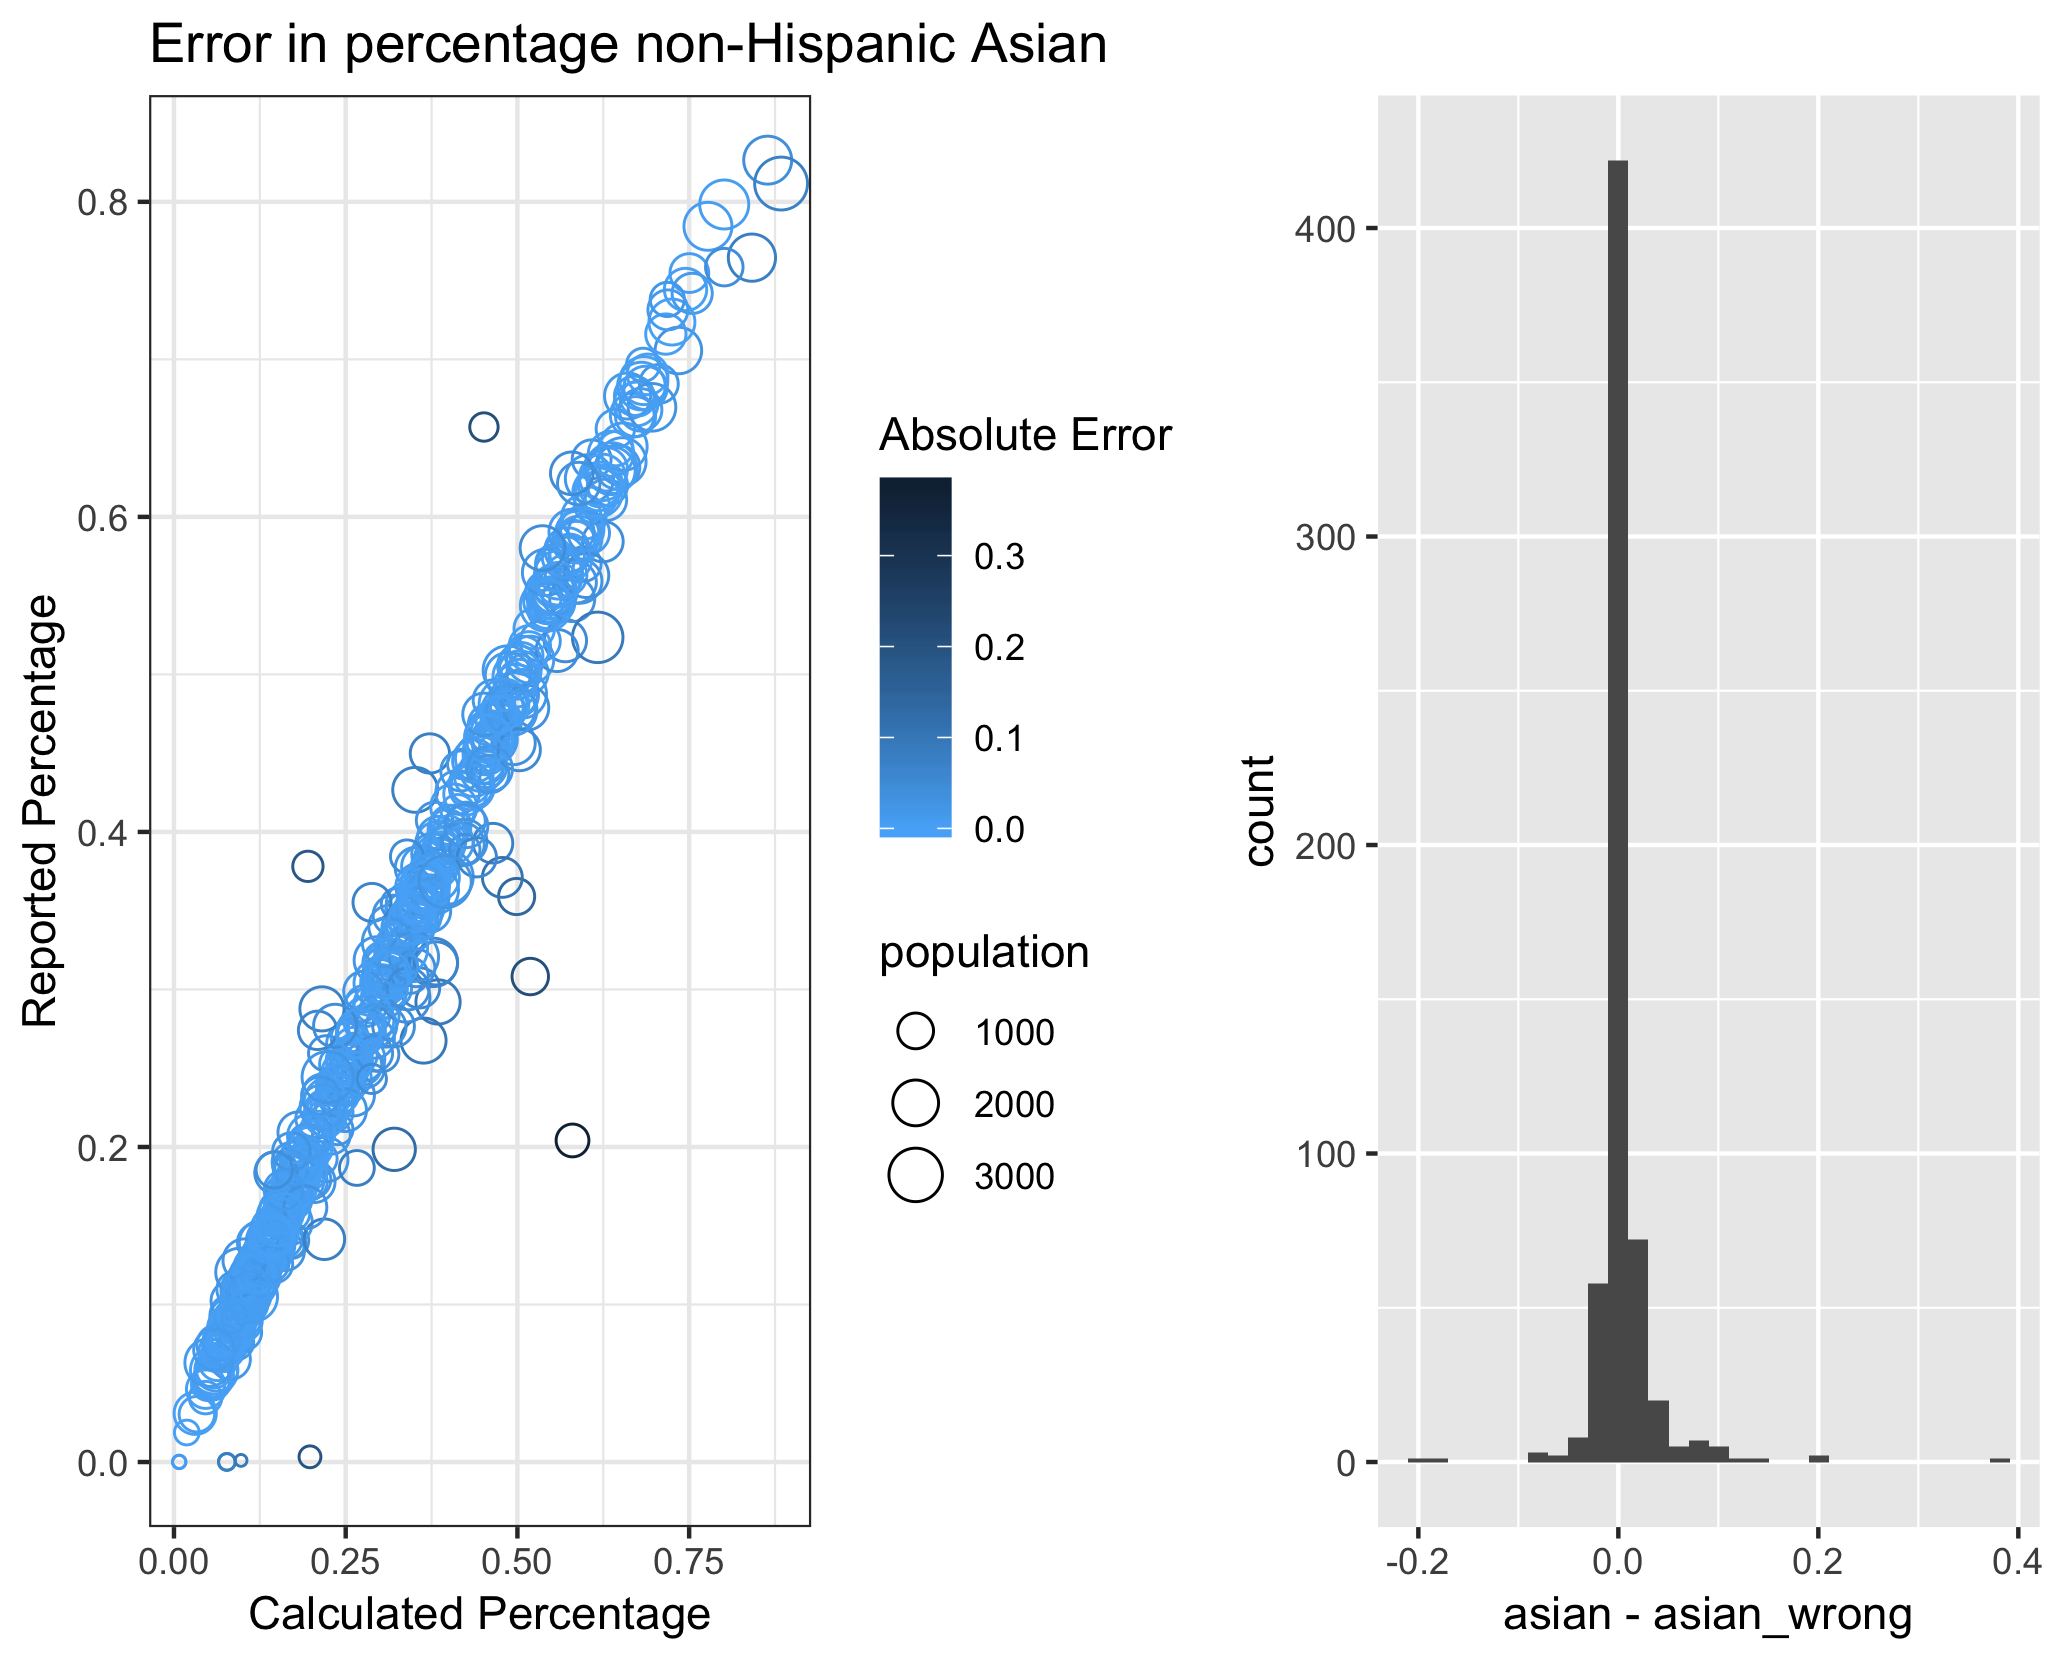
\includegraphics[width=28.64in]{/Users/jaylee/Desktop/thesis/img/intensive_error} \caption{Sample error in intensive interpolation}\label{fig:unnamed-chunk-5}
\end{figure}
As it turns out, these steps are not commutative in this way, and the observed error is mostly a function of the weighting between different steps in the process. For example, consider a simple case: suppose source regions A and B are fully contained in target region X, and split X in half. Let the number of people between 25 and 44 in A be 4 (out of 10 total) and in B be 3 (out of 5 total). Taking the percentages first gives us a proportion of 0.4 in A and 0.6 in B. Using the intensive interpolation method on these proportions, both are weighted by the amount of X that the region takes up (half, in each case) and added, so the average weighted by area is 0.5. Conversely, using the extensive interpolation method on the count and popuation, we see that X has 7 people between 25 and 44 (out of 15 total). Taking the percentage, we see that the proportion of this variable in X is \textasciitilde0.47.

In short, the ``calculating proportion'' and ``areal interpolation'' steps are NOT commutative, because of the differences in weights when using intensive vs.~extensive interpolation methods. Both are calculating a weighted mean of sorts, but the former is weighting by \textbf{area}, while the latter is weighting by \textbf{population}. In this case we see that the latter is more accurate - source regions with more people should have greater impact on the estimated measures in target regions, because the variables we are dealing with are human-centered rather than space-centered. As such, for this study we will interpolate only the count data (population, numbers of people for each measured variable) and then calculate proportions in the target regions after the interpolation. These proportions are better suited to the regression to ensure that variables are of the same scale and we can compare coefficient estimates.

\hypertarget{boundary-mismatch}{%
\subsubsection{Boundary mismatch}\label{boundary-mismatch}}

A further issue appears - just like the precinct and census boundaries don't line up because they come from different sources, the outside boundaries of the precinct and census files don't line up. The census boundaries have a lower resolution on the whole than then precinct boundaries. This leads to issues when performing the areal interpolation, because parts of a census boundary that are outside of a precinct will be dropped and cause an underestimate of the true measure of the variables. We address this by bounding both files to only consider the space that is contained in both\footnote{No census tracts were fully removed in this process, but this causes one precinct, Precinct 9900, to be cut off. However, this precinct is a semi-exclave of the county on Alameda Island, across the San Francisco Bay. Since this land, an undeveloped former naval air base, is uninhabited (Levi, 2018) its removal does not impact our results.}. Since we are dealing with a fundamental unit of people instead of space, this ensures that every person is counted, and changes some of the spatial weights calculated. The assumption here is that any region which is only contained in one of the files (precincts without census, or census without precincts) has zero population, because every person should be contained in both a precinct and a census region.
\begin{figure}
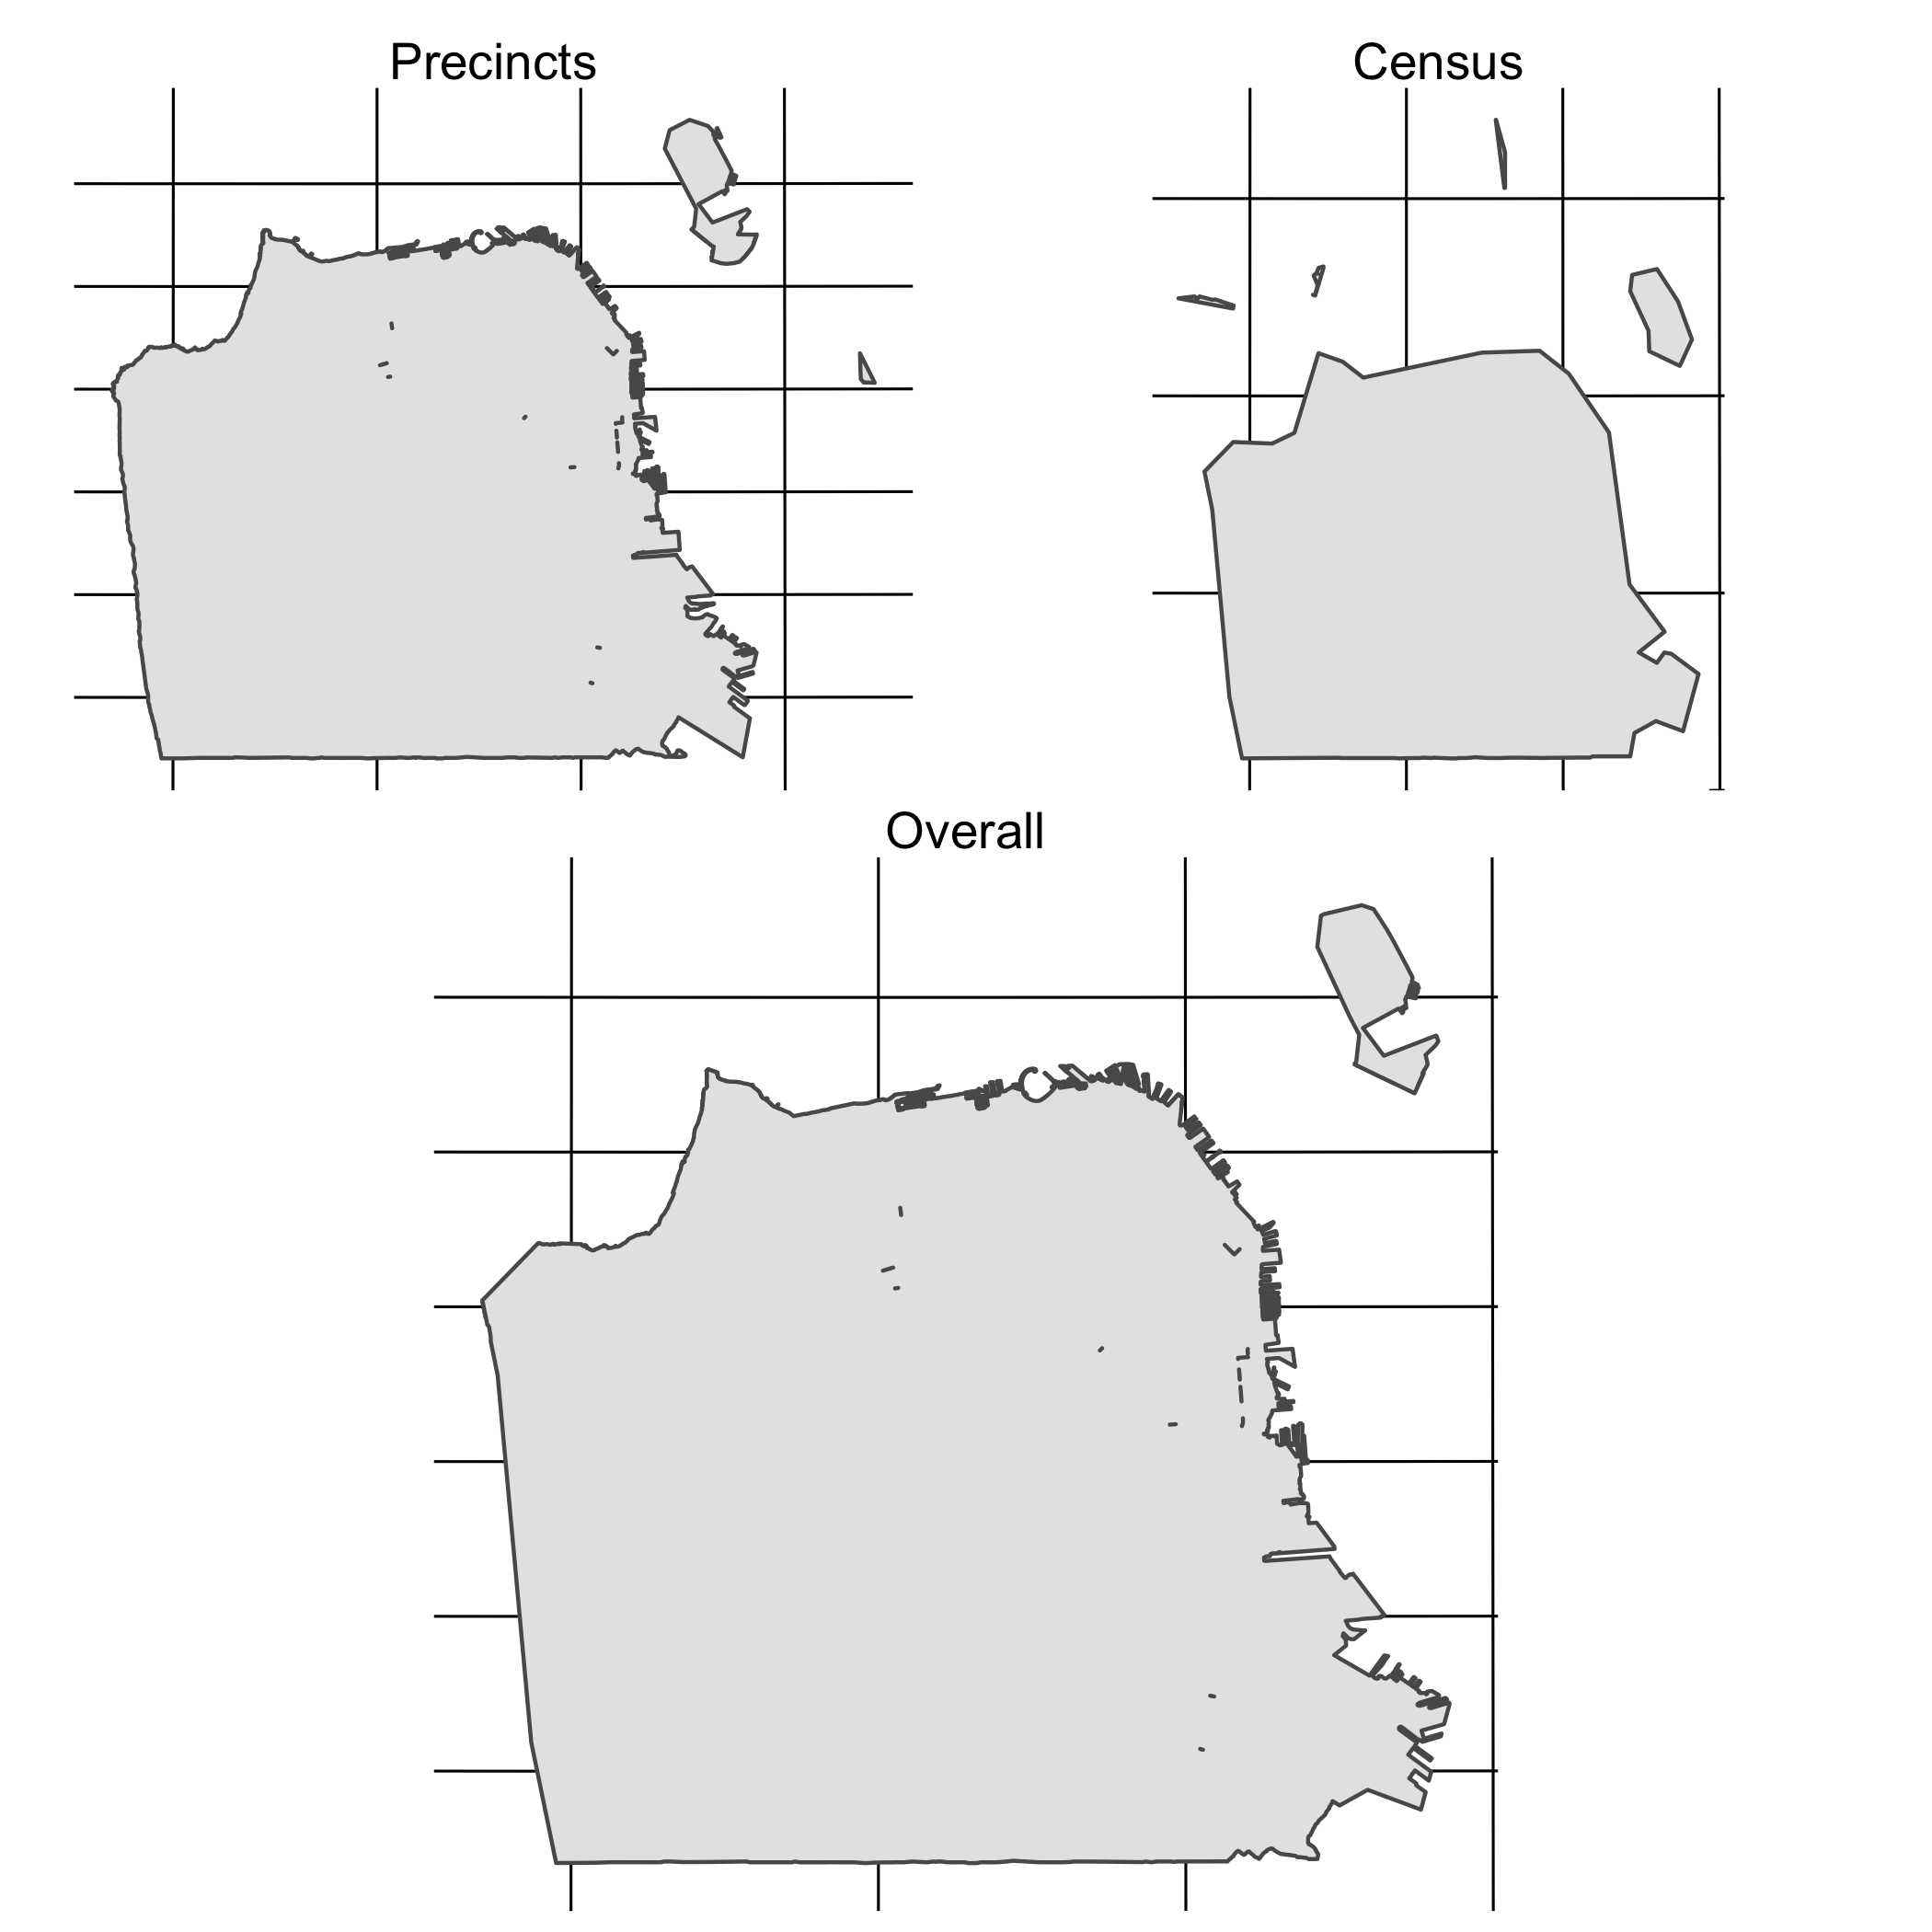
\includegraphics[width=29.17in]{/Users/jaylee/Desktop/thesis/img/boundary_intersection} \caption{Boundary intersection between shapefiles}\label{fig:unnamed-chunk-6}
\end{figure}
This plot\footnote{The plots were clipped to display the same area. There are some extra islands out of range on the precinct and census maps that are not shown.} displays the result of this intersection between the two regions. The impact on the census tracts is quite visible - notably the eastern coastline is much more defined, and the gap in Treasure Island (the large island off the northeastern shore) appears. The impact on the precinct boundaries is less apparent, but still there - foe example, in the southeastern corner it is visible how the angles in the precinct boundary have softened to the more rounded final shape.

Below is a comparison of the original shapefiles\footnote{The original census regions contained the Farallon Islands, which have been removed from this plot because they are uninhabited, 30 miles into the Pacific Ocean, and messed up the scale of the graph.} (including all divisions) to the bounded versions.
\begin{figure}
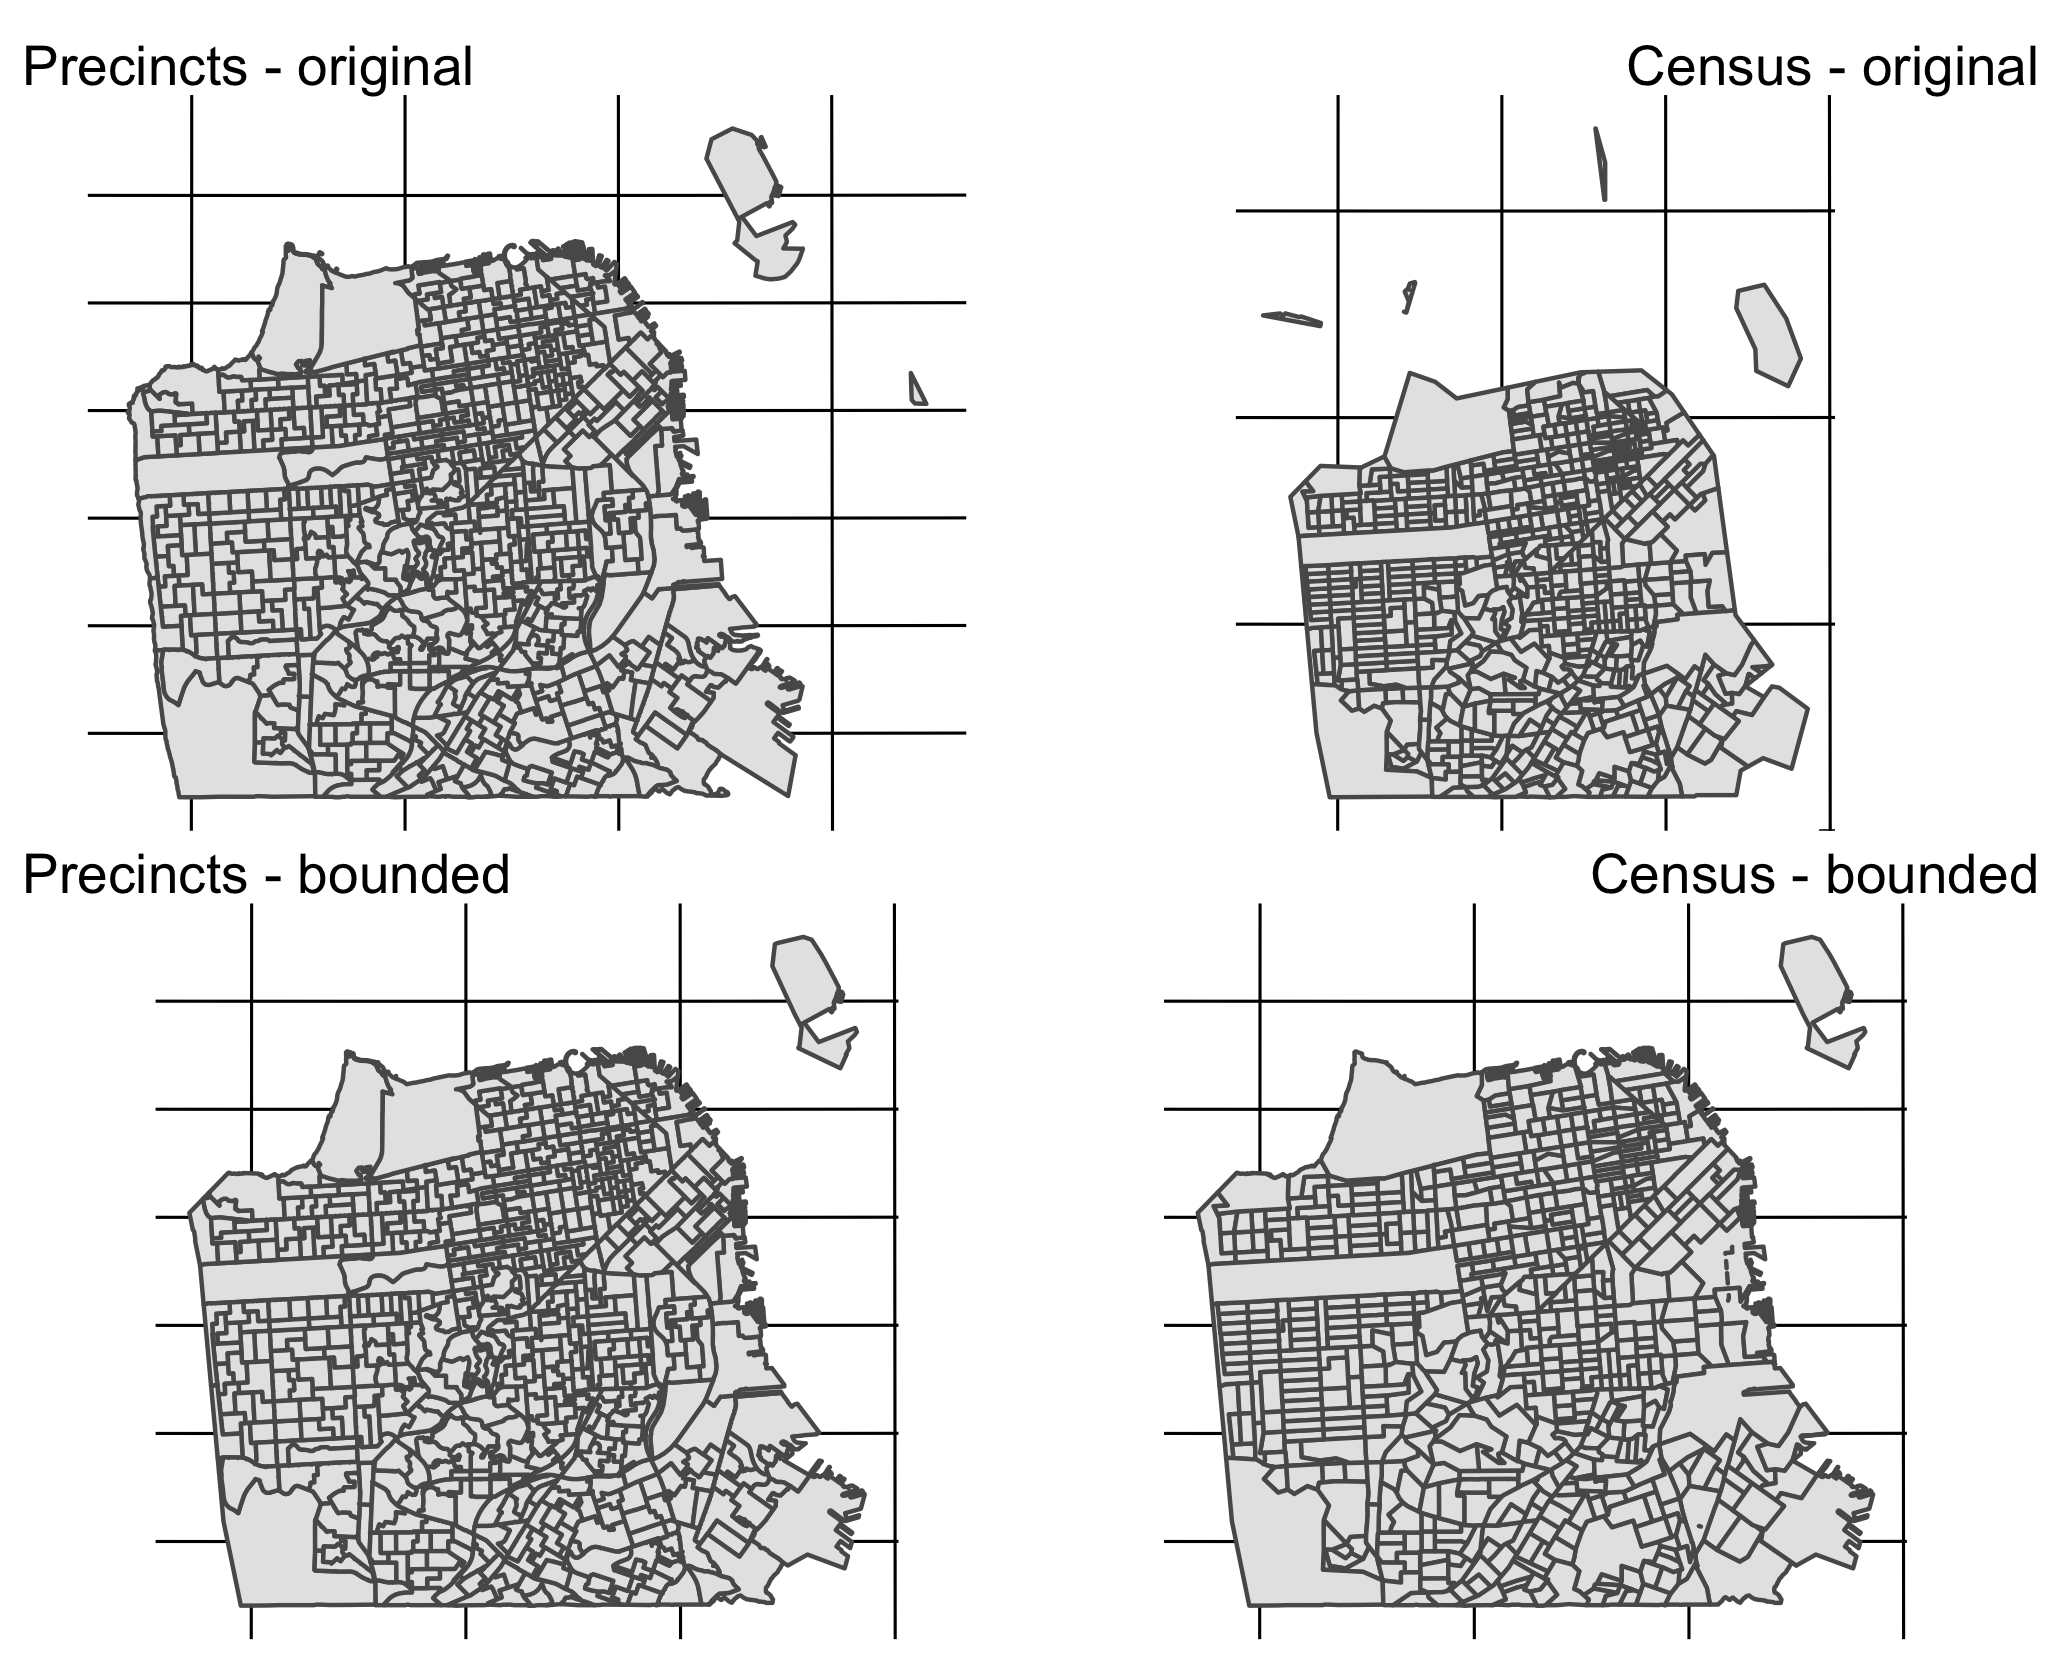
\includegraphics[width=28.64in]{/Users/jaylee/Desktop/thesis/img/clipped_internals} \caption{Original versus bounded shapefiles}\label{fig:unnamed-chunk-7}
\end{figure}
\hypertarget{precinct-consolidation}{%
\subsubsection{Precinct Consolidation}\label{precinct-consolidation}}

One peculiarity in San Francisco is the combination of certain precincts during elections. California state law allows for counties to ``consolidate'' precincts with low numbers of registered voters during an election. This eases administration by not requiring counties to set up and staff a full polling place in a precinct with few voters, while still giving voters a physical polling location in their approximate area\footnote{This method of precinct consolidation may change with the 2018 California Voter's Choice Act, which lets counties (except for Los Angeles County) move fully to vote-by-mail in combination with voting centers (California Senate Bill 450).}. While San Francisco does this less often than other counties, there are still some precincts that are consolidated each election.

The areal interpolation process produces demographic estimates for areas in the map, however, which are non-consolidated. This causes a mismatch: we have demographic data for individual precincts, but election data for the consolidated precincts. To address this issue, we have split the election data (a count of overvotes and undervotes) in the consolidated precincts into their two component precincts. This split is weighted by the population of each precinct in 2010\footnote{The most simple weight would be 50-50 for each split, but this is inaccurate for many of these precincts: see the gap in the weights for Pct 7527/7528. The flaw in this method was discovered after calculating turnout of over 1000\% for Precinct 7527\ldots{}}. For example, suppose Precinct X/Y had 100 undervotes, the population of Precinct X in 2010 was 325, and the population of Precinct Y in 2010 was 175. Then the ``population split'' between X and Y is 65\%-35\%, and we adjust the undervotes accordingly: Precinct X should have 65 of the 100 undervotes, and Precinct Y should have the remaining 35.

Examples of this in the data are below. The first table is the initial data, with full consolidated counts doubled in the precincts (and thus doubled across rows), and the second table is the data with proper weights applied. Note that this is 6 out of the 12 total precincts that get combined into 6 double precincts.
\begin{longtable}{llrrrr}
\caption[Consolidated Precincts - Original]{\label{tab:unnamed-chunk-8}Consolidated Precincts - Original Data}\\
\toprule
Election Pct. & Pct. Number & Over & Not over & Under & Not under\\
\midrule
Pct 1104/1105 & 1104 & 1 & 455 & 133 & 323\\
Pct 1104/1105 & 1105 & 1 & 455 & 133 & 323\\
Pct 7509/7511 & 7511 & 0 & 491 & 151 & 340\\
Pct 7509/7511 & 7509 & 0 & 491 & 151 & 340\\
Pct 7527/7528 & 7527 & 2 & 392 & 119 & 275\\
\addlinespace
Pct 7527/7528 & 7528 & 2 & 392 & 119 & 275\\
\bottomrule
\end{longtable}
\begin{longtable}{llrrrrr}
\caption[Consolidated Precincts - Weighted]{\label{tab:unnamed-chunk-9}Consolidated Precincts - Weighted Data}\\
\toprule
Election Pct. & Pct. Number & Weight & Over & Not over & Under & Not under\\
\midrule
Pct 1104/1105 & 1104 & 0.4060452 & 0 & 185 & 54 & 131\\
Pct 1104/1105 & 1105 & 0.5939548 & 1 & 270 & 79 & 192\\
Pct 7509/7511 & 7511 & 0.7438036 & 0 & 365 & 112 & 253\\
Pct 7509/7511 & 7509 & 0.2561964 & 0 & 126 & 39 & 87\\
Pct 7527/7528 & 7527 & 0.0129859 & 0 & 5 & 2 & 4\\
\addlinespace
Pct 7527/7528 & 7528 & 0.9870141 & 2 & 387 & 117 & 271\\
\bottomrule
\end{longtable}
\hypertarget{calculating-overundervote-info}{%
\section{Calculating over/undervote info}\label{calculating-overundervote-info}}

Move this further up to the section where you talk about that? Or move that down because it lines up with the actual process

RCV package (with Matthew)
Data from the city elections board
Data is missing some ballots that had to be hand-counted because it spits out straight from the machine, so this won't necessarily match the official reports.

Data comes in in weird double file form, then gets cleaned up and looks like this.
\begin{longtable}{lllll}
\caption{\label{tab:unnamed-chunk-10}Processed Ballot Image}\\
\toprule
Contest & Voter ID & 1 & 2 & 3\\
\midrule
Mayor & 000012886 & JANE KIM & ELLEN LEE ZHOU & MARK LENO\\
Mayor & 000012887 & JANE KIM & ANGELA ALIOTO & RICHIE GREENBERG\\
Mayor & 000012888 & JANE KIM & LONDON BREED & ANGELA ALIOTO\\
Mayor & 000012889 & JANE KIM & LONDON BREED & ANGELA ALIOTO\\
Mayor & 000012890 & LONDON BREED & JANE KIM & MARK LENO\\
\addlinespace
Mayor & 000012891 & MARK LENO & LONDON BREED & ANGELA ALIOTO\\
Mayor & 000012892 & MARK LENO & LONDON BREED & JANE KIM\\
Mayor & 000012893 & MARK LENO & ANGELA ALIOTO & MICHELLE BRAVO\\
Mayor & 000012894 & LONDON BREED & ANGELA ALIOTO & MARK LENO\\
Mayor & 000012895 & ELLEN LEE ZHOU & MICHELLE BRAVO & JANE KIM\\
\bottomrule
\end{longtable}
In this view, an overvote in a ranking appears as \texttt{NA} in that ranking

\hypertarget{regressions}{%
\section{Regressions}\label{regressions}}

Methods for regression:
\begin{itemize}
\tightlist
\item
  Linear ?
  \begin{itemize}
  \tightlist
  \item
    Pretty simple honestly
  \end{itemize}
\item
  Logistic with the ``binomial-style'' input data
  \begin{itemize}
  \tightlist
  \item
    This is more useful because our output (rate) is 0-1 limited.
  \item
    It also overweights precincts with more people - is this good? (Ask Heather)
  \end{itemize}
\item
  For whatever goes in, I need to pick a better model selection method.
\item
  Also test / train data set
\item
  Cross-validation?
\item
  ex post facto model validation! The residual plots and all that. This could also go in the results section.
\item
  Weights based on population? Based on number of voters? weights for future research maybe
\item
  surveyglm/svyglm package to do this weighting
\item
  Graphic of precinct turnout
\item
  Regression for voter turnout AT ALL and these demographics
\item
  Histogram just for how much undervoting or overvoting there is
\item
  Zero-inflated? Because there's so many zeroes and we're technically dealing with a census on the voting end (future research, ``I'm aware of this'')
\end{itemize}
\hypertarget{demo-results}{%
\chapter{Demographic analysis results}\label{demo-results}}

For the following models, I use variables taken from the US Census 2018 Planning Database\footnote{All descriptions taken from the Planning Database as well.}, estimated for the election precincts through the areal interpolation method. All data is self-reported through the Census process\footnote{In regards to the \texttt{female} variable: the Census specifically asks about binary sex; there are currently no questions about gender identity.}. A description of these variables is in the \protect\hyperlink{appendix}{Appendix}.

\hypertarget{modeling-turnout}{%
\section{Modeling turnout}\label{modeling-turnout}}
\begin{verbatim}
`stat_bin()` using `bins = 30`. Pick better value with `binwidth`.
\end{verbatim}
\begin{figure}
\centering
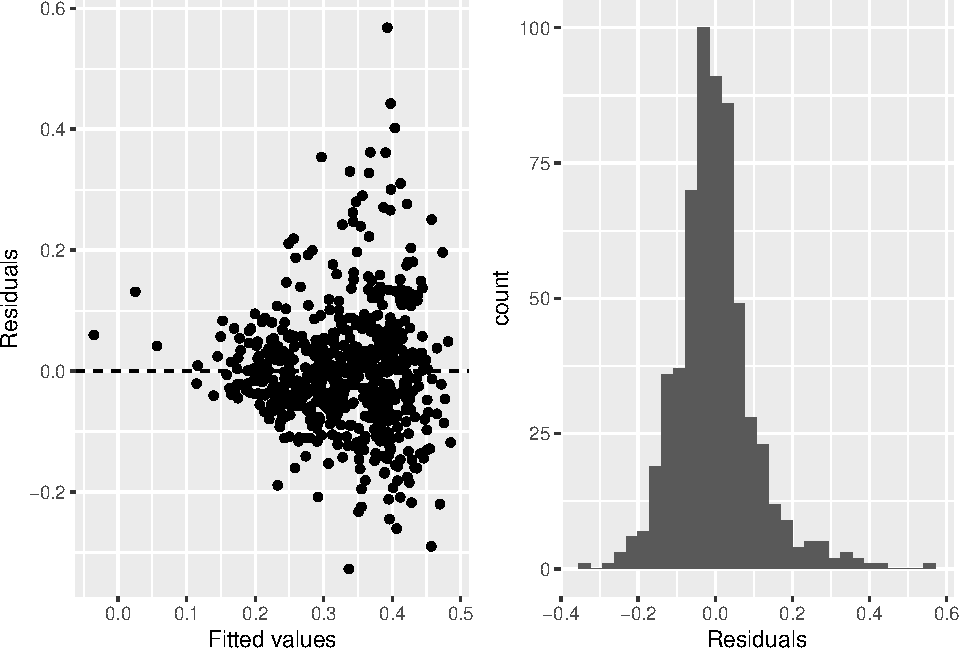
\includegraphics{thesis_files/figure-latex/unnamed-chunk-13-1.pdf}
\caption{\label{fig:unnamed-chunk-13}Observed turnout rate by precinct}
\end{figure}
With an adjusted \(R^2\) value of 0.3731852, the best linear model we found for predicting turnout\footnote{From the dataset, we removed one outlier with a turnout rate of 124\%, Precinct 7024. We believe this is a particlarly egregious inaccuracy in the interpolation process of calculating population. The gaps in the map above and following maps are Golden Gate Park (to the northwest), Crocker-Amazon Playground and John McLaren Park (to the south), and our removed precinct 7024 (to the southeast).} included variables for both age and education. A district having more young people (18-24) was negatively correlated with turnout, while having more middle-aged and college-educated people was positively correlated with turnout. This is consistent with general literature on voter turnout - young people vote less, and the better educated vote more.
\begin{longtable}{lrrrr}
\caption[Linear turnout model]{\label{tab:unnamed-chunk-14}Linear model for RCV voter turnout}\\
\toprule
term & estimate & std.error & statistic & p.value\\
\midrule
Intercept & 0.0807417 & 0.0295384 & 2.733451 & 0.0064529\\
pop\_18\_24 & -0.4125588 & 0.0686999 & -6.005235 & 0.0000000\\
pop\_45\_64 & 0.2920957 & 0.0741414 & 3.939711 & 0.0000912\\
college & 0.3534835 & 0.0230788 & 15.316360 & 0.0000000\\
\bottomrule
\end{longtable}
\begin{verbatim}
`stat_bin()` using `bins = 30`. Pick better value with `binwidth`.
\end{verbatim}
\begin{figure}
\centering
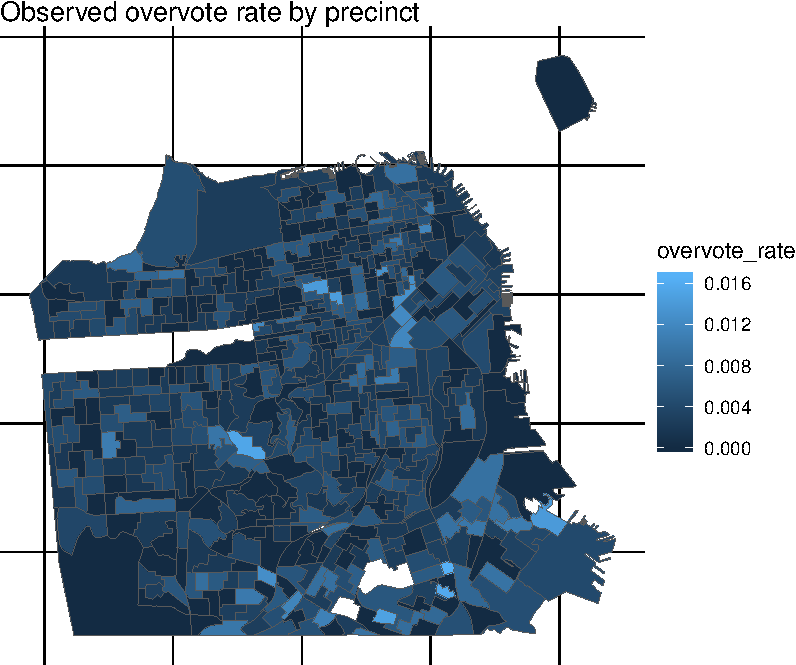
\includegraphics{thesis_files/figure-latex/unnamed-chunk-14-1.pdf}
\caption{\label{fig:unnamed-chunk-14}Linear turnout model validation}
\end{figure}
Logistic -

\hypertarget{modeling-overvoting}{%
\section{Modeling overvoting}\label{modeling-overvoting}}
\begin{verbatim}
`stat_bin()` using `bins = 30`. Pick better value with `binwidth`.
\end{verbatim}
\begin{figure}
\centering
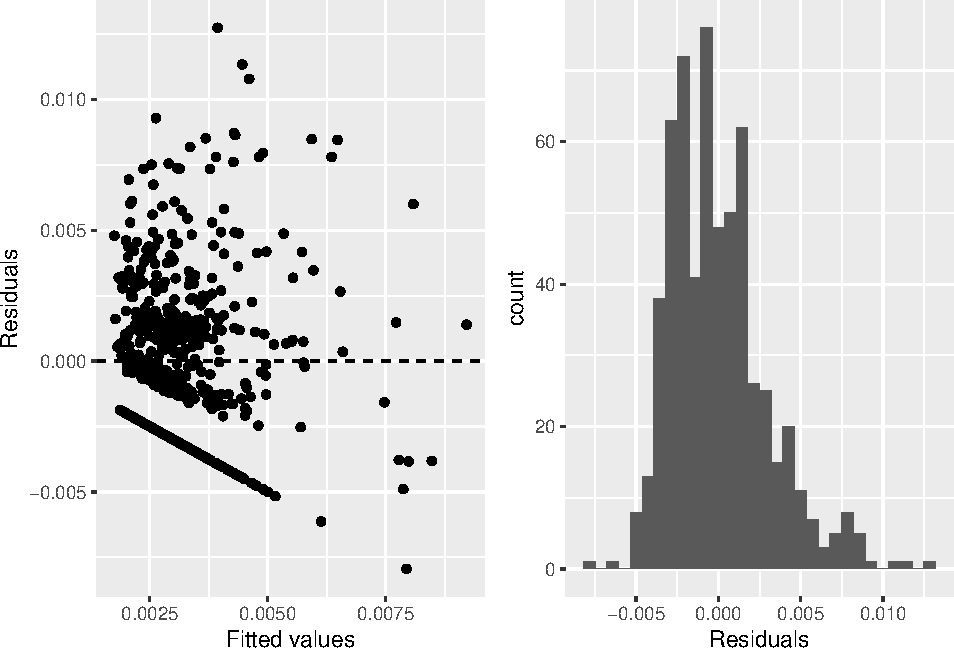
\includegraphics{thesis_files/figure-latex/unnamed-chunk-15-1.pdf}
\caption{\label{fig:unnamed-chunk-15}Observed overvote rate by precinct}
\end{figure}
With an adjusted \(R^2\) value of 0.1102897, the best linear model we found for predicting overvoting included variables for both race and education. A district being more African-American was positively correlated with overvoting, while having more college-educated people was negatively correlated with overvoting.
\begin{longtable}{lrrrr}
\caption[Linear overvote model]{\label{tab:unnamed-chunk-16}Linear model for overvoting in RCV}\\
\toprule
term & estimate & std.error & statistic & p.value\\
\midrule
Intercept & 0.0042211 & 0.0004209 & 10.027963 & 0.00e+00\\
black & 0.0092200 & 0.0016453 & 5.603925 & 0.00e+00\\
college & -0.0027021 & 0.0006421 & -4.207959 & 2.97e-05\\
\bottomrule
\end{longtable}
\begin{verbatim}
`stat_bin()` using `bins = 30`. Pick better value with `binwidth`.
\end{verbatim}
\begin{figure}
\centering
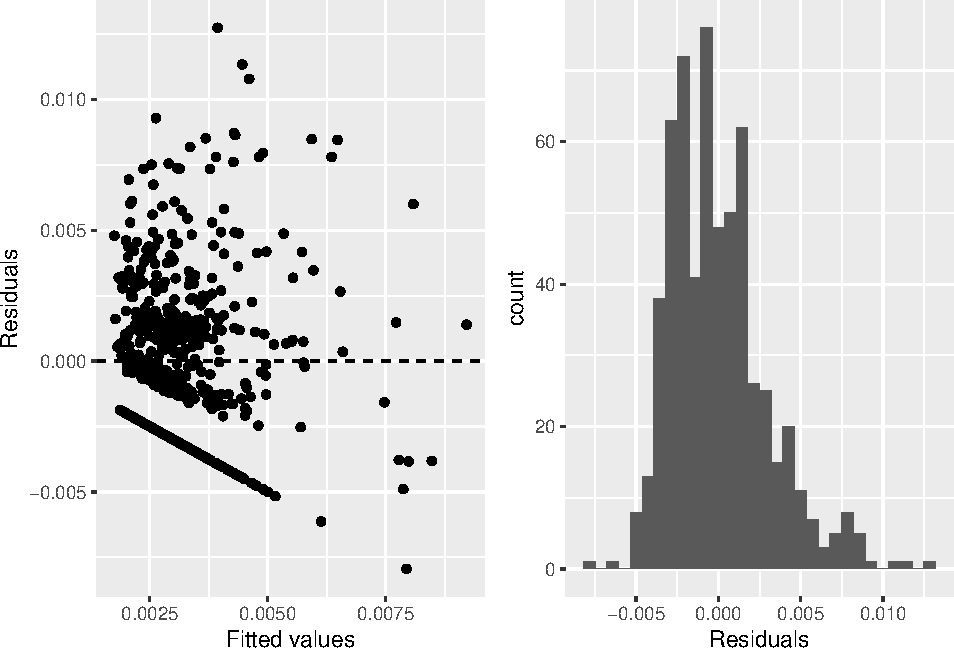
\includegraphics{thesis_files/figure-latex/unnamed-chunk-16-1.pdf}
\caption{\label{fig:unnamed-chunk-16}Linear overvote model validation}
\end{figure}
Logistic

\hypertarget{modeling-undervoting}{%
\section{Modeling undervoting}\label{modeling-undervoting}}
\begin{verbatim}
`stat_bin()` using `bins = 30`. Pick better value with `binwidth`.
\end{verbatim}
\begin{figure}
\centering
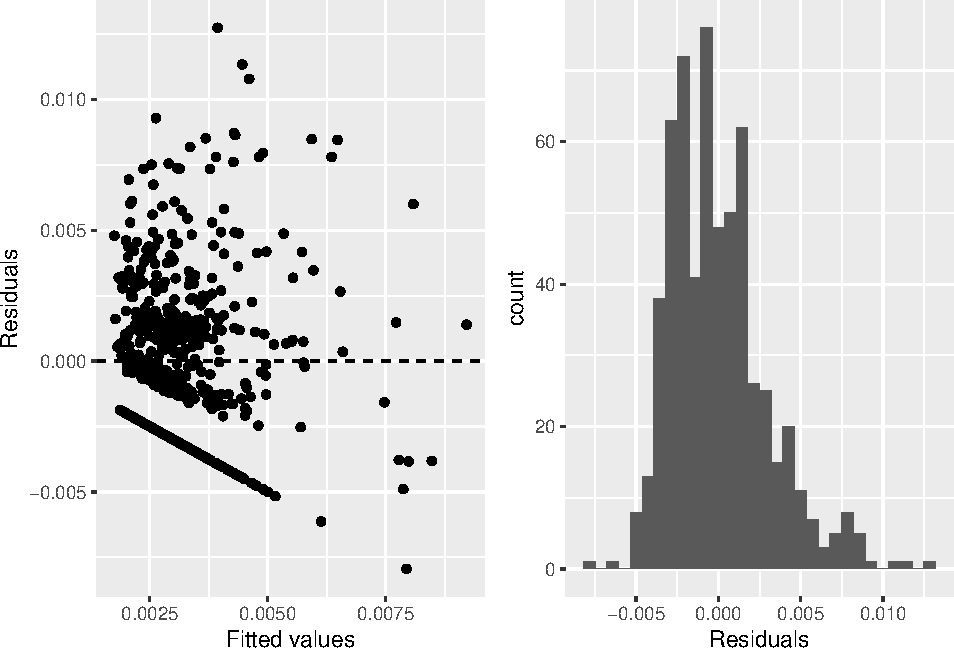
\includegraphics{thesis_files/figure-latex/unnamed-chunk-17-1.pdf}
\caption{\label{fig:unnamed-chunk-17}Observed undervote rate by precinct}
\end{figure}
With an adjusted \(R^2\) value of 0.1402983, the best linear model we found for predicting undervoting\footnote{Here, the percentage of people who listed only 1 or 2 unique candidates out of the percentage of people who listed any number of candidates. This combines both ``undervoting'' as skipping ranking slots and ``duplicated voting'' as ranking the same candidate in multiple slots.} included variables for both race and education. Having more African-Americans and residents over 25 without a high school degree was negatively correlated with undervoting.
\begin{longtable}{lrrrr}
\caption[Linear undervote model]{\label{tab:unnamed-chunk-18}Linear model for undervoting in RCV}\\
\toprule
term & estimate & std.error & statistic & p.value\\
\midrule
Intercept & 0.3007776 & 0.0033039 & 91.0376023 & 0.0000000\\
black & 0.2624983 & 0.0262434 & 10.0024344 & 0.0000000\\
no\_english & -0.0122423 & 0.0200423 & -0.6108239 & 0.5415479\\
\bottomrule
\end{longtable}
\begin{verbatim}
`stat_bin()` using `bins = 30`. Pick better value with `binwidth`.
\end{verbatim}
\begin{figure}
\centering
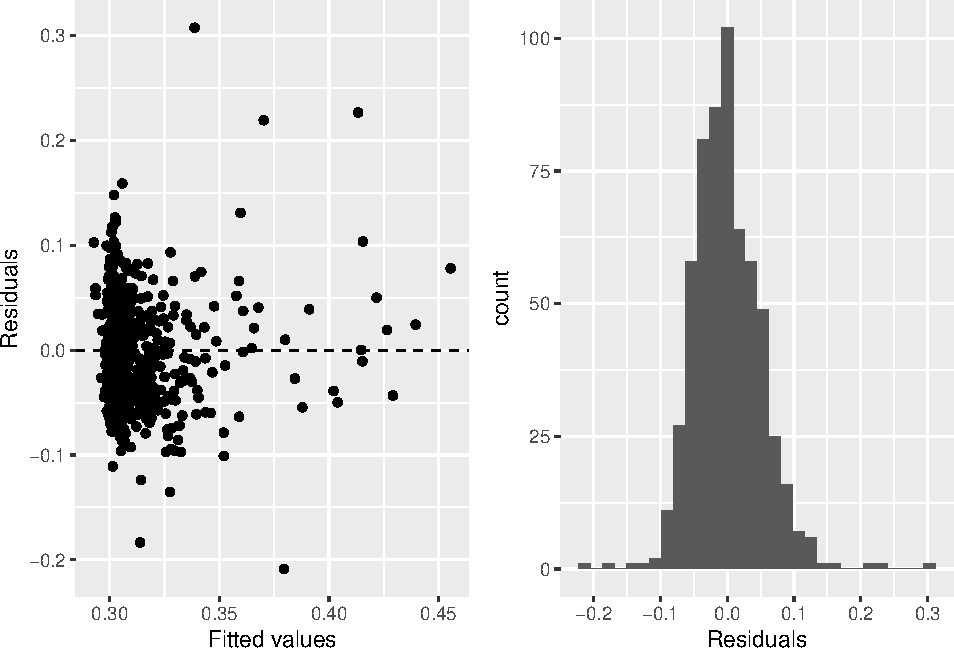
\includegraphics{thesis_files/figure-latex/unnamed-chunk-18-1.pdf}
\caption{\label{fig:unnamed-chunk-18}Linear undervote model validation}
\end{figure}
Honestly I'm really unsure what's going on here. Heavily black precincts are more likely to undervote (lines up with general voting literature), but precincts with less education (less HS grads / less college grads) are less likely to undervote (doesn't line up), and precincts that speak English less well are also less likely to undervote. Just some unexpected and not always significant results.

And these are logistic for over and under - still need to do training/test or cross validation, plus better model selection.
\begin{verbatim}

Call:
glm(formula = cbind(over_count, no_over_count) ~ hispanic + black + 
    no_english, family = binomial, data = sf_precincts)

Deviance Residuals: 
    Min       1Q   Median       3Q      Max  
-2.2423  -1.3196  -0.2044   0.5949   2.4973  

Coefficients:
            Estimate Std. Error z value Pr(>|z|)    
(Intercept) -6.16177    0.06977 -88.318  < 2e-16 ***
hispanic     0.59112    0.29565   1.999   0.0456 *  
black        2.48213    0.36157   6.865 6.66e-12 ***
no_english   1.33077    0.32618   4.080 4.51e-05 ***
---
Signif. codes:  0 '***' 0.001 '**' 0.01 '*' 0.05 '.' 0.1 ' ' 1

(Dispersion parameter for binomial family taken to be 1)

    Null deviance: 750.86  on 601  degrees of freedom
Residual deviance: 688.05  on 598  degrees of freedom
AIC: 1706.8

Number of Fisher Scoring iterations: 5
\end{verbatim}
\begin{verbatim}

Call:
glm(formula = cbind(under_count, no_under_count) ~ +pop_18_24 + 
    pop_25_44 + pop_45_64 + hispanic + white + black + asian + 
    no_hs + college, family = binomial, data = sf_precincts)

Deviance Residuals: 
    Min       1Q   Median       3Q      Max  
-6.5824  -1.1196  -0.0629   1.0966   7.3013  

Coefficients:
            Estimate Std. Error z value Pr(>|z|)    
(Intercept) -1.06027    0.16482  -6.433 1.25e-10 ***
pop_18_24   -1.02998    0.09481 -10.863  < 2e-16 ***
pop_25_44   -1.39112    0.06009 -23.152  < 2e-16 ***
pop_45_64   -1.03105    0.10265 -10.044  < 2e-16 ***
hispanic     0.65881    0.16600   3.969 7.23e-05 ***
white        0.82520    0.16256   5.076 3.85e-07 ***
black        2.13285    0.18690  11.412  < 2e-16 ***
asian        0.66171    0.16103   4.109 3.97e-05 ***
no_hs        0.51201    0.09420   5.435 5.47e-08 ***
college      0.55698    0.06675   8.344  < 2e-16 ***
---
Signif. codes:  0 '***' 0.001 '**' 0.01 '*' 0.05 '.' 0.1 ' ' 1

(Dispersion parameter for binomial family taken to be 1)

    Null deviance: 2764.1  on 601  degrees of freedom
Residual deviance: 1707.0  on 592  degrees of freedom
AIC: 5491.8

Number of Fisher Scoring iterations: 3
\end{verbatim}
Try the glmulti package on the mLab computers, maybe their rJava will work better\ldots?
\url{https://rstudio-pubs-static.s3.amazonaws.com/2897_9220b21cfc0c43a396ff9abf122bb351.html}

\hypertarget{missing-litreview}{%
\chapter{Missing data literature review}\label{missing-litreview}}

\hypertarget{missing-data}{%
\section{Missing data}\label{missing-data}}

Many statistical methods require complete data sets, that is data where every possible observation has a proper value, to work correctly (univariate means, regression, etc.). In many fields of research, however, data collection often results in missing data. Respondents skipping questions (nonresponse), respondents not completing all phases of a multi-stage survey (attrition), government agencies not reporting certain data (redaction), and errors in data collection are all examples of reasons that data can be missing.

Suppose we have a matrix \(X\), with some missing data, which has \(m\) rows and \(n\) columns. Let \(Y = (y_{ij})\) be the complete version of dataset \(X\), that is every missing data point in \(X\) is now observed. Let \(A\) be an \(m \times n\) matrix, where

\[
A = (a_{ij}) \text{, where } a_{ij} =
\begin{cases}
1, \text{ when }x_{ij}\text{ is missing}\\
0, \text{ when }x_{ij}\text{ is not missing}
\end{cases}
\]

Let \(Y_{obs}\) be the observed data in \(Y\), that is the entries in \(Y\) corresponding to the entries in \(A\) that equal 0, and \(Y_{mis}\) be the missing data in \(Y\), that is the entries in \(Y\) corresponding to the entries in \(A\) that equal 1. Let \(\phi\) denote some unknown parameters.

The literature on missing data has identified three distinct subtypes of missing data (Little \& Rubin, 2014).
\begin{itemize}
\item
  Missing completely at random (MCAR). The distribution of missing values does not depend on any data in \(Y\), observed or missing. \[f(A|Y,\phi) = f(A|\phi) \;\forall\; Y,\phi\] An example of this is a survey where the respondent mislabeled a question answer by accident.
\item
  Missing at random (MAR). The distribution of missing values depends on the observed data, but not any missing data. \[f(A|Y,\phi) = f(A|Y_{obs},\phi) \;\forall\; Y_{mis},\phi\] An example of this is an election poll where members of one party are less likely to report their true vote choice than members of another party. The distribution of missing vote choice depends on an observed variable, party identification.
\item
  Non-ignorable (NI), or missing not at random (MNAR). The distribution of missing values depends on the missing values themselves. An example of this is high-income respondents leaving the income field blank in a survey to obscure their true earnings.
\end{itemize}
\hypertarget{methods-of-dealing-with-missing-data}{%
\section{Methods of dealing with missing data}\label{methods-of-dealing-with-missing-data}}

As with any data problem, a common task for a dataset with missing data is to obtain a useful estimator. Let \(\hat{x}\) be an estimator of some population parameter \(x\). Some of the qualities that are good in an estimator are:
\begin{enumerate}
\def\labelenumi{\arabic{enumi}.}
\item
  Lack of bias. \(\hat{x}\) is \emph{unbiased} if \(E(\hat{x}) - x = 0\), that is we expect \(\hat{x}\) to be an accurate guess at \(x\) (Nikulin, n.d.).
\item
  Efficiency. An estimator \(\hat{x}_1\) is more efficient than \(\hat{x}_2\) if the sampling variance of the estimator \(\hat{x}_1\) is less than the variance of the estimator \(\hat{x}_2\), that is we expect \(\hat{x}_1\) to be a more precise guess at \(x\). An unbiased estimator can be called ``efficient'' if its variance is equal to the Cramer-Rao Lower Bound: the inverse of the Fisher Information of the unknown parameter (Fowler, n.d.).
\item
  Provides good estimates of uncertainty. Metrics such as confidence intervals created by the estimator should be accurate (Allison, 2011).
\end{enumerate}
Listed below are some of the methods for dealing with missing data, and the qualities of the estimators they produce.

\hypertarget{listwise-deletion}{%
\subsection{Listwise deletion}\label{listwise-deletion}}

\emph{Listwise deletion} (or \emph{complete-case analysis}) is the most common method of dealing with missing data, as many statistical packages perform listwise deletion on datasets before running most analyses because they need complete data. In listwise deletion, any row with a missing value is fully removed from the dataset. This can lead to biased parameter estimates when the data is not MCAR. Consider the high-income censoring case as above, with average income being the parameter of interest. If high earners are censoring their income and they are dropped from the dataset, our estimate of average income will be negatively biased. Additionally, listwise deletion will reduce the number of overall observations going into any analysis, which reduces the statistical power of methods and increases the size of equivalent confidence intervals (Little \& Rubin, 1987).

In terms of the three goals of an estimator above, listwise deletion performs moderately. It provides good estimates of uncertainty, and can be unbiased under certain conditions (MCAR, and some MAR cases). It is quite inefficient, however, because it tosses away so much available data. Variance increases with a reduction in the number of data points, so you need more data points to obtain an estimator with a desired variance (Allison, 2011).

\hypertarget{maximum-likelihood-estimation}{%
\subsection{Maximum likelihood estimation}\label{maximum-likelihood-estimation}}

\emph{Maximum likelihood estimation} (MLE) methods generally ignore the missing data. The process is similar to any maximum-likelihood-based parameter estimation with full data: all of the available data is used to build a likelihood model for the parameter(s) of interest, and then the likelihood equation is maximized to obtain an estimate. MLE inferences which ignore the missing-data mechanism like this only require MAR to be valid (Little \& Rubin, 1987).

MLE satisfies all of the estimator criteria listed above well, but does have some drawbacks. It takes some computationally intensive software to calculate, and involves fitting some parameters on the data that may or may not apply (Allison, 2011). In our case, because we're dealing with a very complex estimator (election winner as determined by the RCV algorithm) that truly depends on every single data point, any MLE method would be an intensely computational black box that produces a likely uninterpretable result.

\hypertarget{inverse-probability-weighting}{%
\subsection{Inverse probability weighting}\label{inverse-probability-weighting}}

\emph{Inverse probability weighting} (IPW) attempts to correct for the bias of listwise deletion by weighting each observed data point by its probability of being missing. A probability model is specified that determines if a case is complete or not: \(P(\text{complete }|\text{ observed data})\)\footnote{The reader may note that this is similar to the definition of data being missing at random.}. Then a weight is assigned to each case, which is the inverse of its probability of being missing based on the observed data. The desired analysis is then performed with the newly-weighted data (Seaman \& White, 2013).

IPW can outperform listwise deletion in terms of bias, particularly in the MNAR case where the overweighting of similar-to-missing data helps to correct for the bias in listwise deletion. IPW is less efficient than multiple imputation, because it uses only complete cases to build its weights (as opposed to MI, which uses all available data) (Seaman \& White, 2013).

\hypertarget{imputation---single-and-multiple}{%
\subsection{Imputation - single and multiple}\label{imputation---single-and-multiple}}

\emph{Imputation}, unlike the previous three methods, is a way of filling in the missing data points directly\footnote{Rather than going straight to an adjusted conclusion/parameter.}. In \emph{single imputation}, a single value is estimated for each missing cell in the data. Some variants of single imputation are:
\begin{itemize}
\item
  Mean imputation, where the mean of the observed data column is taken. This can lead to biased estimates if the data is not MCAR (the observed data is not representative of the missing data), and also negatively impacts measures of variance.
\item
  Hot deck imputation, where a value from an otherwise similar row in the data is taken. This comes in two subtypes:
  \begin{itemize}
  \tightlist
  \item
    Random hot deck, where a random case is drawn to fill in the missing values.
  \item
    Sequential hot deck, where the most immediately previous matching case is drawn to fill in the missing values.
  \end{itemize}
\item
  Regression imputation, a model-based approach where the missing value is predicted using a regression equation that is trained using the observed data.
\item
  Multinomial imputation, a different model-based approach which is tailored for a categorical response variable.
\item
  Last value imputation, where the missing value is copied from the immediately preceding observed value\footnote{This is similar to sequential hot deck, but last value imputation doesn't have the same concerns about similarity between the cases; it just repeats the immediate last data point measured.}. This is particularly common in time series data, where this is a natural ordering of the observations.
\end{itemize}
\emph{Multiple imputation} (MI) is a method of running single imputation multiple times to create extra variability in your estimates. A dataset is imputed multiple times (with some variability between imputations), then for each new dataset the parameter of interest is calculated. This added variability moderates the appearance of ``certainty'' that comes with single imputation (Little \& Rubin, 1987).

Hot desk imputation is unbiased under MCAR and MAR (Little \& Rubin, 1987). Imputation typically underestimates variance in parameter estimates, because (after a random draw to fill in the data) it uses a deterministic method to calculate the estimate. Multiple imputation can increase this variance through multiple random draws, but still often underestimates variance. Depending on the parameter you're interested in, often five imputations is enough to obtain nearly-efficient estimates with MI (Allison, 2011).

\hypertarget{what-if-everybody-votes-fully}{%
\section{What if everybody votes (fully)?}\label{what-if-everybody-votes-fully}}

The question of ``what if everybody voted'' (or "what if we had 100\% turnout) is one well-studied in literature, and particularly under alternative voting methods including RCV. Consider Table \ref{tab:vote-combo-orig}, which shows the twenty most common combinations of votes in the 2018 SF mayoral election.
\begin{table}[t]

\caption[Original vote counts]{\label{tab:vote-combo-orig}Examination of voter counts}
\centering
\resizebox{\linewidth}{!}{
\begin{tabular}{lllrr}
\toprule
1 & 2 & 3 & Count & Proportion\\
\midrule
LONDON BREED & NA & NA & 20430 & 0.0812656\\
JANE KIM & MARK LENO & AMY FARAH WEISS & 15654 & 0.0622678\\
LONDON BREED & MARK LENO & JANE KIM & 11937 & 0.0474825\\
MARK LENO & JANE KIM & LONDON BREED & 11074 & 0.0440497\\
LONDON BREED & JANE KIM & MARK LENO & 10848 & 0.0431507\\
\addlinespace
JANE KIM & MARK LENO & LONDON BREED & 10484 & 0.0417028\\
MARK LENO & LONDON BREED & JANE KIM & 7705 & 0.0306486\\
JANE KIM & MARK LENO & NA & 7633 & 0.0303622\\
MARK LENO & JANE KIM & NA & 7525 & 0.0299326\\
LONDON BREED & MARK LENO & NA & 6595 & 0.0262333\\
\addlinespace
LONDON BREED & MARK LENO & ANGELA ALIOTO & 6188 & 0.0246144\\
MARK LENO & JANE KIM & ANGELA ALIOTO & 5811 & 0.0231147\\
JANE KIM & LONDON BREED & MARK LENO & 5761 & 0.0229159\\
MARK LENO & NA & NA & 5725 & 0.0227727\\
JANE KIM & MARK LENO & ANGELA ALIOTO & 4649 & 0.0184926\\
\addlinespace
MARK LENO & JANE KIM & AMY FARAH WEISS & 4514 & 0.0179556\\
LONDON BREED & JANE KIM & ANGELA ALIOTO & 4238 & 0.0168577\\
LONDON BREED & ANGELA ALIOTO & MARK LENO & 4231 & 0.0168299\\
LONDON BREED & ANGELA ALIOTO & NA & 3548 & 0.0141131\\
ANGELA ALIOTO & NA & NA & 3524 & 0.0140176\\
\bottomrule
\end{tabular}}
\end{table}
The most common vote choice was London Breed and nobody else\footnote{Breed herself may have increased the rate of appearance of this combination. When asked at a candidate forum who her second and third choices for mayor would be, she replied ``My No.~2 choice is London Breed, and my No.~3 choice is London Breed'' (Berman, 2018). An interesting study would be to see if ``London Breed'' repeated 3 times shows up more often than we would expect it to, given how often other candidates appear 3 times.}, which shows the potential for many more people to fill in 2nd and 3rd vote choices\footnote{This data has been cleaned to consolidate repeated vote choices, so there is no difference between listing only ``London Breed'' as first or listing her in all three slots.}. While this (and most other undervotes in the first few rows here) would not have changed the election result because of how they voted for final candidates, consider row 20: people who only voted for Angela Alioto, the eventual fourth-place finisher. There were 3,524 people who voted for Alioto alone, which is larger than the final margin of 2,268 between London Breed and Mark Leno. The presence of undervotes like this has the potential to change the results of an election.

Citrin, Schickler, \& Sides (2003) use auxiliary data to simulate vote choice of non-voters in US Senate elections. They raise an interesting consideration: while the overarching metric of electoral change is an election flipping, the numerical ``amount'' of change in an election may be large but not enough to overcome a yet larger margin of victory. For example, if full voter turnout improved Democratic vote shares by 5\% across the country, this would only flip the seats where a) a Democrat lost, and b) the margin of victory for the other candidate was small enough that a 5\% vote share would overturn it. We should thus consider alternate methods of assessing the impact of no undervotes or overvotes, aside from looking at who wins the election.

Liu (2014) investigates imputation methods for vote choice in a Taiwanese election (conducted with plurality). They find that ``the extent to which MI corrects the distribution {[}of vote share{]} is very limited, although the direction of adjustment is correct''. Bernhagen \& Marsh (2010) use multiple imputation to simulate choices in place of undervotes in an Irish general election (conducted with RCV). They find that the techniques applied were normally ``not large enough to affect the counterfactual estimation of election results under universal turnout''. These studies seem to indicate that MI may not be a technique which will change our election results enough to be noticeable. Further work could be done into how well MI mirrors the correct amount of variance under different conditions (MCAR, MAR, etc.).

In a FairVote report, S. Hill \& Hernandez (2018) find a similar result in the 2018 San Francisco mayoral election: the exhausted ballots in this election did not have the potential to swing the election away from Breed. They also find that the majority of exhausted ballots were ``voluntarily exhausted'' meaning that the voter undervoted, rather then being exhausted because they ran out of available slots to list. Additionally, the involuntarily exhausted ballots were likely to pull for London Breed over Leno. In addition to the small impacts of MI mentioned above, this study indicates that the positioning of the undervotes themselves in this specific election may be a factor that contributes to a lack of change in our results. Taking this into concern in combination with the MI result, we may expect to not see much variance among methods.

\hypertarget{peculiarities-with-this-study}{%
\section{Peculiarities with this study}\label{peculiarities-with-this-study}}

\hypertarget{violated-assumptions}{%
\subsection{Violated assumptions}\label{violated-assumptions}}

\protect\hyperlink{missing-data}{Earlier} we made the implicit assumption that every ``missing'' data point (unobserved value) has some true value. In the case of ranked-choice voting, this is not necessarily true. It is a fully rational choice for a voter to only list one candidate when offered three options, if they truly only have one preference. While this would seem to make this study just an exercise in missing data methods, this is no more the case here than in other studies of imputing vote choice.

Kroh (2006) has a good discussion of methods for working with imputations when ``Don't know'' is a valid response, or there are valid reasons for the inapplicability of a survey question. While Kroh's study does not apply to our particular research question and data, it provides a nuanced take on the assumptions inherent in missing data imputation.

\hypertarget{monotonicity}{%
\subsection{Monotonicity}\label{monotonicity}}

In particular, our data is \emph{monotone} missing data - that is, for a certain order of our variables \((Y_i)\), an observation having a missing value in column \(Y_j\) implies that it has a missing value in all columns \(Y_J\) where \(J > j\) (Little \& Rubin, 2014). In our case, what this looks like is that you cannot have a third choice for mayor without having a second choice present\footnote{Or rather, we have enforced this condition on our data. We treat the presence of a third choice and the absence of a second choice in a given voter's ballot as an error, and re-align our data so that the unique choices provided by each voter are filled in ``minimally'' to satisfy this monotone condition. We consider such an enforcement to be reasonable, given our access to voter's true preferences being limited to their reporting as such on the ballot.}. There are additional methods that can be used with monotone data, on which we do not go into greater detail here. These are described at more length in Rubin (1974).

\hypertarget{not-all-undervotes-are-created-equal}{%
\subsection{Not all undervotes are created equal}\label{not-all-undervotes-are-created-equal}}

In the imputation process, we fill in all undervotes\footnote{And weight them, in quantitative analyses.} as if they are treated equally. This is not the case, however, as the undervote of somebody who listed Mark Leno first is inherently not the same as that of somebody who listed Jane Kim first, because she was eliminated in the tabulation process. We must treat these equally, however, because under a given imputation we do not know which candidates will eventually be eliminated. This also maintains the spirit of our research question, ``what if there were no undervotes''.

\hypertarget{turnout}{%
\subsection{100\% turnout}\label{turnout}}

Due to data limitations, in this study we did not truly ask ``what if everybody voted'', but instead ``what if there were no overvotes or undervotes''. This is a different question, both conceptually and in practice: the latter question does not involve inferring the preferences of total non-voters, for example. This is an intriguing question for further study, but in this particular research we were examining the phenomena of overvoting and undervoting, rather than nonvoting. Some of the literature above is particular to the idea of 100\% turnout, but still has important insight into our research question.

\hypertarget{missing-methods}{%
\chapter{Missing data methods}\label{missing-methods}}

\hypertarget{imp-methods}{%
\section{Imputation}\label{imp-methods}}

In dealing with our missing data, we chose here to use multiple imputation for a handful of reasons. First, it had the best conceptal analog to ``what if there were no overvotes or undervotes'', and is thus an appropriate method for measuring the effect of said ballot phenomena. Second, it does not have the same distributional assumptions that come with methods like maximum likelihood estimation. There were six methods of dealing with the missing data that we used:
\begin{itemize}
\item
  Original cases (or, not dealing with it at all). This original election data is a baseline case to compare all methods applied to.
\item
  Listwise deletion. This is one form of analog to ``what if there were no overvotes or undervotes'', but instead of using all of the available information on voters it removes incomplete information and leaves us with a less accurate measure. This does, however, give us a ``full vote choice distribution'' from the original ballots that we can use to compare to other methods.
  \begin{table}[t]

    \caption[Listwise vote counts]{\label{tab:unnamed-chunk-20}Examination of full voter counts}
    \centering
    \resizebox{\linewidth}{!}{
    \begin{tabular}{lllrr}
    \toprule
    1 & 2 & 3 & Count & Proportion\\
    \midrule
    JANE KIM & MARK LENO & AMY FARAH WEISS & 15654 & 0.0903336\\
    LONDON BREED & MARK LENO & JANE KIM & 11937 & 0.0688841\\
    MARK LENO & JANE KIM & LONDON BREED & 11074 & 0.0639041\\
    LONDON BREED & JANE KIM & MARK LENO & 10848 & 0.0625999\\
    JANE KIM & MARK LENO & LONDON BREED & 10484 & 0.0604994\\
    \addlinespace
    MARK LENO & LONDON BREED & JANE KIM & 7705 & 0.0444628\\
    LONDON BREED & MARK LENO & ANGELA ALIOTO & 6188 & 0.0357087\\
    MARK LENO & JANE KIM & ANGELA ALIOTO & 5811 & 0.0335332\\
    JANE KIM & LONDON BREED & MARK LENO & 5761 & 0.0332447\\
    JANE KIM & MARK LENO & ANGELA ALIOTO & 4649 & 0.0268277\\
    \bottomrule
    \end{tabular}}
    \end{table}
  This full vote choice distribution lets us compare these methods at a more granular level than the simple parameter of ``who won''. For example, we can see what proportion of voters under our multinomial method below voted for the \texttt{Kim\ -\ Leno\ -\ Weiss} combination, compared to the 9.03\% of full voters that had this combination in the original ballot.
\item
  Random hot deck imputation (RHD) based on nothing: that is, each voter is assigned a truly random candidate (pulled from the existing distribution of that ranking slot) that is unique from their earlier vote choices. This ignores some of the conditional distribution information available in the data. For example, given the cross-endorsement between Jane Kim and Mark Leno, we might expect their voters to be more likely to support the other candidate as their second choice than an average voter. Randomly pulling a second choice to impute for a Kim voter would then underestimate the chance that Kim would have been chosen.
\item
  RHD based on vote choice alone. Missing data points are matched to potential donors by their corresponding 1st vote choice when imputing the 2nd vote choice, and by their first two vote choices when imputing the 3rd vote choice. This solves some of the conditional information problems presented by the fully random imputation.
\item
  RHD based on vote choice and precinct. This is similar to the imputation vote choice alone, but now donors also must be from the same precinct as the recipient. This method controls for which precinct the voter is from, which attempts to get at differences between precincts in candidate support.
\item
  Multinomial logistic regression based on vote choice and demographic data. The demographic information given to each voter was the rates of demographic groups in their precinct\footnote{This leaves us somewhat open to the genetic fallacy of assuming that every person in a precinct is identical to the precinct as a whole. However, since we are not interpreting the coefficients of this model, this precinct demographic information can just be treated as more information to make an accurate predictive model. It is a way of quantifying how similar different precincts are to each other, rather than simply treating each one as a wholly independent entity.}, as described in \protect\hyperlink{demo-methods}{Chapter 2}. This is similar to a multinomial regression based on vote choice and precinct alone, but also includes more information about certain precincts being more demographically similar than others.
\end{itemize}
\hypertarget{issues}{%
\subsection{Issues}\label{issues}}

\hypertarget{rubins-rules}{%
\subsubsection{Underestimate of variance}\label{rubins-rules}}

As expressed in the \protect\hyperlink{missing-litreview}{previous chapter}, single imputations underestimate variance because they place an unwarranted certainty upon the newly imputed data, which is then fed into a deterministic process to calculate an estimator. This is overcome through the use of multiple imputation.

There are a set of methods to calculate the mean and variance of estimators from multiple imputation, known as ``Rubin's Rules'' (Heymans \& Eekhout, 2009). For a set of estimates \(\{\hat{\theta}_i\}\) of a parameter \(\theta\) and \(m\) the number of imputations, the pooled mean can be calculated
\[
\bar{\theta} = \frac{1}{m} \sum_{i=1}^m \hat{\theta}_i,
\]
that is the mean of the estimates.

For variance, we must consider two quantities. Within each imputation, any estimate will have a standard error \(SE_i\)\footnote{If our estimate is a mean, this is the standard deviation of the vector divided by the square root of the sample size. If the estimate is a proportion \(\hat{p}\), the standard error is \(\sqrt{\hat{p} (1 - \hat{p}) / n}\).}. We can then calculate the overall variance \emph{within} imputations,
\[
V_W = \frac{1}{m} \sum_{i=1}^m SE_i^2,
\]
the average squared standard error within an imputation. There is also variance \emph{between} each dataset, which comes from uncertainty about what the true values are that we are attempting to impute. This is expressed as
\[
V_B = \sqrt{\frac{\sum_{i=1}^m (\theta_i - \bar{\theta})^2}{m-1}},
\]
that is the sample variance of the estimators. Then, the \emph{total} variance of our estimate is
\[
V_T = V_W + V_B + \frac{V_B}{m},
\]
a combination of these two facets of variance. This is the way in which multiple imputation adjusts for the decreased variance that comes with single imputation.

While our RCV algorithm does not produce typical sample parameter estimates, these rules are still useful for obtaining an accurate sense of variability in our quantitative estimates.

\hypertarget{imputation-on-an-imputation}{%
\subsubsection{Imputation on an imputation}\label{imputation-on-an-imputation}}

Since we impute the 3rd choice based on the first and second choices, this means we're imputing some rows based on the imputed (unobserved) 2nd choice. This can lead to further issues of certainty, because the further imputations treat the imputed 2nd choice as known. We also believe this is overcome through the use of multiple imputations.

\hypertarget{incomplete-hot-deck-matching}{%
\subsubsection{Incomplete hot deck matching}\label{incomplete-hot-deck-matching}}

Some combinations of vote choices (typically including unpopular candidates), or precinct and vote choices, are unique or not present in the data. This means that the hot deck method cannot match any donor to impute a value. When this is the case, we then fill in with the next-best method, that is: if there is no combination of 1st and 2nd that matches the case we need to impute 3rd for, we fall back to just matching 1st and imputing the value. Table \ref{tab:no-rhd-match} is an illustration of how often this phenomenon happens.
\begin{longtable}{lr}
\caption[Imputation mismatches - 3rd choice]{\label{tab:no-rhd-match}Proportion of unfilled 3rd vote choices through imputation steps}\\
\toprule
Imputation step & Proportion\\
\midrule
Original & 0.3106906\\
1st, 2nd choice \& precinct & 0.0057996\\
1st, 2nd choice & 0.0000040\\
1st choice & 0.0000000\\
\bottomrule
\end{longtable}
Even in the worst case scenario out of all the imputations (3rd vote choice, imputed on 1st choice, 2nd choice, and precinct), only 0.580\% of 3rd vote choices are missing. Of the choices that were missing originally, even this method is able to match 98.1\% of them. Since this is a small problem, we feel it does not negatively impact our results.

\hypertarget{choice-of-which-imputations-to-perform}{%
\subsubsection{Choice of which imputations to perform}\label{choice-of-which-imputations-to-perform}}

There are any number of alternative imputation methods we could have used to get simulated elections. The ones here were chosen for a mix of applicability (not all methods apply to cetegorical data as well as numerical data), feasibility, and our subjective assessment of what would make an interesting comparison\footnote{E.g., the missing data methods progress from least information used (listwise deletion) to most information used (all available vote choices and precinct demographic information).}.

For all of these methods, we had to ensure that no duplicate votes were created in the process\footnote{As this would represent an ``undervote'', not using as many unique candidates as allowed.}. For example, a multinomial model considering demographic information alone (no vote choices) was considered, but did not work because it created duplicated votes for a number of the voters.

\hypertarget{data-preparation}{%
\section{Data preparation}\label{data-preparation}}

The election data was transformed first, to remove any duplicated votes (e.g., a row listing London Breed three times was reduced to its functional equivalent: listing London Breed once) and ``left-align'' all ballots so that ballots with one missing value always had it in slot 3, and ballots with two missing values always had them in slots 2 and 3.

The demographic data used is the same that was used to answer the previous research question: precinct-level demographic rates, obtained through areal interpolation, and joined to each voter by their precinct. This is the most granular method we have to establish demographics for each voter, because the only identifying information we have about any given voter is their precinct. As such, the multinomial model used is not considering a voter's personal demographics, but rather the demographics of their precinct at large. As mentioned earlier, this gives us a way to quantify certain precincts as being more or less ``distant'' demographically to each other, as opposed to treating them all fully independently.

\hypertarget{metrics-for-comparing-methods}{%
\section{Metrics for comparing methods}\label{metrics-for-comparing-methods}}

At the end of the day, the ultimate metric of any election-related experiment like this is the winner of the election. While we are foremostly concerned with this, other metrics should not be ignored for consideration as well. We also examine:
\begin{itemize}
\item
  London Breed's\footnote{Breed was the winner of the real-life election.} vote share in the final round of counting. This metric gives us a quantitative assessment of how close an election was to changing its eventual winner. Here we ignore exhausted ballots and just consider the binary comparison between the final two candidates.
\item
  Intermediate switches in rankings. The smaller absolute margins between candidates in earlier rounds of counting provide a potentially easier opportunity to change the ultimate result (who is elected). These have a cascading effect on later rounds of the election, so even a seemingly insignificant swap in an earlier round of the tabulation can impact the eventual winner.
\item
  Changes in proportions of vote combinations. This makes use of the calculated proportions of each combination of vote choices from the \protect\hyperlink{imp-methods}{listwise deletion} mentioned earlier. This is an attempt at a quantitative assessment of these intermediate ranking swaps, to see how big the impact of the imputation was. If a method has a strangely high or low proportion of a certain vote choice combination compared to the original data (here equivalent to the listwise deletion), then that method may have had some serious impact on the election results.
\item
  Number of exhausted voters by the final round. This is secondary in terms of electoral impact, but does illustrate the impact of undervotes on representation. One of the complaints against RCV is that it has large numbers of exhausted ballots by the final round of the election (depending on how many candidates run and how many candidates voters are allowed to rank). By removing the undervotes and overvotes, we can see how much of the ballot exhaustion phenomenon is attributable to the limit on voter rankings.
\end{itemize}
\hypertarget{missing-results}{%
\chapter{Data imputation results}\label{missing-results}}
\begin{table}[t]

\caption[Election results - original]{\label{tab:orig-results}Original election results}
\centering
\resizebox{\linewidth}{!}{
\begin{tabular}{lrrrrrrrr}
\toprule
Candidate & Round 1 & Round 2 & Round 3 & Round 4 & Round 5 & Round 6 & Round 7 & Round 8\\
\midrule
BREED & 91918 & 91921 & 92039 & 92233 & 93363 & 96028 & 101335 & 113247\\
LENO & 61276 & 61276 & 61392 & 61734 & 62675 & 63837 & 67902 & 110979\\
KIM & 60644 & 60644 & 60735 & 61320 & 61727 & 63059 & 65549 & NA\\
ALIOTO & 17447 & 17447 & 17628 & 17810 & 19463 & 21609 & NA & NA\\
ZHOU & 9521 & 9521 & 9631 & 9758 & 10526 & NA & NA & NA\\
\addlinespace
GREENBERG & 7016 & 7016 & 7093 & 7189 & NA & NA & NA & NA\\
WEISS & 1661 & 1661 & 1720 & NA & NA & NA & NA & NA\\
BRAVO & 890 & 890 & NA & NA & NA & NA & NA & NA\\
ROGERS & 3 & NA & NA & NA & NA & NA & NA & NA\\
NA & 3640 & 3640 & 3778 & 3972 & 6262 & 9483 & 19230 & 29790\\
\bottomrule
\end{tabular}}
\end{table}
For context, Table \ref{tab:orig-results} gives the original election tabulation\footnote{This differs slightly from the official results in (``Ranked Choice Voting Results Table,'' 2018); specifically, our vote counts are consistently an undercount of the official results. We believe this differece is due to the omission of some ballots from the published data, particularly ballots with a scanning error that have to be hand-counted.}.

\hypertarget{final-winner}{%
\section{Final winner}\label{final-winner}}

We see in Table \ref{tab:method-results} that London Breed wins consistently in all methods except the fully random hot deck imputation, in which Mark Leno was consistently elected. As this is the least ``realistic'' of any of the methods (since it uses the least available information to predict vote choice), we can consider it a less accurate measure of potential change. It does potentially indicate that Leno had more overall support than Breed (in terms of being listed anywhere on the ballot), just positioned in the wrong place for it to push him to victory. Perhaps under a different voting system such as Borda count, which awards points to candidates based on any ranking they appeared in, Leno would have won.
\begin{table}[t]

\caption[Winner by method]{\label{tab:method-results}Election results count by method}
\centering
\begin{tabular}{llr}
\toprule
Method & Candidate & First place finishes\\
\midrule
Original ballot & BREED & 1\\
Listwise deletion & BREED & 1\\
Hot deck - random & LENO & 360\\
Hot deck - vote choice & BREED & 360\\
Hot deck - vote choice, precinct & BREED & 360\\
\addlinespace
Multinomial logistic regression & BREED & 360\\
\bottomrule
\end{tabular}
\end{table}
\hypertarget{london-breeds-final-vote-share}{%
\section{London Breed's final vote share}\label{london-breeds-final-vote-share}}
\begin{figure}
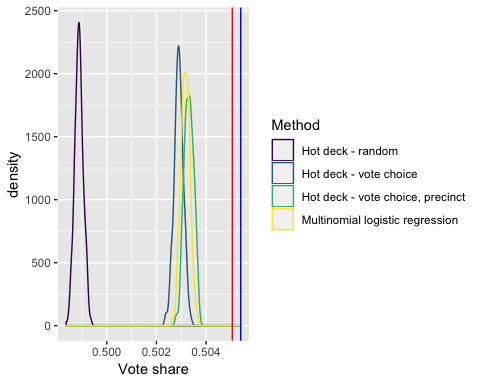
\includegraphics[width=6in]{thesis_files/figure-latex/unadj-breed-1} \caption{London Breed's simulated vote share - unadjusted variances}\label{fig:unadj-breed}
\end{figure}
Figure \ref{fig:unadj-breed} is a density plot representing London Breed's estimated final vote share across the four imputation methods. The red vertical line is the original vote share, and the blue line is her share under listwise deletion. The imputation methods that use more information\footnote{Everything except the fully random hot deck.} indicate that Breed would likely still win if there were no undervotes or overvotes, but her margin of victory would be smaller than it was in the actual election. This could potentially offer some support for the claim that ``the extent to which MI corrects the distribution {[}of vote share{]} is very limited, although the direction of adjustment is correct'' (Liu, 2014).

For each imputation method, we have calculated the estimated mean and variance (using \protect\hyperlink{rubins-rules}{Rubin's rules}) of London Breed's calculated final vote share\footnote{Here a more typically specified question might be: out of all the voters who listed either London Breed or the other calculated finisher in the top two spots (Mark Leno or Jane Kim), what proportion preferred Breed to the other candidate?}. One of the assumptions for using these rules is that the parameter estimates be normally distributed, which they appear to be from Figure \ref{fig:unadj-breed}. We assess that as follows:
\begin{figure}
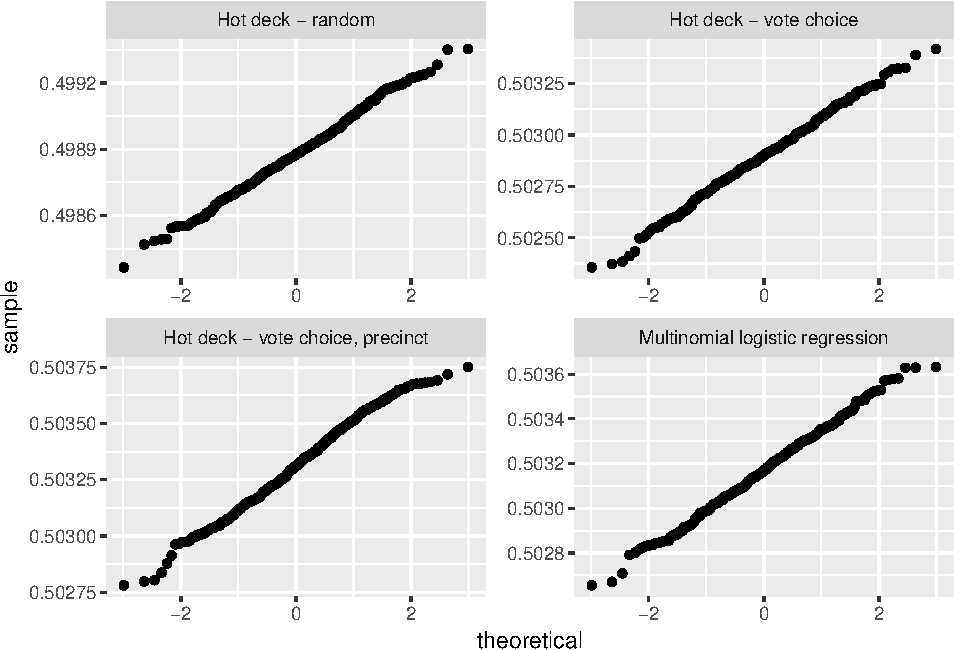
\includegraphics[width=6in]{thesis_files/figure-latex/unnamed-chunk-22-1} \caption{Normality check, Q-Q plot of Breed's vote share}\label{fig:unnamed-chunk-22}
\end{figure}
The Q-Q plots all follow a sufficiently linear path to assume normality in the data, so we meet the assumption to use Rubin's rules here.
\begin{table}[t]

\caption{\label{tab:adj-breed-tab}London Breed's simulated vote share - adjusted variances}
\centering
\begin{tabular}{lrrrr}
\toprule
Method & $\hat{p}$ & $V_W$ & $V_B$ & $V_T$\\
\midrule
Original ballot & 0.5050574 & 0.2499744 & 0 & 0.0000000\\
Listwise deletion & 0.5053969 & 0.2499709 & 0 & 0.0000000\\
Hot deck - random & 0.4988793 & 0.0006944 & 0 & 0.0006945\\
Hot deck - vote choice & 0.5028990 & 0.0006944 & 0 & 0.0006945\\
Hot deck - vote choice, precinct & 0.5033102 & 0.0006944 & 0 & 0.0006945\\
\addlinespace
Multinomial logistic regression & 0.5031699 & 0.0006944 & 0 & 0.0006944\\
\bottomrule
\end{tabular}
\end{table}
When we apply Rubin's rules to correct our underestimate of variance, the situation changes wildly\footnote{Here the black and brown lines are the vote share for the original and listwise methods (respectively), which overlap at this scale.}. Looking at Figure \ref{fig:adj-breed-plot}, the overlap between the various methods is much more palpable. Breaking this down in Table \ref{tab:adj-breed-tab}, it is clear that the majority of the variance in these estimated distributions comes from the variance \emph{within} each imputation, as opposed to the variance \emph{between} the imputations\footnote{Given the high number of imputations we made (360), as opposed to the 5 that typically suffice for MI, this makes some sense.}. This explains why the unadjusted variance in Figure \ref{fig:unadj-breed} is so small: because it only considers the variance between each imputation.
\begin{figure}
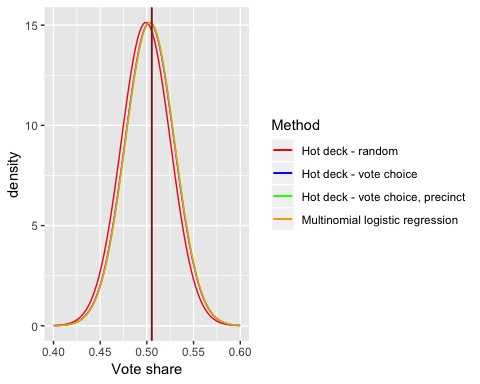
\includegraphics[width=6in]{thesis_files/figure-latex/adj-breed-plot-1} \caption{London Breed's simulated vote share - adjusted variances}\label{fig:adj-breed-plot}
\end{figure}
\hypertarget{intermediate-switches-in-rankings}{%
\section{Intermediate switches in rankings}\label{intermediate-switches-in-rankings}}
\begin{table}[t]

\caption[Simulated candidate rankings]{\label{tab:ranking-count}Candidate ranking for each imputation method}
\centering
\resizebox{\linewidth}{!}{
\begin{tabular}{lrlllllllll}
\toprule
Method & Count & Rank 1 & Rank 2 & Rank 3 & Rank 4 & Rank 5 & Rank 6 & Rank 7 & Rank 8 & Rank 9\\
\midrule
Original ballot & 1 & BREED & LENO & KIM & ALIOTO & ZHOU & GREENBERG & WEISS & BRAVO & ROGERS\\
Listwise deletion & 1 & BREED & KIM & LENO & ALIOTO & ZHOU & GREENBERG & WEISS & BRAVO & ROGERS\\
Hot deck - random & 360 & LENO & BREED & KIM & ALIOTO & ZHOU & GREENBERG & WEISS & BRAVO & ROGERS\\
Hot deck - vote choice & 360 & BREED & LENO & KIM & ALIOTO & ZHOU & GREENBERG & WEISS & BRAVO & ROGERS\\
Hot deck - vote choice, precinct & 360 & BREED & LENO & KIM & ALIOTO & ZHOU & GREENBERG & WEISS & BRAVO & ROGERS\\
\addlinespace
Multinomial logistic regression & 360 & BREED & LENO & KIM & ALIOTO & ZHOU & GREENBERG & WEISS & BRAVO & ROGERS\\
\bottomrule
\end{tabular}}
\end{table}
Table \ref{tab:ranking-count} shows that each of the methods has the exact same candidate across all of the simulations run\footnote{There were 360 simulations run for the imputation methods, and the two deterministic methods (original ballot data and listwise deletion) were each calculated once.}. Under listwise deletion, we see that Jane Kim edged out Mark Leno as runner-up, but still failed to defeat Breed. Under the fully random imputation, Leno took first place from Breed, but the remaining candidates are still arranged as they were in the original election.

We see no variability among these candidate rankings within each imputation method. While there were small changes in vote counts within methods between each simulation (see \protect\hyperlink{vote-combo-results}{Section 6.4}), this was not enough to change the eventual ordering of the candidates within any imputation method. However, between methods we do see some slight variability. As mentioned above, listwise deletion and fully random imputation are the least informed of the methods, so we consider their candidate rearrangements to be less accurate than the consistency in the more-informed methods.

\hypertarget{vote-combo-results}{%
\section{Distribution of vote combinations}\label{vote-combo-results}}

For each imputation method, we can compare the rate of appearance of a single vote combination to the baseline generated from the listwise deletion.
\begin{figure}
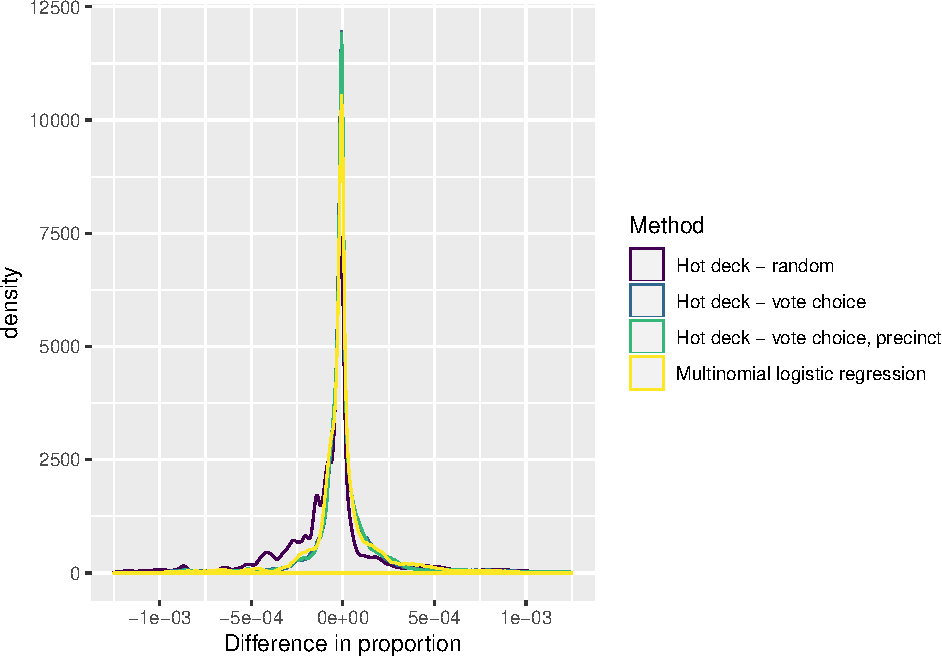
\includegraphics[width=6in]{thesis_files/figure-latex/vote-combos-1} \caption{Difference in vote combination rates}\label{fig:vote-combos}
\end{figure}
Figure \ref{fig:vote-combos} is a density plot displaying the difference between the rate of a given vote combination under listwise deletion to its rate in each of the imputed methods. Overall, these changes in proportion from the original data are very small, which would seem to indicate that the imputation methods aren't actually changing the distribution of the data as a whole. This makes some sense, and lines up with our observations so far that the imputation methods (particularly the more informed ones) don't impact the electoral results very much. Additionally, this highlights that these imputation methods suffer from the same ``sampling issue'' that techniques like bootstrapping have. Since we're trying to extrapolate from our data set, any inferences that we draw will be inherently centered around that observed data in some way.

\hypertarget{exhausted-voters-by-the-final-round}{%
\section{Exhausted voters by the final round}\label{exhausted-voters-by-the-final-round}}
\begin{figure}
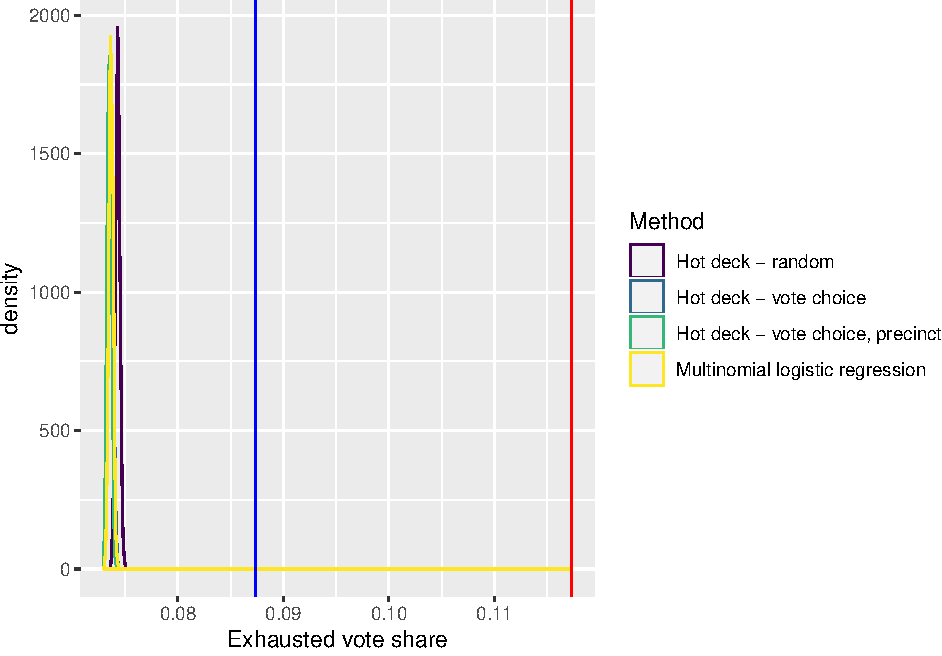
\includegraphics[width=6in]{thesis_files/figure-latex/unadj-exhausted-1} \caption{Simulated exhausted vote share - unadjusted variances}\label{fig:unadj-exhausted}
\end{figure}
Figure \ref{fig:unadj-exhausted} is a density plot of the proportion of exhausted votes for each imputation method. The red line is exhausted votes in the original data, and the blue line is exhausted votes after listwise deletion. We see that the unadjusted variance for each method is small, compared to the overall decrease in exhausted votes from the original ballot data. The exhausted vote share in our imputed datasets is about 62.9\% of the exhausted vote share in the original election. This indicates that about 0.4 of the exhausted data issue is ``voluntary'', where voters are not ranking as many candidates as they are given the option to.

We again apply Rubin's rules to calculate the estimated mean and variance of the final exhausted vote share\footnote{Here a specified question might be: out of all the voters, how many did not support either of the top two finishers?}. Checking the normal assumption:
\begin{figure}
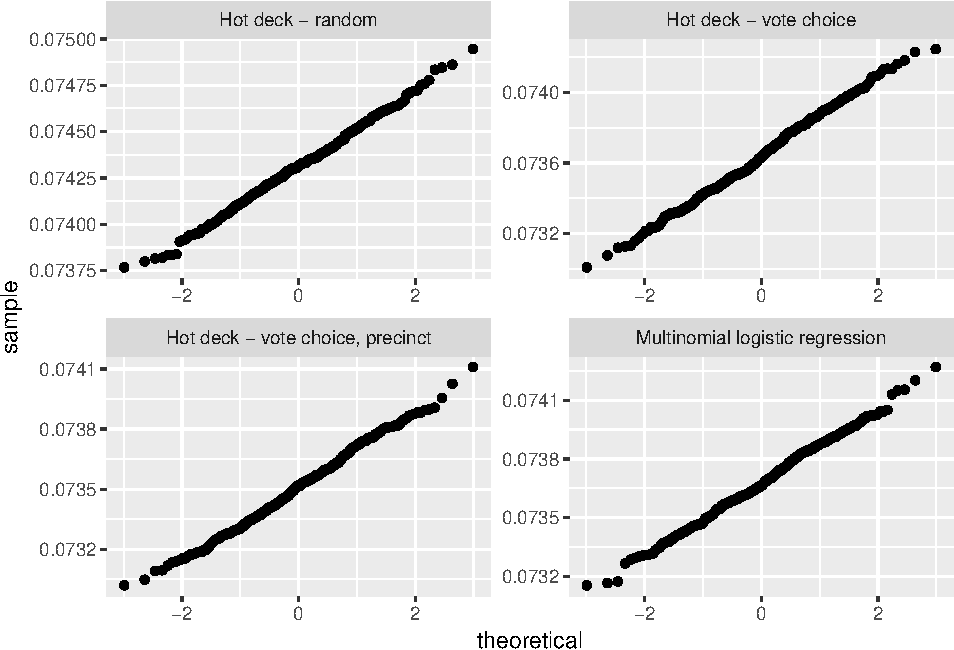
\includegraphics[width=6in]{thesis_files/figure-latex/unnamed-chunk-23-1} \caption{Normality check, Q-Q plot of exhausted vote share}\label{fig:unnamed-chunk-23}
\end{figure}
Since the Q-Q plots are sufficiently linear, we can assume that our parameter estimates for share of votes exhausted by the final round are normally distributed and proceed with Rubin's rules.
\begin{longtable}{lrrrr}
\caption[Simulated exhausted votes]{\label{tab:adj-exhausted-tab}Exhausted votes for each imputation method}\\
\toprule
Method & $\hat{p}$ & $V_W$ & $V_B$ & $V_T$\\
\midrule
Original ballot & 0.1172761 & 0.1035224 & 0e+00 & 0.0000000\\
Listwise deletion & 0.0873906 & 0.0797535 & 0e+00 & 0.0000000\\
Hot deck - random & 0.0743117 & 0.0001911 & 0e+00 & 0.0001911\\
Hot deck - vote choice & 0.0736412 & 0.0001895 & 1e-07 & 0.0001895\\
Hot deck - vote choice, precinct & 0.0735096 & 0.0001892 & 0e+00 & 0.0001892\\
\addlinespace
Multinomial logistic regression & 0.0736782 & 0.0001896 & 0e+00 & 0.0001896\\
\bottomrule
\end{longtable}
When we apply Rubin's rules to correct our underestimate of variance, the situation changes wildly\footnote{Here the black and brown lines are the exhausted vote share for the original and listwise methods (respectively).}. Looking at Figure \ref{fig:adj-exhausted-plot}, the overlap between the various methods is much more palpable. Similar to Breed's vote share, Table \ref{tab:adj-exhausted-tab} shows that the majority of the variance in these estimated distributions of exhausted vote share comes from the variance \emph{within} each imputation, as opposed to the variance \emph{between} the imputations. In this case, however, the improvement in exhausted vote share compared to the original data is so high that there is a much clearer impact from the imputation.
\begin{figure}
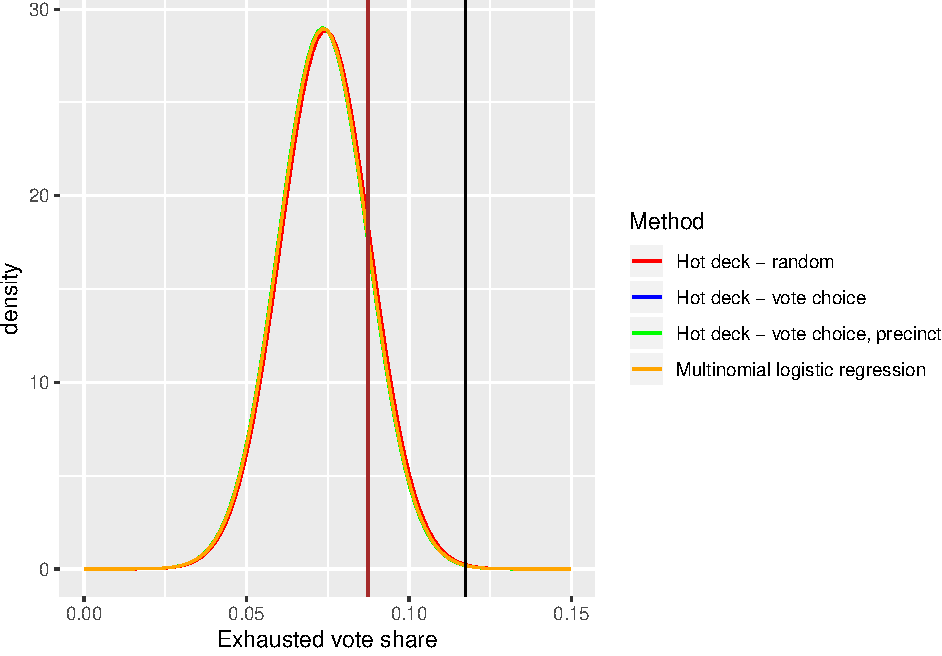
\includegraphics[width=1\linewidth]{thesis_files/figure-latex/adj-exhausted-plot-1} \caption{Simulated exhausted vote share - adjusted variances}\label{fig:adj-exhausted-plot}
\end{figure}
\hypertarget{conclusion}{%
\chapter*{Conclusion}\label{conclusion}}
\addcontentsline{toc}{chapter}{Conclusion}

\hypertarget{summary-of-results}{%
\section{Summary of results}\label{summary-of-results}}

\hypertarget{part-1-1}{%
\subsection{Part 1}\label{part-1-1}}

The results from Part 1 didn't tell us a whole ton that's new. The demographic study seemed to reflect the same trends that we see in voting more generally, which is important but doesn't give any new input on how to better target voter education efforts.

\hypertarget{part-2-1}{%
\subsection{Part 2}\label{part-2-1}}

Given the disparity in undervote levels between different precincts (and the impact of demographic factors on these undervote levels), I expected one of the models with precinct or demographic to have more of an effect (despite the research presented in \protect\hyperlink{missing-litreview}{Chapter 4}. We thought that if the precincts had different local preferences, then the now-higher weighting of underrepresented precincts might change the results. One possible explanation is that this disparate precinct weighting did happen and it cancelled out between different precincts on the whole. Fairvote has produced some analysis that seems to indicate regional distinctions among candidates, which could support the claim about different local preferences (``SF Mayor's Race,'' n.d.-a; ``SF Mayor's Race,'' n.d.-b; ``SF Mayor's Race,'' n.d.-c; ``SF Mayor's Race,'' n.d.-d). Another answer is that MI itself does not produce enough variance to meaningfully affect these election results, given the large number of data points and the inherent closed loop in using the observed data to modify itself. Additionally, as indicated in S. Hill \& Hernandez (2018), the positioning of the undervotes themselves in this election may have had an effect on how much change the process of imputing their values could induce.

\hypertarget{future-research-ideas}{%
\section{Future research ideas}\label{future-research-ideas}}

The most apparent next course of action in this resarch is to extend to more elections and jurisdictions that use RCV. This was not accomplished in this thesis due to issues with obtaining and merging the correct geographic boundaries to obtain precinct demographic information for more than one election cycle or more than one city. The advantage of this would be to extend how general the results are, and see if the imputation methods here have similar effects in different case studies. One consideration moving forward is that this missing data imputation method may not work great in Cambridge, where there are often far fewer available data points at later rankings in the ballot data\footnote{Voters, perhaps experiencing some dizziness at the sheer number of candidates on the ballot, quite reasonably don't usually fill in choices all the way to rank 30 or so.} than we had in this San Francisco election.

An option to address this issue in Cambridge might be using some stochastic model (instead of hot deck imputation) to predict vote preferences. If a voter's state is the candidate they ranked in slot \(n\), what are the ``transition probabilities'' of them ranking another given candidate in slot \(n + 1\)? This would not be a true Markov process because it would have to include some memory to ensure that no candidate appears twice for a given voter, but the Markov chain is a useful conceptual comparison.

Another desirable task would be to obtain more accurate demographic information about the election precincts. One of the limitations of this study is the inaccuracy in precinct demographic information propagated through the areal interpolation initially performed. Perhaps a more accurate interpolation could be calculated with additional auxiliary data (e.g.~street or zoning data, a more granular population density metric, etc.), to avoid relying on the uniform spatial population distribution assumption that we used here. Alternatively, we could obtain better demographic information about the precincts directly by examining the voter registration file for a given jurisdiction. The information carried in these files varies by state\footnote{Race and gender are only collected in certain states, for example.}, but they generally include age and whether someone voted in a given election. That would give us more detailed demographic information about the people who voted in the election, as opposed to general precinct demographics. As with any data containing personally identifiable information, care must be taken to maintain privacy if such a file is used.

Finally, we could additionally expand the research question to include 100\% voter turnout, along with no overvotes or undervotes. That would require getting an accurate count of the voting-eligible population (VEP) or voting-age population (VAP) within each precinct. There would then be no information for some voters about 1st candidate supported, so precinct and demographic information alone would need to be used to predict vote choices. Such a study would be less precise in conclusions than this one, but is in turn a more broadly applicable research question. We expect that this would have some precinct-level turnout jumps that could greater impact the election result; however, this hypothesis should be considered skeptically, as we theorized the same result would appear in this study.

\hypertarget{problems-with-this-study-lessons-learned}{%
\section{Problems with this study / Lessons learned}\label{problems-with-this-study-lessons-learned}}

May have bitten off a bit more than I can chew, conceptually\ldots{} there were a lot of steps along the way, and I don't know how correct the final conclusions that I draw are because of how much error gets added along the way. See above for ways to reduce this error.

\appendix

\hypertarget{appendix}{%
\chapter{Description of variables}\label{appendix}}
\begin{longtable}[]{@{}ll@{}}
\caption{\label{tab:var-list} Census variables used in models}\tabularnewline
\toprule
\begin{minipage}[b]{0.44\columnwidth}\raggedright
Variable\strut
\end{minipage} & \begin{minipage}[b]{0.50\columnwidth}\raggedright
Description\strut
\end{minipage}\tabularnewline
\midrule
\endfirsthead
\toprule
\begin{minipage}[b]{0.44\columnwidth}\raggedright
Variable\strut
\end{minipage} & \begin{minipage}[b]{0.50\columnwidth}\raggedright
Description\strut
\end{minipage}\tabularnewline
\midrule
\endhead
\begin{minipage}[t]{0.44\columnwidth}\raggedright
female\strut
\end{minipage} & \begin{minipage}[t]{0.50\columnwidth}\raggedright
The percentage of the population that is female\strut
\end{minipage}\tabularnewline
\begin{minipage}[t]{0.44\columnwidth}\raggedright
pop\_18\_24\strut
\end{minipage} & \begin{minipage}[t]{0.50\columnwidth}\raggedright
The percentage of the population that is between 18 and 24 years old\strut
\end{minipage}\tabularnewline
\begin{minipage}[t]{0.44\columnwidth}\raggedright
pop\_25\_44\strut
\end{minipage} & \begin{minipage}[t]{0.50\columnwidth}\raggedright
The percentage of the population that is between 25 and 44 years old\strut
\end{minipage}\tabularnewline
\begin{minipage}[t]{0.44\columnwidth}\raggedright
pop\_45\_64\strut
\end{minipage} & \begin{minipage}[t]{0.50\columnwidth}\raggedright
The percentage of the population that is between 45 and 64 years old\strut
\end{minipage}\tabularnewline
\begin{minipage}[t]{0.44\columnwidth}\raggedright
pop\_65\_up\strut
\end{minipage} & \begin{minipage}[t]{0.50\columnwidth}\raggedright
The percentage of the population that is 65 years old or over\strut
\end{minipage}\tabularnewline
\begin{minipage}[t]{0.44\columnwidth}\raggedright
hispanic\strut
\end{minipage} & \begin{minipage}[t]{0.50\columnwidth}\raggedright
The percentage of the population that identify as ``Mexican'', ``Puerto Rican'', ``Cuban'', or ``another Hispanic, Latino, or Spanish origin''\strut
\end{minipage}\tabularnewline
\begin{minipage}[t]{0.44\columnwidth}\raggedright
white\strut
\end{minipage} & \begin{minipage}[t]{0.50\columnwidth}\raggedright
The percentage of the population that indicate no Hispanic origin and their only race as ``White'' or report entries such as Irish, German, Italian, Lebanese, Arab, Moroccan, or Caucasian\strut
\end{minipage}\tabularnewline
\begin{minipage}[t]{0.44\columnwidth}\raggedright
black\strut
\end{minipage} & \begin{minipage}[t]{0.50\columnwidth}\raggedright
The percentage of the population that indicate no Hispanic origin and their only race as ``Black, African Am., or Negro'' or report entries such as African American, Kenyan, Nigerian, or Haitian\strut
\end{minipage}\tabularnewline
\begin{minipage}[t]{0.44\columnwidth}\raggedright
native\strut
\end{minipage} & \begin{minipage}[t]{0.50\columnwidth}\raggedright
The percentage of the population that indicate no Hispanic origin and their only race as ``American Indian or Alaska Native'' or report entries such as Navajo, Blackfeet, Inupiat, Yup'ik, or Central/South American Indian groups\strut
\end{minipage}\tabularnewline
\begin{minipage}[t]{0.44\columnwidth}\raggedright
asian\strut
\end{minipage} & \begin{minipage}[t]{0.50\columnwidth}\raggedright
The percentage of the population that indicate no Hispanic origin and their only race as ``Asian Indian'', ``Chinese'', ``Filipino'', ``Korean'', ``Japanese'', ``Vietnamese'', or ``Other Asian''\strut
\end{minipage}\tabularnewline
\begin{minipage}[t]{0.44\columnwidth}\raggedright
pac\_islander\strut
\end{minipage} & \begin{minipage}[t]{0.50\columnwidth}\raggedright
The percentage of the population that indicate no Hispanic origin and their only race as ``Native Hawaiian'', ``Guamanian or Chamorro'', ``Samoan'', or ``Other Pacific Islander''\strut
\end{minipage}\tabularnewline
\begin{minipage}[t]{0.44\columnwidth}\raggedright
other\_race\strut
\end{minipage} & \begin{minipage}[t]{0.50\columnwidth}\raggedright
The percentage of the population that indicate no Hispanic origin and their race as other than ``White'', ``Hispanic'', ``Black or African American'', ``American Indian or Alaska Native'', ``Asian'', and ``Native Hawaiian or Other Pacific Islander''\strut
\end{minipage}\tabularnewline
\begin{minipage}[t]{0.44\columnwidth}\raggedright
no\_hs\strut
\end{minipage} & \begin{minipage}[t]{0.50\columnwidth}\raggedright
The percentage of the population aged 25 years and over that are not high school graduates and have not received a diploma or the equivalent\strut
\end{minipage}\tabularnewline
\begin{minipage}[t]{0.44\columnwidth}\raggedright
college\strut
\end{minipage} & \begin{minipage}[t]{0.50\columnwidth}\raggedright
The percentage of the ACS population aged 25 years and over that have a college degree or higher\strut
\end{minipage}\tabularnewline
\begin{minipage}[t]{0.44\columnwidth}\raggedright
poverty\strut
\end{minipage} & \begin{minipage}[t]{0.50\columnwidth}\raggedright
The percentage of the eligible population\footnote{The ``eligible population'' is measured by the Census as ``Number of people excluding institutionalized people, people in military group quarters, people in college dormitories, and unrelated individuals under 15 years old''} that are classified as below the poverty level given their total family or household income within the last year, family size, and family composition\strut
\end{minipage}\tabularnewline
\begin{minipage}[t]{0.44\columnwidth}\raggedright
no\_english\strut
\end{minipage} & \begin{minipage}[t]{0.50\columnwidth}\raggedright
The percentage of all occupied housing units\footnote{This variable is at the level of housing units (not persons), and the Census measures ``occupied housing units'' as ``Number of housing units classified as usual place of residence of the individual or group living in it''} where no one ages 14 years and over speaks English only or speaks English ``very well''\strut
\end{minipage}\tabularnewline
\bottomrule
\end{longtable}
\hypertarget{appendix-2}{%
\chapter{List of acronyms}\label{appendix-2}}

MLE: Maximum likehood estimation
MI: Multiple imputation
RCV: Ranked choice voting
SF: San Francisco
MCAR
MAR
MNAR / NI
RHD
VAP
VEP

\backmatter

\hypertarget{references}{%
\chapter*{References}\label{references}}
\addcontentsline{toc}{chapter}{References}

\markboth{References}{References}

\noindent

\setlength{\parindent}{-0.20in}
\setlength{\leftskip}{0.20in}
\setlength{\parskip}{8pt}

\hypertarget{refs}{}
\leavevmode\hypertarget{ref-noauthor_2000_2001}{}%
2000 Presidential General Election Results. (2001, December). \emph{Federal Election Commission}. https://transition.fec.gov/pubrec/2000presgeresults.htm.

\leavevmode\hypertarget{ref-allison_missing_2011}{}%
Allison, P. D. (2011). Missing Data. In R. E. Millsap \& A. Maydeu-Olivares (Eds.), \emph{The SAGE Handbook of Quantitative Methods in Psychology}.

\leavevmode\hypertarget{ref-arrow_handbook_2002}{}%
Arrow, K. J., Sen, A. K., \& Suzumura, K. (Eds.). (2002). \emph{Handbook of social choice and welfare} (Vol. 1). Amsterdam ; Boston: Elsevier.

\leavevmode\hypertarget{ref-bartholdi_single_1991}{}%
Bartholdi, J. J., \& Orlin, J. B. (1991). Single transferable vote resists strategic voting. \emph{Social Choice and Welfare}, \emph{8}(4). \url{http://doi.org/10.1007/BF00183045}

\leavevmode\hypertarget{ref-berman_rival_2018}{}%
Berman, R. (2018, May). Rival Candidates Try an Unusual Election Message: Vote for Both of Us. \emph{The Atlantic}. https://www.theatlantic.com/politics/archive/2018/05/san-francisco-mayor-jane-kim-mark-leno-ranked-choice-voting/561053/.

\leavevmode\hypertarget{ref-bernhagen_missing_2010}{}%
Bernhagen, P., \& Marsh, M. (2010). Missing Voters, Missing Data: Using Multiple Imputation to Estimate the Effects of Low Turnout. \emph{Journal of Elections, Public Opinion, and Parties}.

\leavevmode\hypertarget{ref-noauthor_borda_nodate}{}%
Borda Count. (n.d.). \emph{Electoral Reform Society}. https://www.electoral-reform.org.uk/voting-systems/types-of-voting-system/borda-count/.

\leavevmode\hypertarget{ref-boyd_election_1986}{}%
Boyd, R. W. (1986). Election Calendars and Voter Turnout. \emph{American Politics Quarterly}, \emph{14}(1-2), 89--104. \url{http://doi.org/10.1177/1532673X8601400106}

\leavevmode\hypertarget{ref-burnett_ballot_2015}{}%
Burnett, C. M., \& Kogan, V. (2015). Ballot (and voter) ``exhaustion'' under Instant Runoff Voting: An examination of four ranked-choice elections. \emph{Electoral Studies}, \emph{37}, 41--49. \url{http://doi.org/10.1016/j.electstud.2014.11.006}

\leavevmode\hypertarget{ref-callaghan_has_2017}{}%
Callaghan, P. (2017, October). Has ranked-choice voting lived up to its promise in the Twin Cities? \emph{MinnPost}. https://www.minnpost.com/politics-policy/2017/10/has-ranked-choice-voting-lived-its-promise-twin-cities/.

\leavevmode\hypertarget{ref-citrin_what_2003}{}%
Citrin, J., Schickler, E., \& Sides, J. (2003). What If Everyone Voted? Simulating the Impact of Increased Turnout in Senate Elections. \emph{American Journal of Political Science}, \emph{47}(1), 75--90. \url{http://doi.org/10.2307/3186094}

\leavevmode\hypertarget{ref-noauthor_comments_nodate}{}%
Comments on Proposed Rules for RCV. (n.d.). \emph{League of Women Voters of Maine}. http://www.lwvme.org/files/Comments\_on\_Proposed\_Rules\_for\_RCV.pdf.

\leavevmode\hypertarget{ref-noauthor_condorcet_2008}{}%
Condorcet Method. (2008, August). \emph{Princeton University Department of Mathematics}. http://web.math.princeton.edu/math\_alive/Voting/Lab1/Condorcet.html.

\leavevmode\hypertarget{ref-cook_ranked_2011}{}%
Cook, C. (2011, December). Ranked Choice Voting. \emph{SPUR}. https://www.spur.org/publications/urbanist-article/2011-12-01/ranked-choice-voting.

\leavevmode\hypertarget{ref-dennis_ballot-marking_2004}{}%
Dennis, G. (2004). Ballot-Marking Errors in the First San Francisco Instant Runoff Election, 15.

\leavevmode\hypertarget{ref-donovan_campaign_2016}{}%
Donovan, T., Tolbert, C., \& Gracey, K. (2016). Campaign civility under preferential and plurality voting. \emph{Electoral Studies}, \emph{42}, 157--163. \url{http://doi.org/10.1016/j.electstud.2016.02.009}

\leavevmode\hypertarget{ref-douglas_cambridge_2013}{}%
Douglas, A. (2013, November). Cambridge, Massachusetts Elections a Model for America. \emph{FairVote}. https://www.fairvote.org/cambridge-massachusetts-elections-a-model-for-america.

\leavevmode\hypertarget{ref-eberhard_what_2017}{}%
Eberhard, K. (2017, September). What Really Happened With Instant Runoff Voting in Pierce County, Washington? \emph{Sightline Institute}.

\leavevmode\hypertarget{ref-noauthor_electoral_2013}{}%
Electoral Systems: Contingent and Alternative Voting. (2013, September). \emph{UK Engage}.

\leavevmode\hypertarget{ref-fowler_chapter_2018}{}%
Fowler, M. (n.d.). \emph{Chapter 3: Cramer-Rao Lower Bound}. Binghamton University.

\leavevmode\hypertarget{ref-noauthor_funding_2019}{}%
Funding Elections Technology. (2019, February). \emph{National Conference of State Legislatures}. http://www.ncsl.org/research/elections-and-campaigns/funding-election-technology.aspx.

\leavevmode\hypertarget{ref-hawkins_major_2011}{}%
Hawkins, L. D. (2011, June). Major Legal Victory for Ranked Choice Voting and Reform. \emph{FairVote}. https://www.fairvote.org/major-legal-victory-for-ranked-choice-voting-and-reform.

\leavevmode\hypertarget{ref-henry_implementation_2016}{}%
Henry, M. A. (n.d.). \emph{THE IMPLEMENTATION AND EFFECTS OF RANKED CHOICE VOTING IN CALIFORNIA CITIES} (PhD thesis). California State University, Sacramento.

\leavevmode\hypertarget{ref-herron_did_2007}{}%
Herron, M. C., \& Lewis, J. B. (2007). Did Ralph Nader spoil Al Gore's presidential bid? A ballot-level study of green and reform party voters in the 2000 presidential election*. \emph{Quarterly Journal of Political Science}, \emph{2}(3), 205.

\leavevmode\hypertarget{ref-heymans_applied_2009}{}%
Heymans, M. W., \& Eekhout, I. (2009). \emph{Applied Missing Data Analysis with SPSS and (R)Studio}.

\leavevmode\hypertarget{ref-hill_sf_2018}{}%
Hill, C., Jerdonek, C., \& Mogi, V. (2018, June). SF elections are working - and getting even better. \emph{The San Francisco Examiner}. http://www.sfexaminer.com/sf-elections-working-getting-even-better/.

\leavevmode\hypertarget{ref-hill_instant_2007}{}%
Hill, S. (2007). Instant Runoff Voting. In \emph{Ten Big Ideas for a New America}. New America Foundation.

\leavevmode\hypertarget{ref-hill_exhausted_2018}{}%
Hill, S., \& Hernandez, P. (2018, July). Exhausted Ballots in the 2018 San Francisco Mayoral Election. \emph{FairVote California}.

\leavevmode\hypertarget{ref-jerdonek_ranked_2006}{}%
Jerdonek, C. (2006). \emph{Ranked Choice Voting and Voter Turnout in San Francisco's 2005 Election} (p. 10). FairVote.

\leavevmode\hypertarget{ref-john_alternative_2018}{}%
John, S., Smith, H., \& Zack, E. (2018). The alternative vote: Do changes in single-member voting systems affect descriptive representation of women and minorities? \emph{Electoral Studies}, \emph{54}, 90--102. \url{http://doi.org/10.1016/j.electstud.2018.05.009}

\leavevmode\hypertarget{ref-kimball_voter_2016}{}%
Kimball, D. C., \& Anthony, J. (2016). \emph{Voter Participation with Ranked Choice Voting in the United States}.

\leavevmode\hypertarget{ref-kimball_estimated_2010}{}%
Kimball, J. (2010, May). Estimated cost of Ranked Choice Voting in Minneapolis: \$365,000. \emph{MinnPost}. https://www.minnpost.com/political-agenda/2010/05/estimated-cost-ranked-choice-voting-minneapolis-365000/.

\leavevmode\hypertarget{ref-kroh_taking_2006}{}%
Kroh, M. (2006). Taking ``Don't Knows'' as Valid Responses: A Multiple Complete Random Imputation of Missing Data. \emph{Quality \& Quantity}, \emph{40}(2), 225--244. \url{http://doi.org/10.1007/s11135-005-5360-3}

\leavevmode\hypertarget{ref-kukura_leno_2018}{}%
Kukura, J. (2018, May). Leno and Kim Endorse Each Other for Mayor - May 10, 2018. \emph{SF Weekly}. http://www.sfweekly.com/topstories/leno-and-kim-endorse-each-other-for-mayor/.

\leavevmode\hypertarget{ref-lee_rcv_2019}{}%
Lee, J., \& Yancheff, M. (2019, April). Rcv: Ranked Choice Voting.

\leavevmode\hypertarget{ref-little_statistical_1987}{}%
Little, R. J. A., \& Rubin, D. B. (1987). \emph{Statistical Analysis with Missing Data}. New York, NY: John Wiley \& Sons, Inc.

\leavevmode\hypertarget{ref-little_introduction_2014}{}%
Little, R. J. A., \& Rubin, D. B. (2014). Introduction. In \emph{Statistical Analysis with Missing Data} (pp. 1--23). Hoboken, NJ, USA: John Wiley \& Sons, Inc. \url{http://doi.org/10.1002/9781119013563.ch1}

\leavevmode\hypertarget{ref-liu_using_2014}{}%
Liu, F. C. S. (2014). Using Multiple Imputation for Vote Choice Data: A Comparison across Multiple Imputation Tools. \emph{Open Journal of Political Science}, \emph{04}(02), 39--46. \url{http://doi.org/10.4236/ojps.2014.42006}

\leavevmode\hypertarget{ref-mcdaniel_ranked_2016}{}%
McDaniel, J. (2016). Ranked Choice Voting Likely Means Lower Turnout, More Errors. \emph{Cato Unbound}, (Should We Choose Ranked Choice Voting?).

\leavevmode\hypertarget{ref-mcdaniel_does_2018}{}%
McDaniel, J. (2018). Does More Choice Lead to Reduced Racially Polarized Voting? Assessing the Impact of Ranked-Choice Voting in Mayoral Elections. \emph{California Journal of Politics and Policy}, \emph{10}(2). \url{http://doi.org/10.5070/P2CJPP10241252}

\leavevmode\hypertarget{ref-mcdaniel_writing_2016}{}%
Mcdaniel, J. A. (2016). Writing the Rules to Rank the Candidates: Examining the Impact of Instant-Runoff Voting on Racial Group Turnout in San Francisco Mayoral Elections. \emph{Journal of Urban Affairs}, \emph{38}(3), 387--408. \url{http://doi.org/10.1111/juaf.12209}

\leavevmode\hypertarget{ref-meckler_gop_2000}{}%
Meckler, L. (2000, October). GOP Group To Air Pro-Nader TV Ads. \emph{Washington Post}. https://www.washingtonpost.com/wp-srv/aponline/20001027/aponline115918\_000.htm.

\leavevmode\hypertarget{ref-miller_jared_2018}{}%
Miller, K., \& Thistle, S. (2018, November). Jared Golden declared winner of first ranked-choice congressional election, but challenge looms. \emph{Portland Press-Herald}. https://www.pressherald.com/2018/11/15/final-ranked-choice-vote-count-slated-for-noon/.

\leavevmode\hypertarget{ref-mistler_tight_2018}{}%
Mistler, S. (2018, November). In Tight Race, Maine Republican Sues To Block State's Ranked-Choice Voting Law. \emph{NPR.org}. https://www.npr.org/2018/11/13/667435326/facing-defeat-maine-republican-sues-to-block-states-ranked-choice-voting-law.

\leavevmode\hypertarget{ref-morales_better_2018}{}%
Morales, M. (2018, March). Better Voting Systems Boost Turnout. \emph{Sightline Institute}.

\leavevmode\hypertarget{ref-morales_action_2017}{}%
Morales, M., \& Eberhard, K. (2017, July). An Action Plan for Ranked-Choice-Ready Voting Equipment. \emph{Sightline Institute}.

\leavevmode\hypertarget{ref-murphy_new_2004}{}%
Murphy, D. E. (2004). New Runoff System in San Francisco Has the Rival Candidates Cooperating. \emph{The New York Times}.

\leavevmode\hypertarget{ref-neely_whose_2008}{}%
Neely, F., \& Cook, C. (2008). Whose Votes Count?: Undervotes, Overvotes, and Ranking in San Francisco's Instant-Runoff Elections. \emph{American Politics Research}, \emph{36}(4), 530--554. \url{http://doi.org/10.1177/1532673X08318110}

\leavevmode\hypertarget{ref-neely_overvoting_2015}{}%
Neely, F., \& McDaniel, J. (2015). Overvoting and the Equality of Voice under Instant-Runoff Voting in San Francisco. \emph{California Journal of Politics and Policy; Berkeley}, \emph{7}(4), 0\_1, 0\_2, 1--27. \url{http://doi.org/http://dx.doi.org/10.5070/P2cjpp7428929}

\leavevmode\hypertarget{ref-nikulin_unbiased_nodate}{}%
Nikulin, M. S. (n.d.). Unbiased estimator. \emph{Encyclopedia of Mathematics}.

\leavevmode\hypertarget{ref-petrangelo_does_2013}{}%
Petrangelo, T. (2013, October). Does ranked-choice voting guarantee a majority winner? \emph{MinnPost}. https://www.minnpost.com/minnesota-blog-cabin/2013/10/does-ranked-choice-voting-guarantee-majority-winner/.

\leavevmode\hypertarget{ref-noauthor_ranked_2019}{}%
Ranked Choice Voting in Maine. (2019, January). \emph{Maine State Legislature}. http://legislature.maine.gov/lawlibrary/ranked-choice-voting-in-maine/9509.

\leavevmode\hypertarget{ref-noauthor_ranked_2018}{}%
Ranked Choice Voting Results Table. (2018, June). \emph{San Francisco Board of Elections}. https://sfelections.org/results/20180605/data/20180627/mayor/20180627\_mayor.html.

\leavevmode\hypertarget{ref-ranney_turnout_1972}{}%
Ranney, A. (1972). Turnout and Representation in Presidential Primary Elections. \emph{The American Political Science Review}, \emph{66}(1), 21--37. \url{http://doi.org/10.2307/1959276}

\leavevmode\hypertarget{ref-richie_ranked_2017}{}%
Richie, R., \& Brown, M. (2017, December). Ranked choice voting outperforms runoffs in upholding majority rule. \emph{FairVote}. https://www.fairvote.org/ranked\_choice\_voting\_outperforms\_runoffs\_in\_upholding\_majority\_rule.

\leavevmode\hypertarget{ref-rubin_characterizing_1974}{}%
Rubin, D. B. (1974). Characterizing the Estimation of Parameters in Incomplete-Data Problems. \emph{Journal of the American Statistical Association}, \emph{69}(346), 467--474. \url{http://doi.org/10.2307/2285680}

\leavevmode\hypertarget{ref-rush_cost_2015}{}%
Rush, J. (2015, June). Cost of runoff election affects more than just candidates. \emph{Star Local}. https://starlocalmedia.com/planostarcourier/news/cost-of-runoff-election-affects-more-than-just-candidates/article\_bac2a0f2-ffaa-524c-9b87-6704f60e4468.html.

\leavevmode\hypertarget{ref-santucci_party_2017}{}%
Santucci, J. (2017). Party Splits, Not Progressives: The Origins of Proportional Representation in American Local Government. \emph{American Politics Research}, \emph{45}(3), 494--526. \url{http://doi.org/10.1177/1532673X16674774}

\leavevmode\hypertarget{ref-seaman_review_2013}{}%
Seaman, S. R., \& White, I. R. (2013). Review of inverse probability weighting for dealing with missing data. \emph{Statistical Methods in Medical Research}, \emph{22}(3), 278--295. \url{http://doi.org/10.1177/0962280210395740}

\leavevmode\hypertarget{ref-noauthor_sf_nodate-1}{}%
SF Mayor's Race: Breed First Round \%. (n.d.-a). \emph{FairVote}. https://d3n8a8pro7vhmx.cloudfront.net/fairvote/pages/10829/attachments/original/1533072759/BreedFirstChoicesbyPrecinct.png?1533072759.

\leavevmode\hypertarget{ref-noauthor_sf_nodate}{}%
SF Mayor's Race: Breed \% of Vote in Final Round. (n.d.-b). \emph{FairVote}. https://d3n8a8pro7vhmx.cloudfront.net/fairvote/pages/10829/attachments/original/1533067132/BreedandLenoFinalRoundbyPrecinct.png?1533067132.

\leavevmode\hypertarget{ref-noauthor_sf_nodate-3}{}%
SF Mayor's Race: Kim First Round \%. (n.d.-c). \emph{FairVote}. https://d3n8a8pro7vhmx.cloudfront.net/fairvote/pages/10829/attachments/original/1533072757/KimFirstChoicebyPrecinct.png?1533072757.

\leavevmode\hypertarget{ref-noauthor_sf_nodate-2}{}%
SF Mayor's Race: Leno First Round \%. (n.d.-d). \emph{FairVote}. https://d3n8a8pro7vhmx.cloudfront.net/fairvote/pages/10829/attachments/original/1533072758/LenoFirstChoicebyPrecinct.png?1533072758.

\leavevmode\hypertarget{ref-the_associated_press_runoff_2014}{}%
The Associated Press. (2014, July). Runoff election Tuesday will cost Alabama \$3 million. \emph{al.com}. https://www.al.com/news/2014/07/runoff\_election\_tuesday\_will\_c.html.

\leavevmode\hypertarget{ref-noauthor_where_nodate}{}%
Where is Ranked Choice Voting Used? (n.d.). \emph{FairVote}. https://www.fairvote.org/where\_is\_ranked\_choice\_voting\_used.

\leavevmode\hypertarget{ref-wilson_runoff_2014}{}%
Wilson, R. (2014, June). Runoff elections a relic of the Democratic South. \emph{Washington Post}. https://www.washingtonpost.com/blogs/govbeat/wp/2014/06/04/runoff-elections-a-relic-of-the-democratic-south/.

\leavevmode\hypertarget{ref-woodard_how_2018}{}%
Woodard, C. (2018, April). How ranked-choice voting effort became a partisan flash point. \emph{Lewiston Sun Journal}. https://www.sunjournal.com/2018/04/07/stark-divide-on-ranked-choice-voting/.

\leavevmode\hypertarget{ref-wright_voter_1989}{}%
Wright, S. G. (1989). Voter Turnout in Runoff Elections. \emph{The Journal of Politics}, \emph{51}(2), 385--396. \url{http://doi.org/10.2307/2131348}


% Index?

\end{document}
